% Paths are relative to the journal artifact root. Requires graphicx.

\begin{figure}[tbp]
\centering
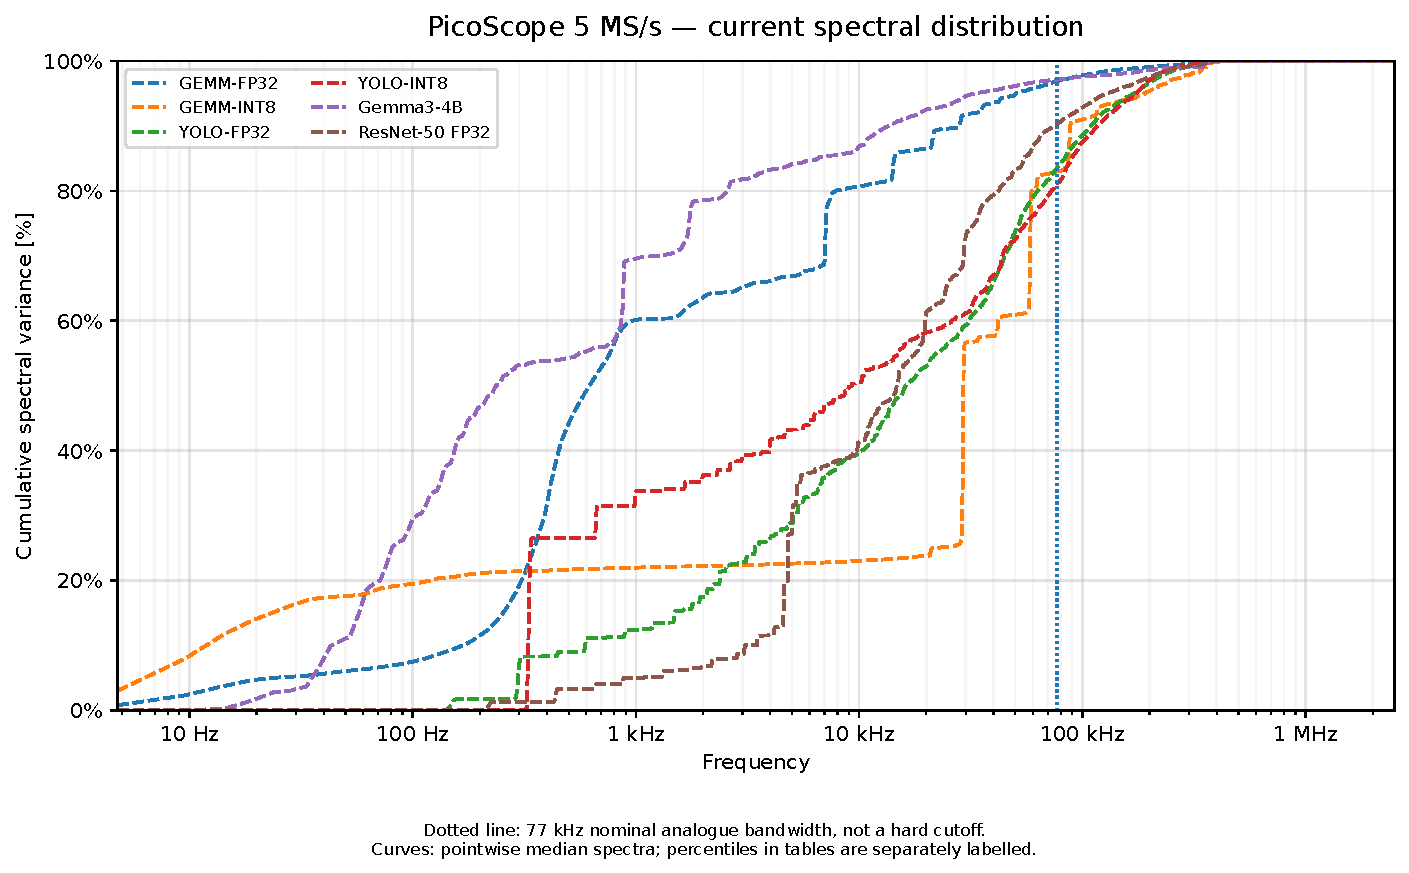
\includegraphics[width=\linewidth]{pico_vs_tek_psd/figures/pico_cross_workload_current_cumulative.pdf}
\caption{Dotted line: 77 kHz nominal analogue bandwidth, not a hard cutoff.
Curves: pointwise median spectra; percentiles in tables are separately labelled.}
\label{fig:journal-pico-vs-tek-psd-figures-pico-cross-workload-current-cumulative}
\end{figure}

\begin{figure}[tbp]
\centering
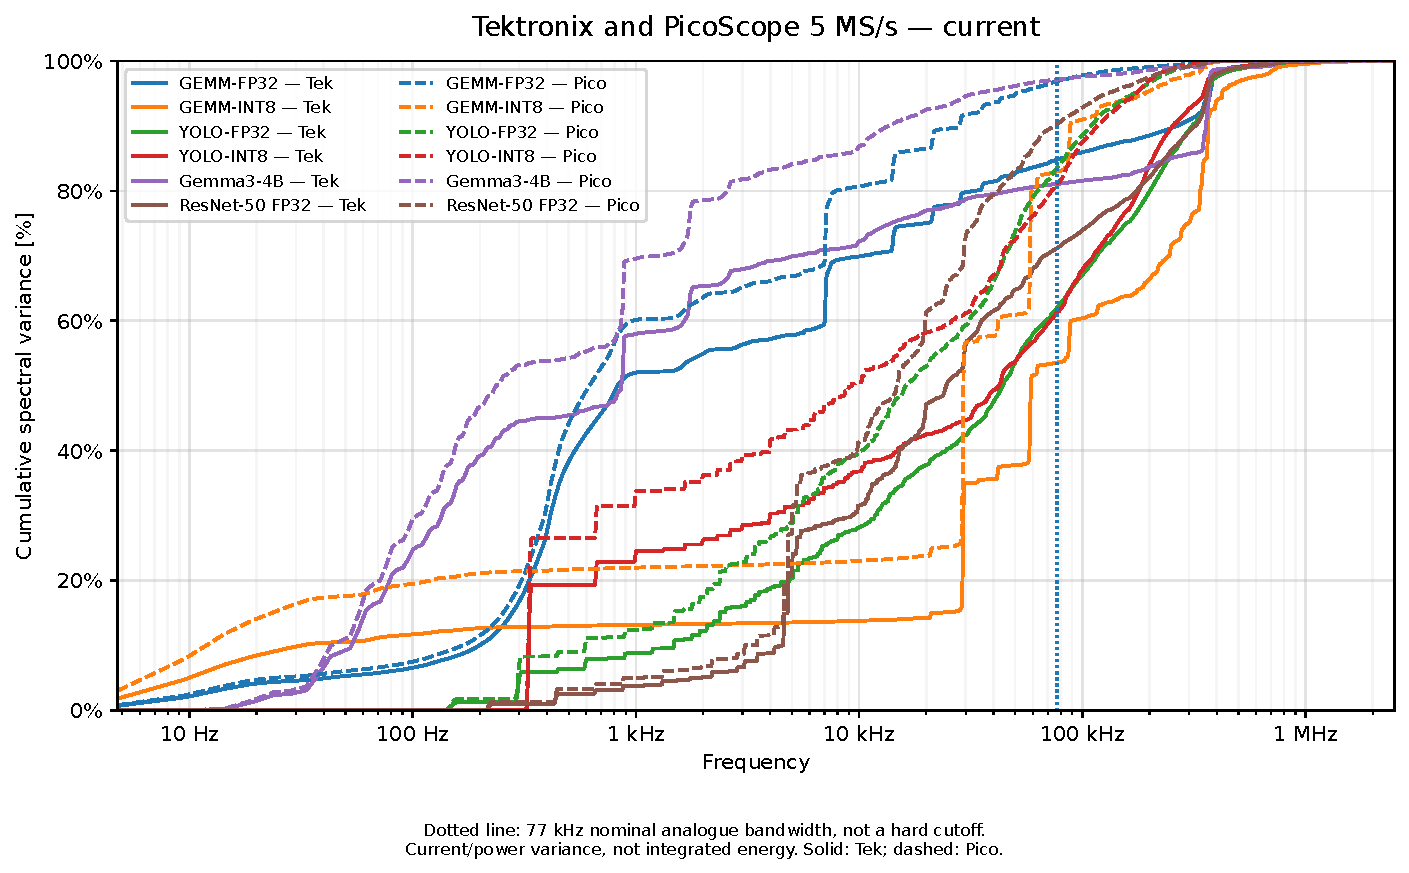
\includegraphics[width=\linewidth]{pico_vs_tek_psd/figures/tek_vs_pico_current_cumulative_overlay.pdf}
\caption{Dotted line: 77 kHz nominal analogue bandwidth, not a hard cutoff.
Current/power variance, not integrated energy. Solid: Tek; dashed: Pico.}
\label{fig:journal-pico-vs-tek-psd-figures-tek-vs-pico-current-cumulative-overlay}
\end{figure}

\begin{figure}[tbp]
\centering
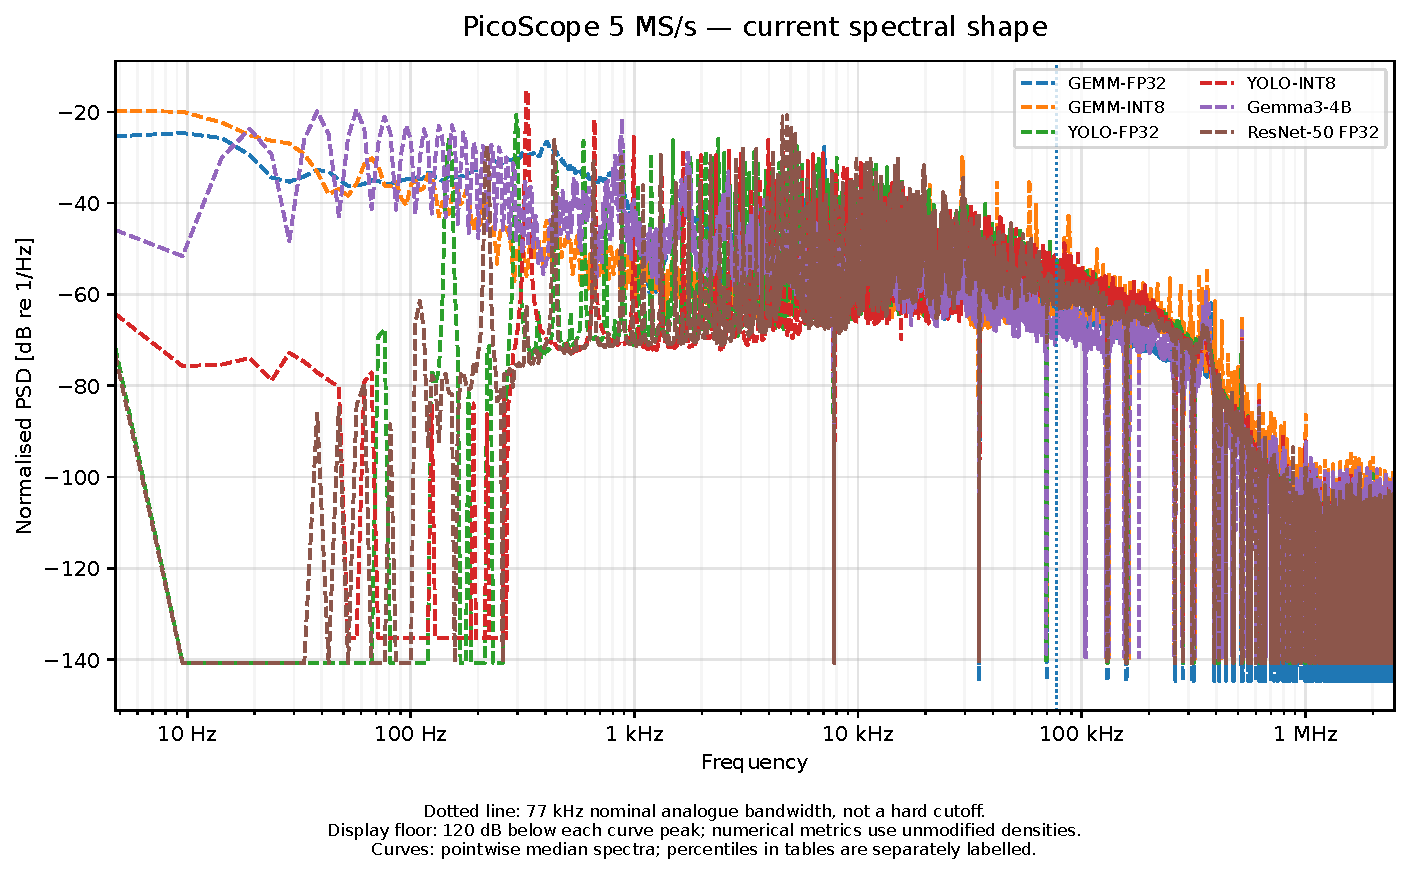
\includegraphics[width=\linewidth]{pico_vs_tek_psd/figures/pico_cross_workload_current_normalised_psd.pdf}
\caption{Dotted line: 77 kHz nominal analogue bandwidth, not a hard cutoff.
Display floor: 120 dB below each curve peak; numerical metrics use unmodified densities.
Curves: pointwise median spectra; percentiles in tables are separately labelled.}
\label{fig:journal-pico-vs-tek-psd-figures-pico-cross-workload-current-normalised-psd}
\end{figure}

\begin{figure}[tbp]
\centering
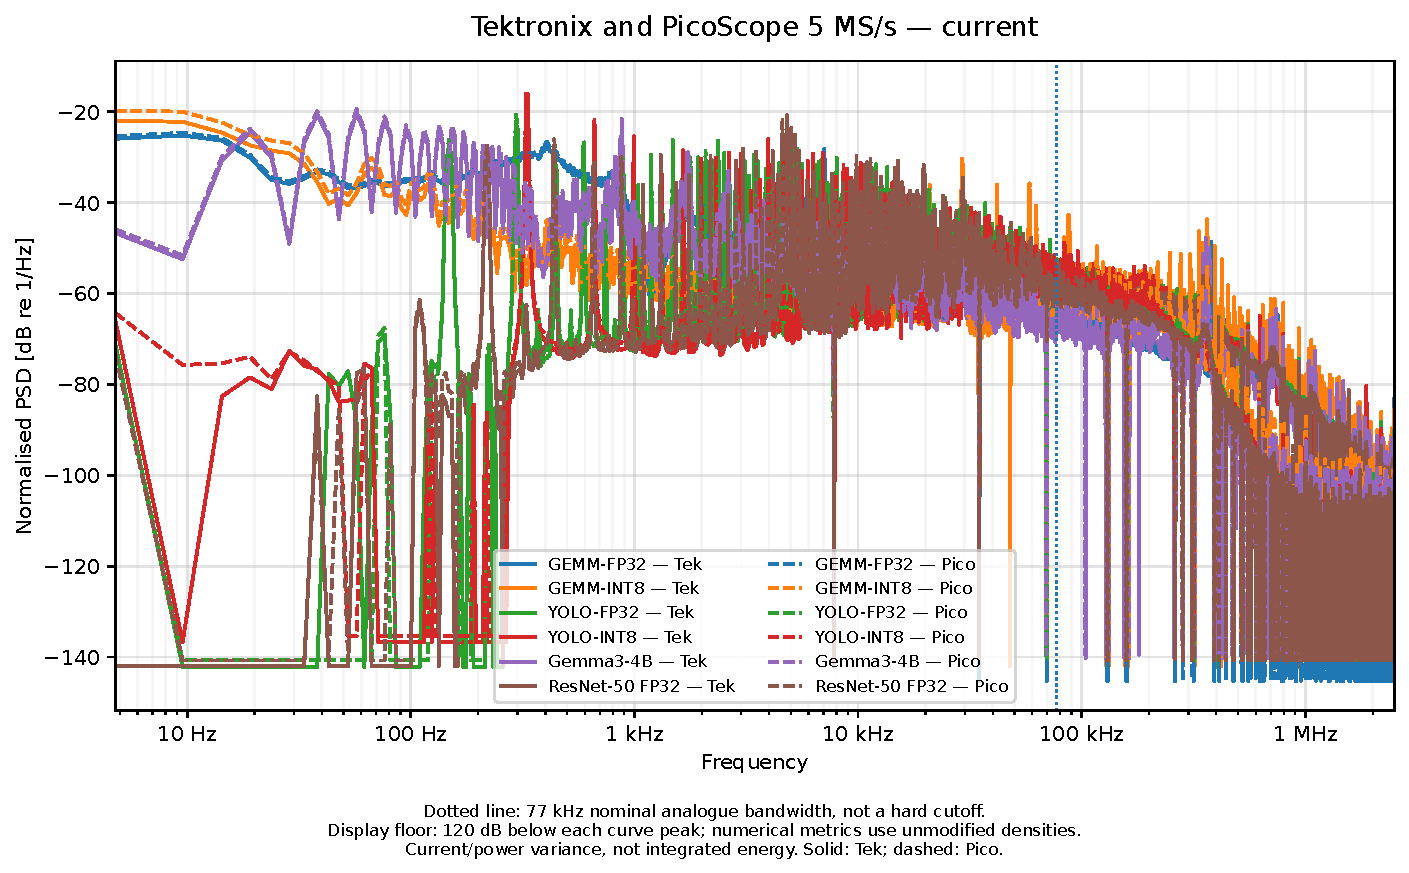
\includegraphics[width=\linewidth]{pico_vs_tek_psd/figures/tek_vs_pico_current_normalised_psd_overlay.pdf}
\caption{Dotted line: 77 kHz nominal analogue bandwidth, not a hard cutoff.
Display floor: 120 dB below each curve peak; numerical metrics use unmodified densities.
Current/power variance, not integrated energy. Solid: Tek; dashed: Pico.}
\label{fig:journal-pico-vs-tek-psd-figures-tek-vs-pico-current-normalised-psd-overlay}
\end{figure}

\begin{figure}[tbp]
\centering
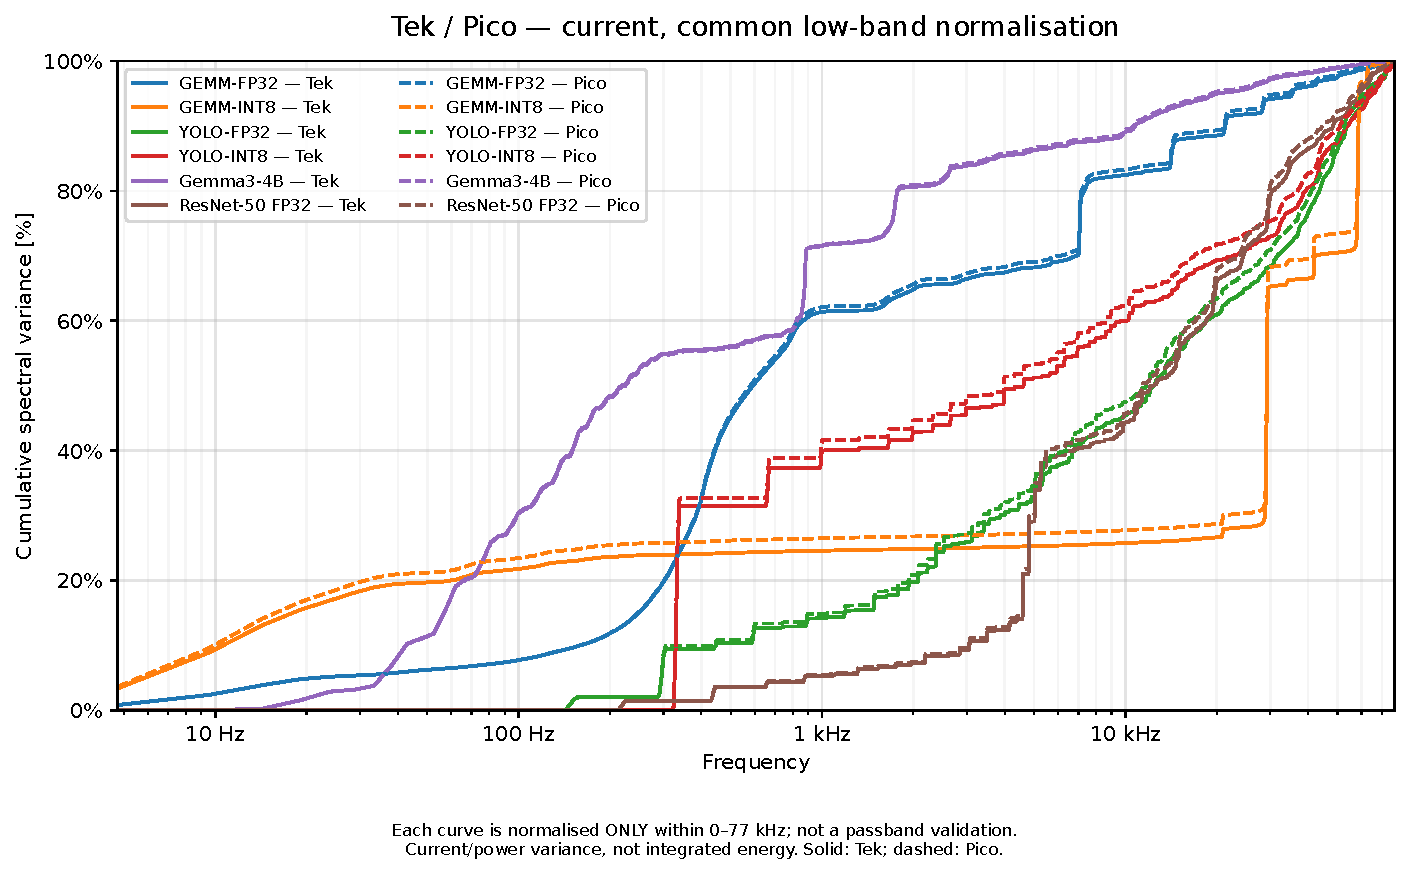
\includegraphics[width=\linewidth]{pico_vs_tek_psd/figures/tek_vs_pico_current_conditional_cumulative_0_77khz.pdf}
\caption{Each curve is normalised ONLY within 0--77 kHz; not a passband validation.
Current/power variance, not integrated energy. Solid: Tek; dashed: Pico.}
\label{fig:journal-pico-vs-tek-psd-figures-tek-vs-pico-current-conditional-cumulative-0-77khz}
\end{figure}

\begin{figure}[tbp]
\centering
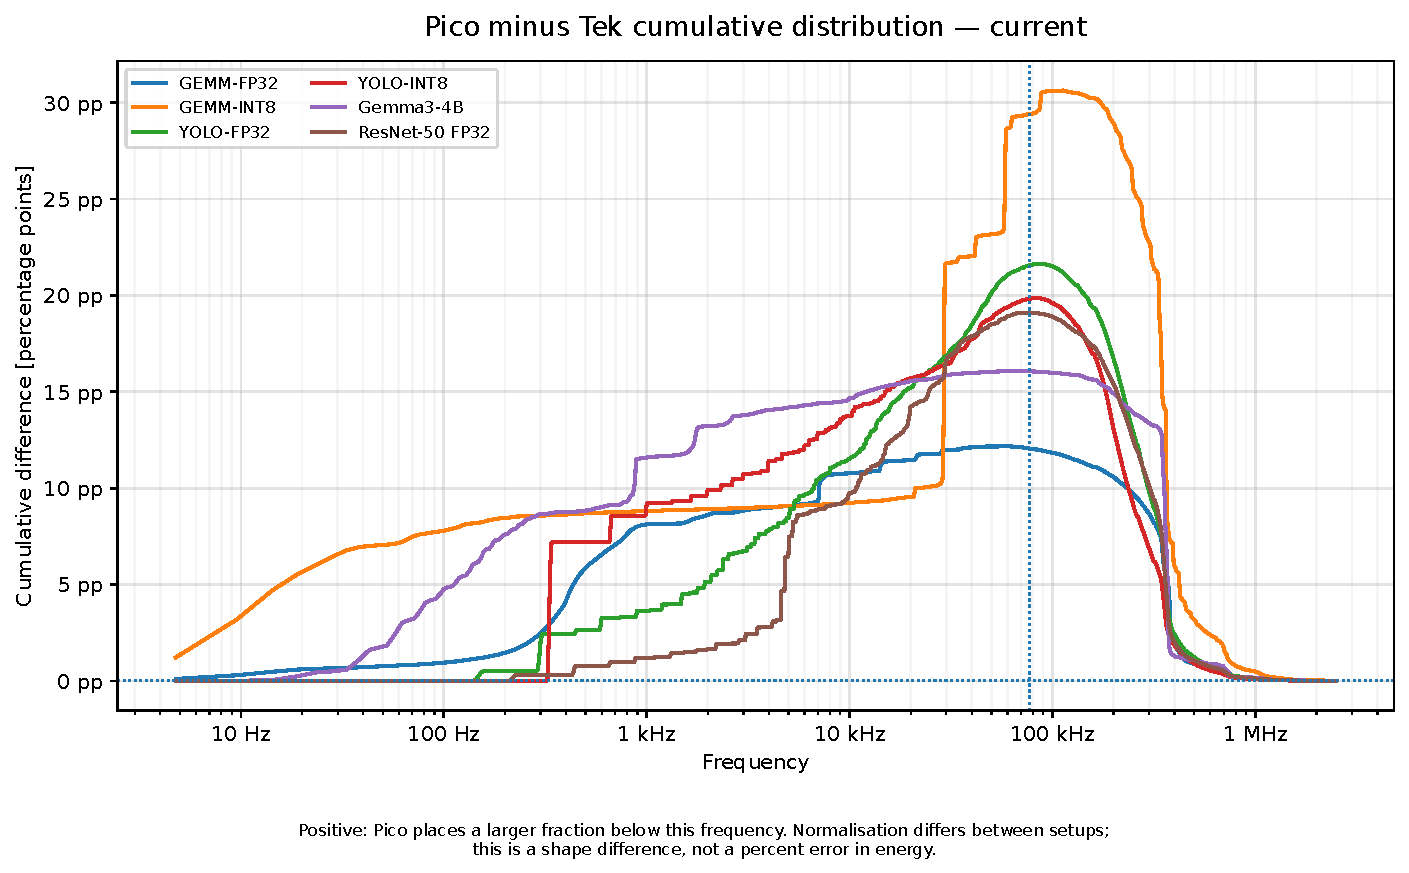
\includegraphics[width=\linewidth]{pico_vs_tek_psd/figures/tek_vs_pico_current_cumulative_difference.pdf}
\caption{Positive: Pico places a larger fraction below this frequency. Normalisation differs between setups;
this is a shape difference, not a percent error in energy.}
\label{fig:journal-pico-vs-tek-psd-figures-tek-vs-pico-current-cumulative-difference}
\end{figure}

\begin{figure}[tbp]
\centering
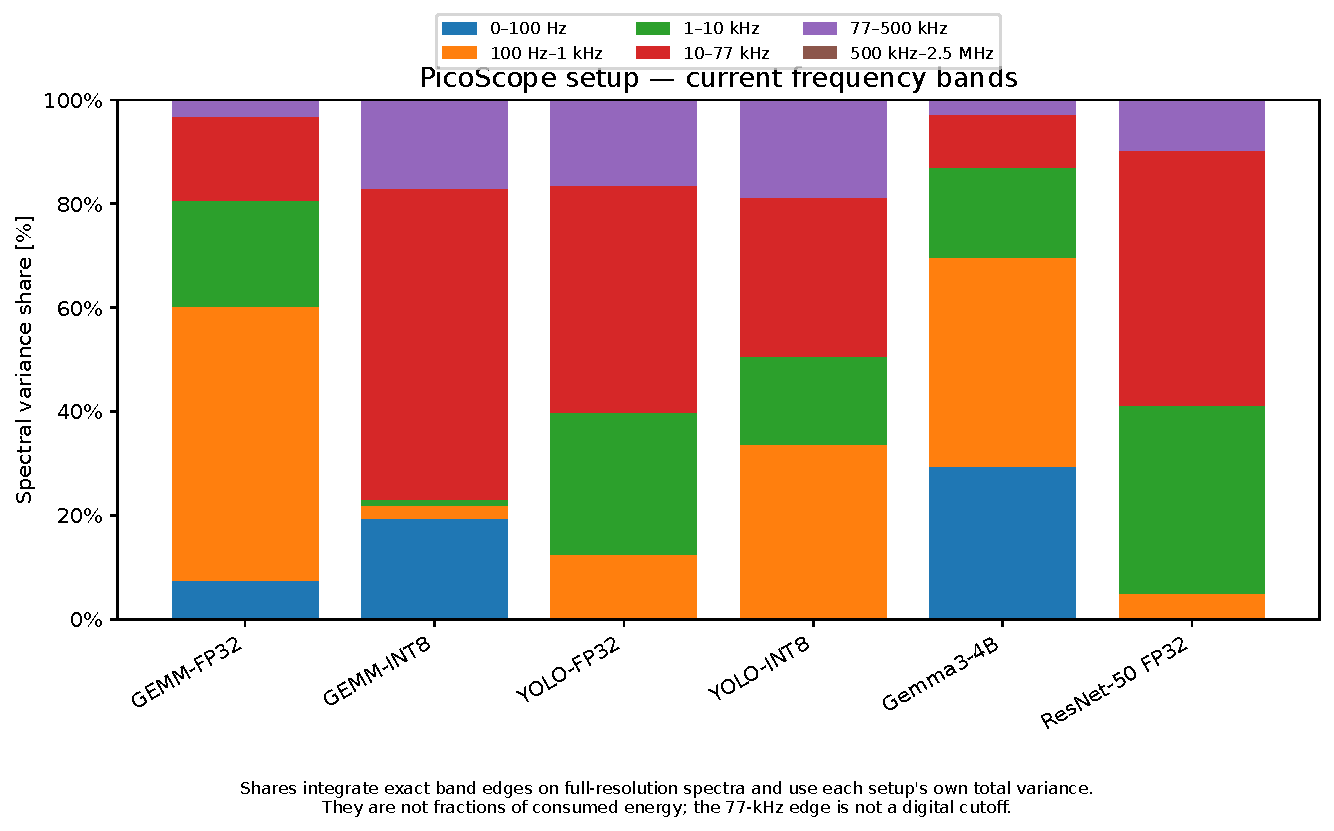
\includegraphics[width=\linewidth]{pico_vs_tek_psd/figures/pico_current_frequency_bands.pdf}
\caption{Shares integrate exact band edges on full-resolution spectra and use each setup's own total variance.
They are not fractions of consumed energy; the 77-kHz edge is not a digital cutoff.}
\label{fig:journal-pico-vs-tek-psd-figures-pico-current-frequency-bands}
\end{figure}

\begin{figure}[tbp]
\centering
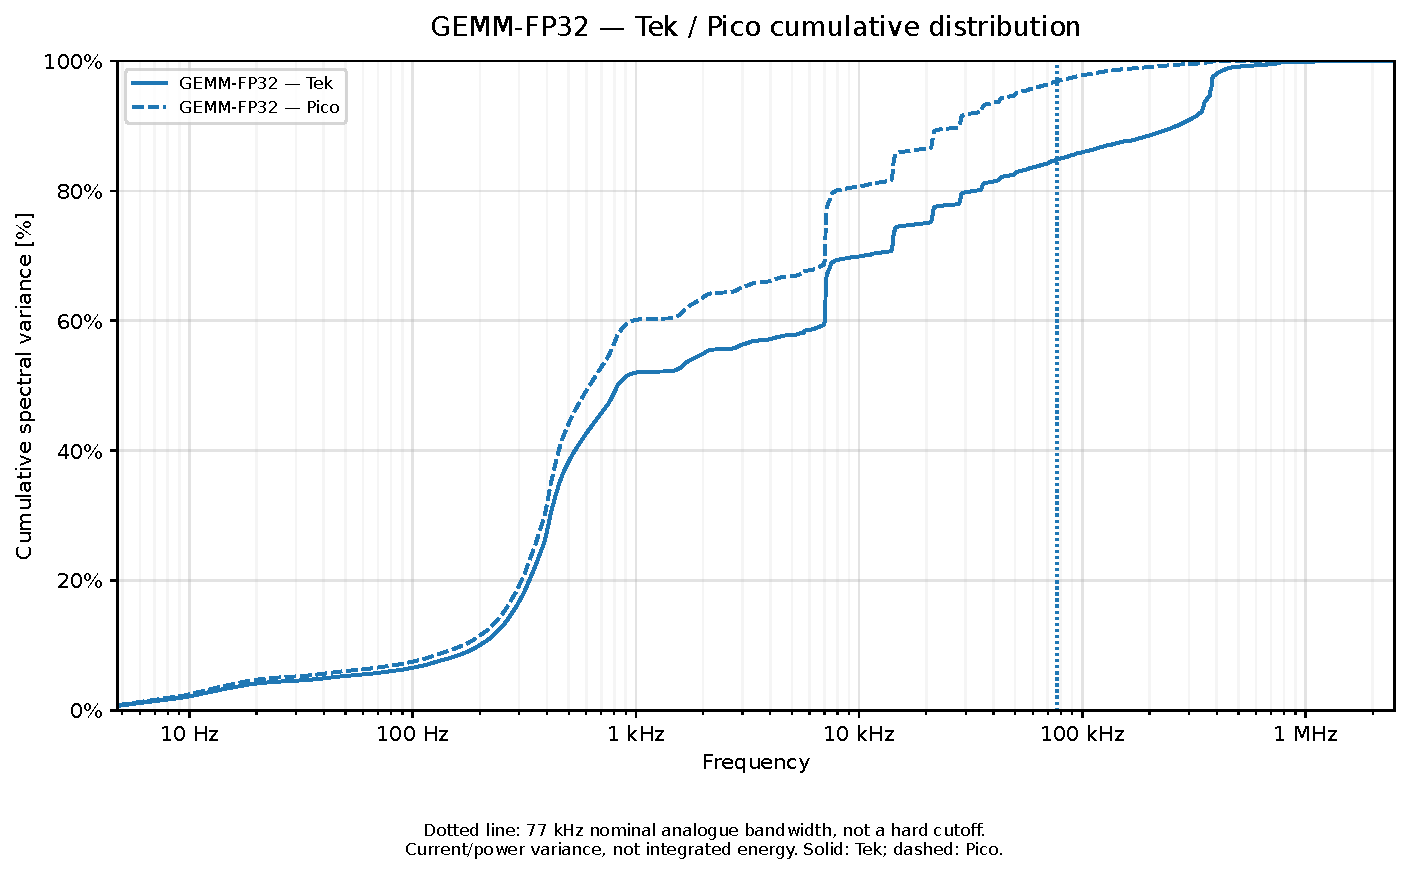
\includegraphics[width=\linewidth]{pico_vs_tek_psd/figures/per_workload/gemmfp32/current_cumulative.pdf}
\caption{Dotted line: 77 kHz nominal analogue bandwidth, not a hard cutoff.
Current/power variance, not integrated energy. Solid: Tek; dashed: Pico.}
\label{fig:journal-pico-vs-tek-psd-figures-per-workload-gemmfp32-current-cumulative}
\end{figure}

\begin{figure}[tbp]
\centering
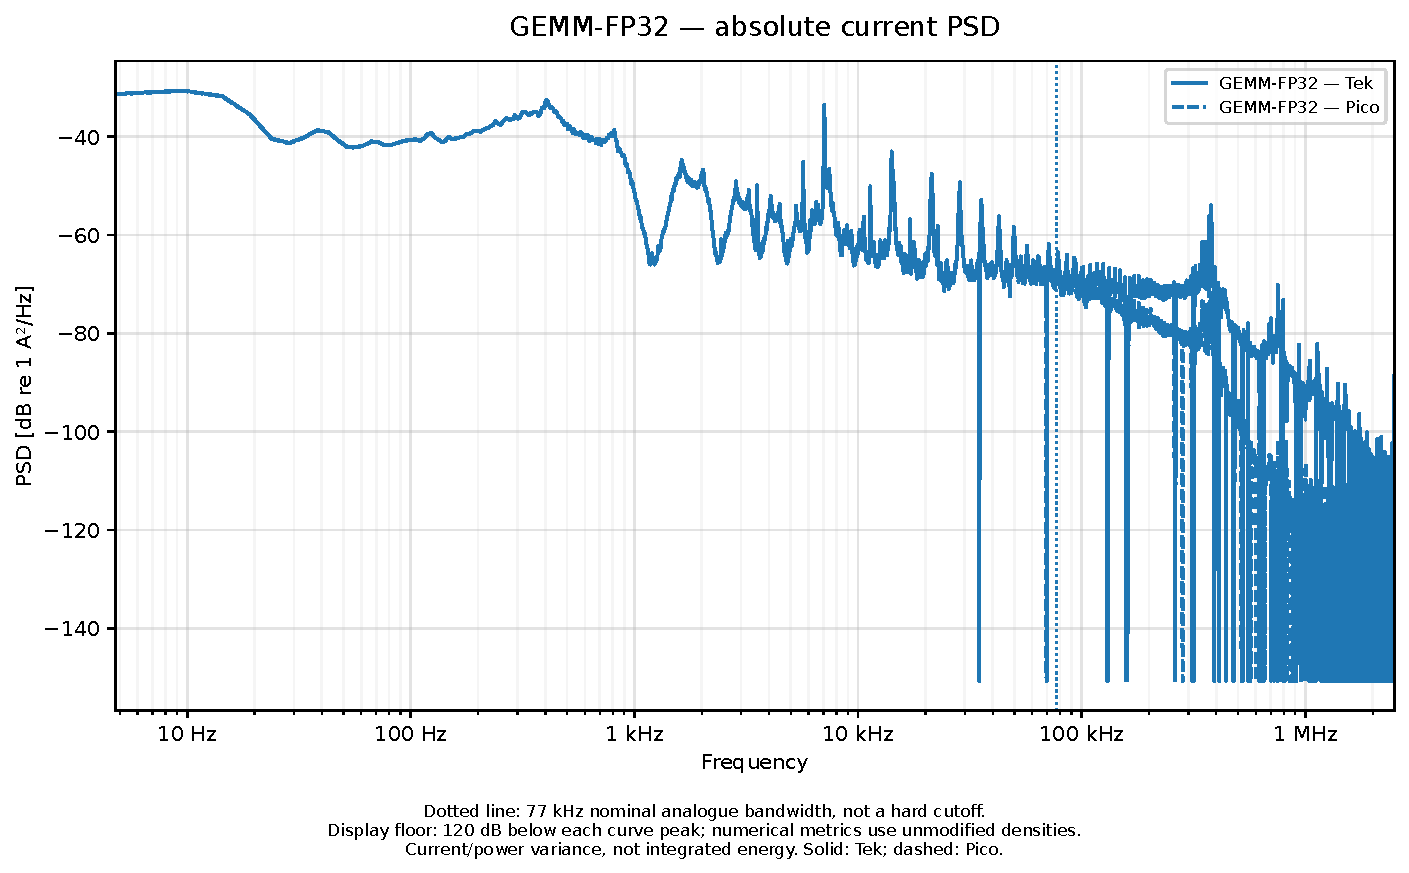
\includegraphics[width=\linewidth]{pico_vs_tek_psd/figures/per_workload/gemmfp32/current_absolute_psd.pdf}
\caption{Dotted line: 77 kHz nominal analogue bandwidth, not a hard cutoff.
Display floor: 120 dB below each curve peak; numerical metrics use unmodified densities.
Current/power variance, not integrated energy. Solid: Tek; dashed: Pico.}
\label{fig:journal-pico-vs-tek-psd-figures-per-workload-gemmfp32-current-absolute-psd}
\end{figure}

\begin{figure}[tbp]
\centering
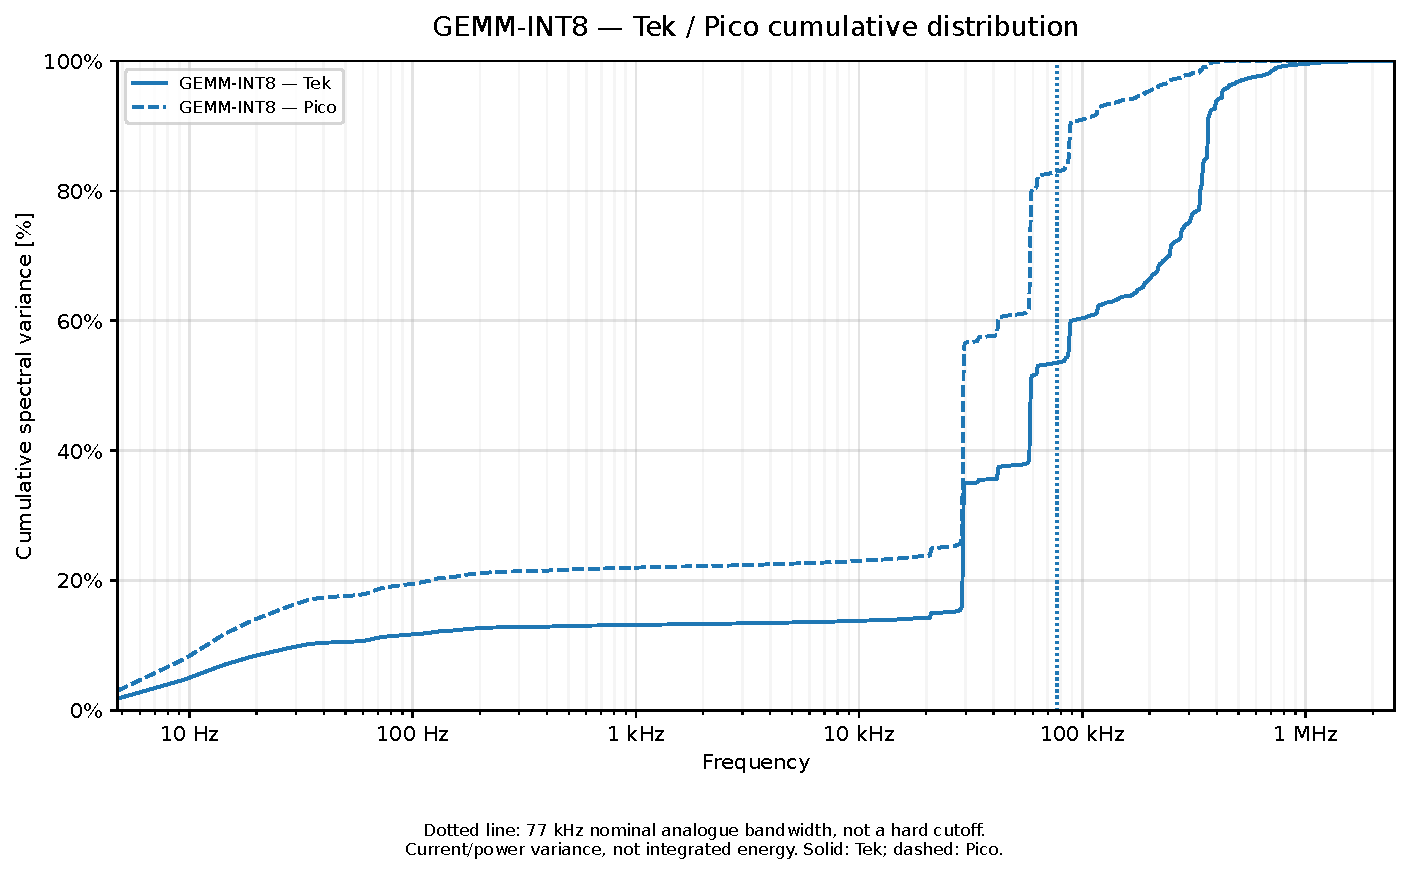
\includegraphics[width=\linewidth]{pico_vs_tek_psd/figures/per_workload/gemmint8/current_cumulative.pdf}
\caption{Dotted line: 77 kHz nominal analogue bandwidth, not a hard cutoff.
Current/power variance, not integrated energy. Solid: Tek; dashed: Pico.}
\label{fig:journal-pico-vs-tek-psd-figures-per-workload-gemmint8-current-cumulative}
\end{figure}

\begin{figure}[tbp]
\centering
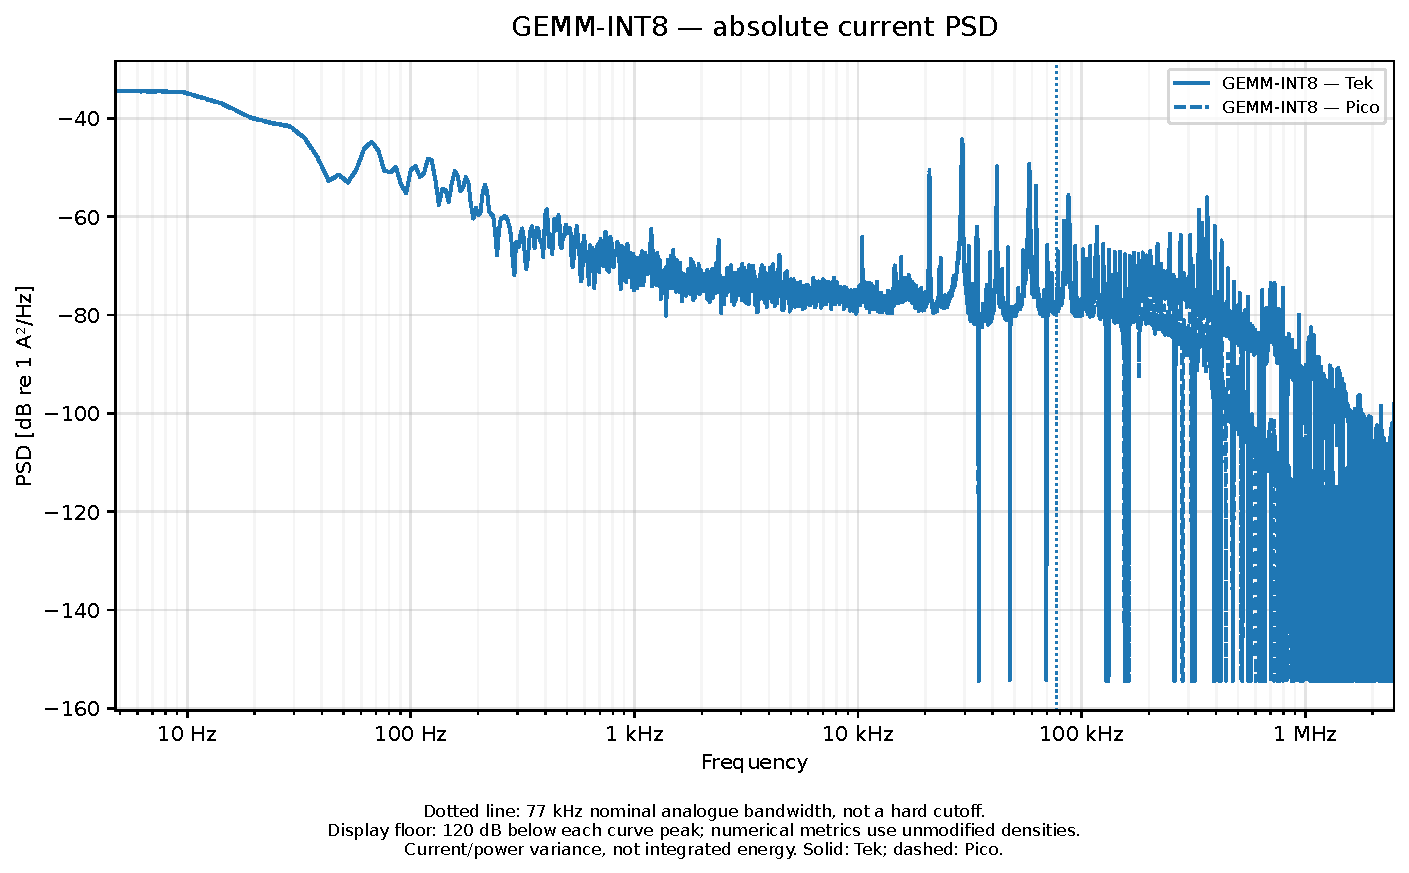
\includegraphics[width=\linewidth]{pico_vs_tek_psd/figures/per_workload/gemmint8/current_absolute_psd.pdf}
\caption{Dotted line: 77 kHz nominal analogue bandwidth, not a hard cutoff.
Display floor: 120 dB below each curve peak; numerical metrics use unmodified densities.
Current/power variance, not integrated energy. Solid: Tek; dashed: Pico.}
\label{fig:journal-pico-vs-tek-psd-figures-per-workload-gemmint8-current-absolute-psd}
\end{figure}

\begin{figure}[tbp]
\centering
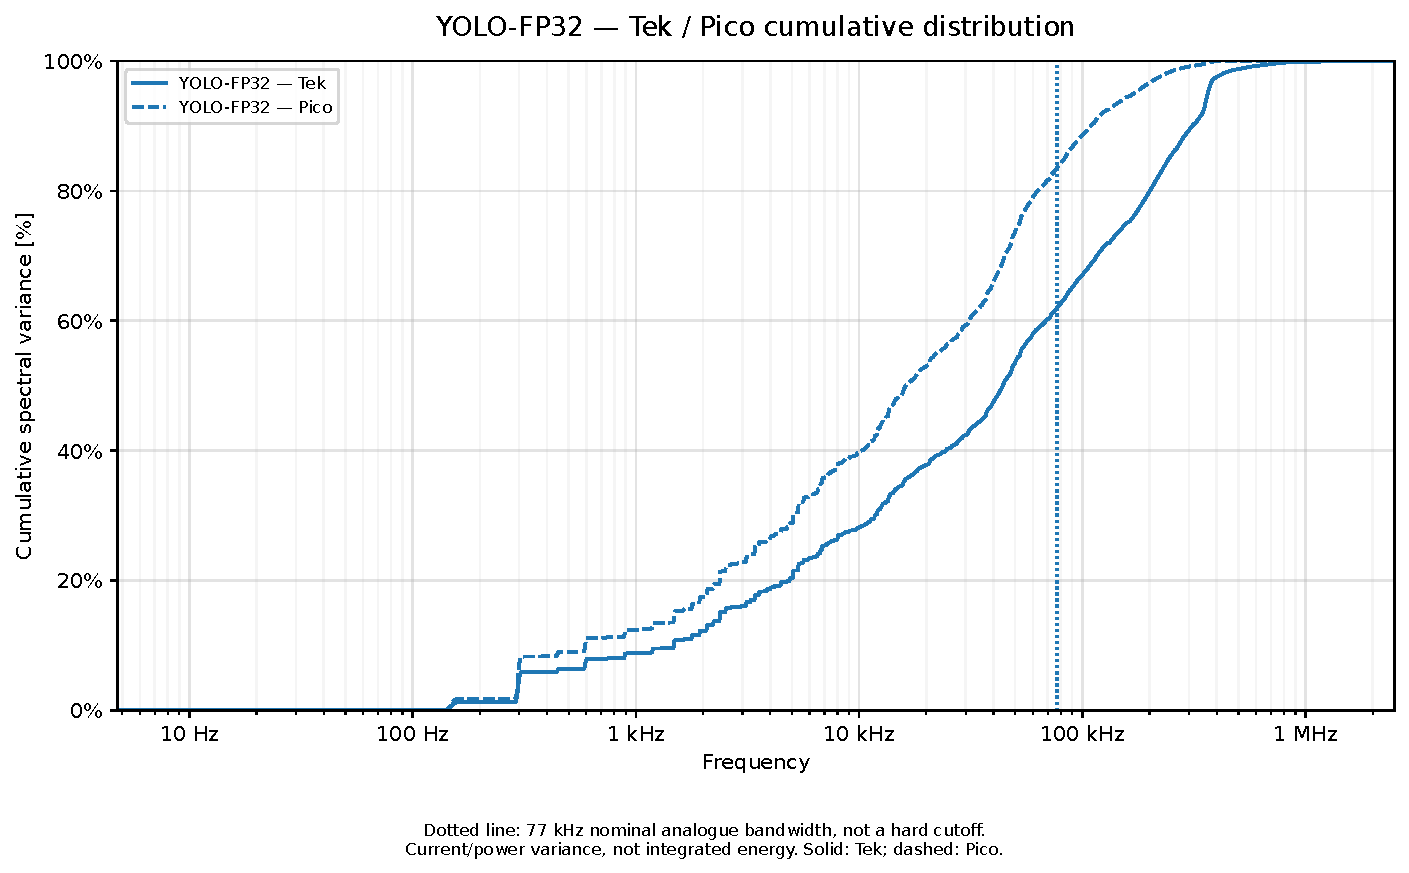
\includegraphics[width=\linewidth]{pico_vs_tek_psd/figures/per_workload/yolofp32/current_cumulative.pdf}
\caption{Dotted line: 77 kHz nominal analogue bandwidth, not a hard cutoff.
Current/power variance, not integrated energy. Solid: Tek; dashed: Pico.}
\label{fig:journal-pico-vs-tek-psd-figures-per-workload-yolofp32-current-cumulative}
\end{figure}

\begin{figure}[tbp]
\centering
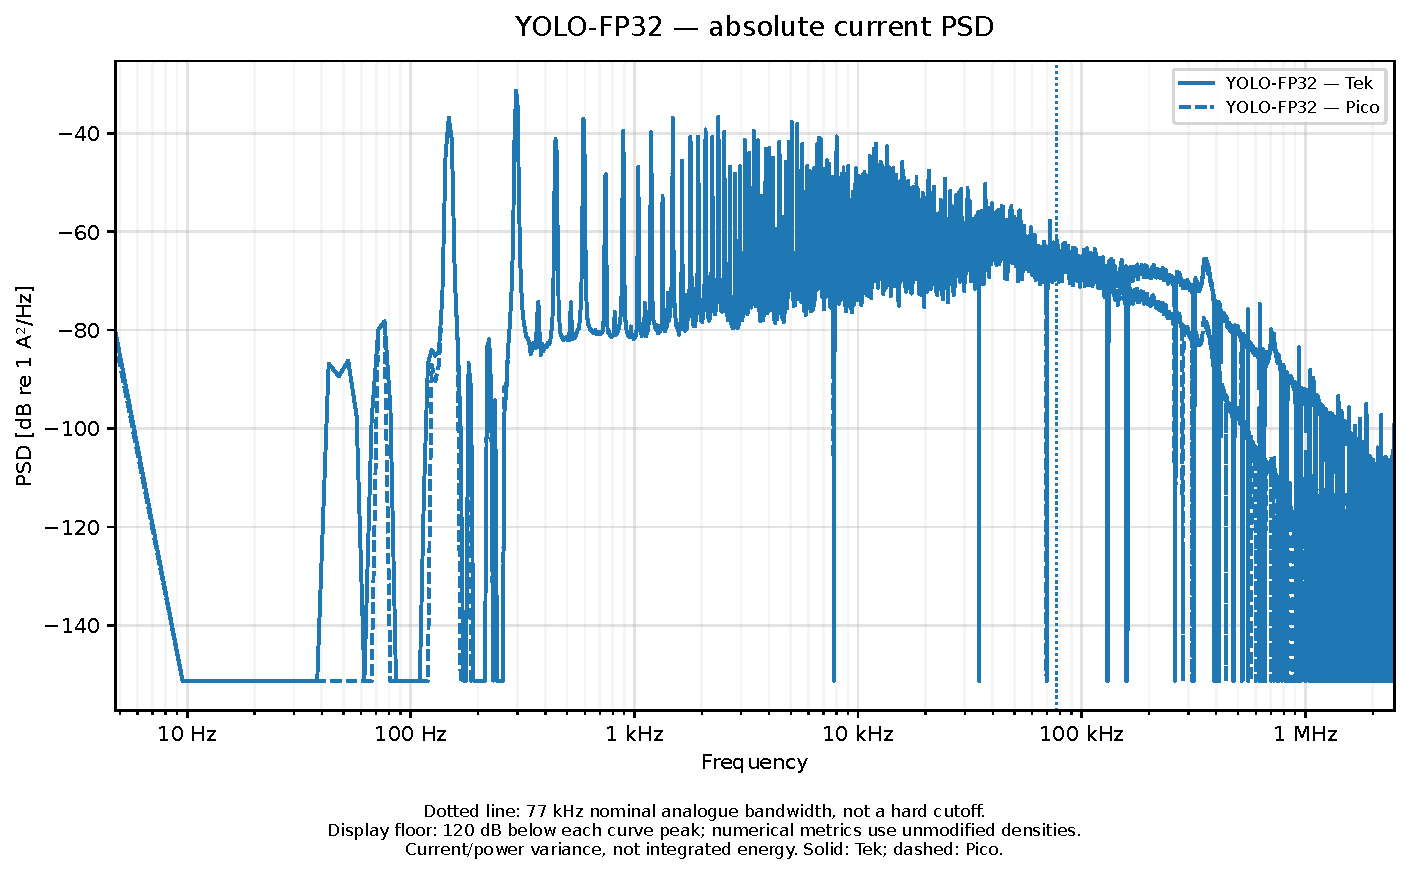
\includegraphics[width=\linewidth]{pico_vs_tek_psd/figures/per_workload/yolofp32/current_absolute_psd.pdf}
\caption{Dotted line: 77 kHz nominal analogue bandwidth, not a hard cutoff.
Display floor: 120 dB below each curve peak; numerical metrics use unmodified densities.
Current/power variance, not integrated energy. Solid: Tek; dashed: Pico.}
\label{fig:journal-pico-vs-tek-psd-figures-per-workload-yolofp32-current-absolute-psd}
\end{figure}

\begin{figure}[tbp]
\centering
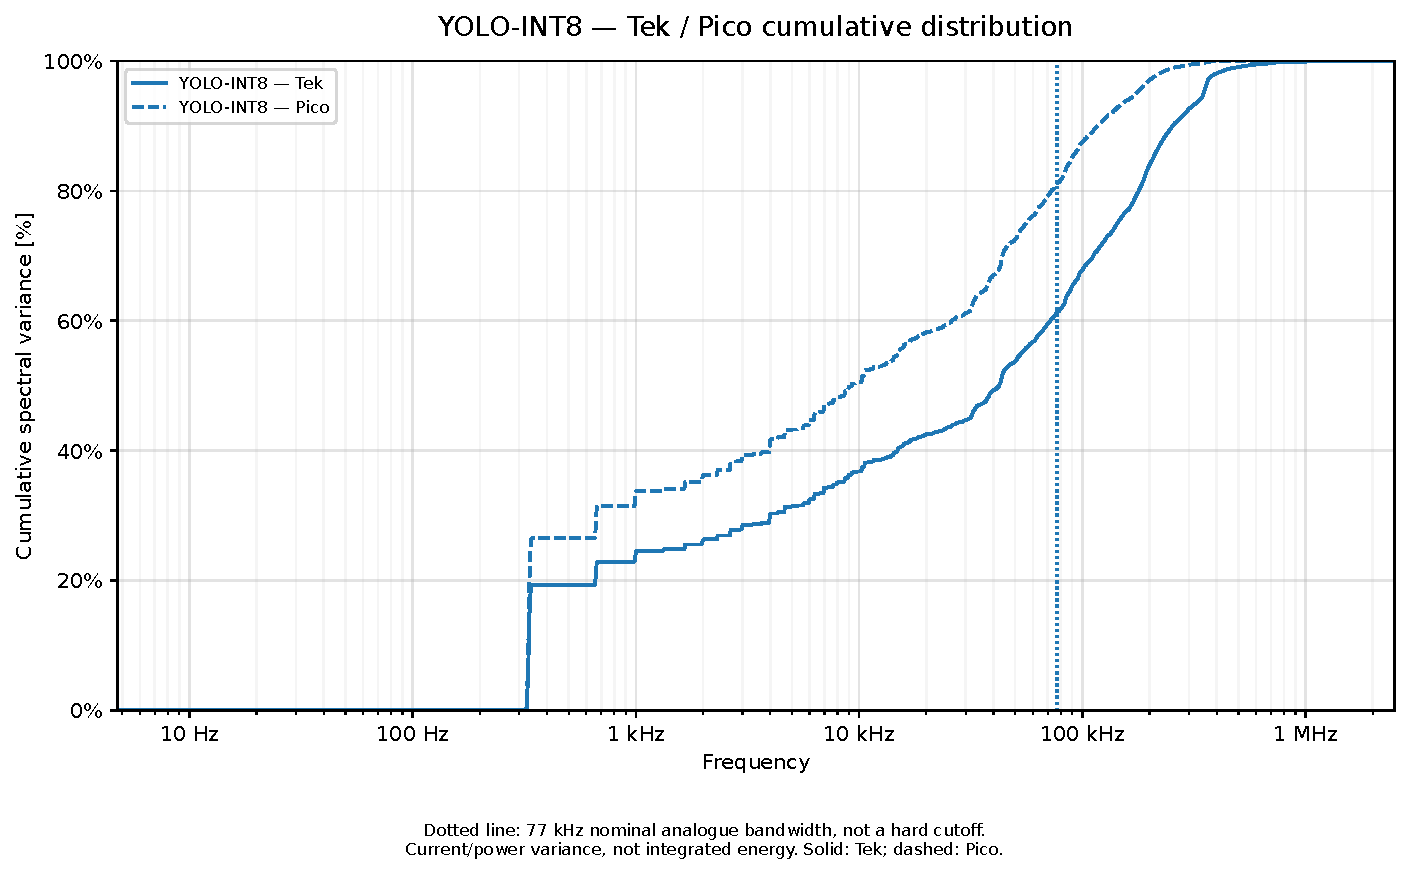
\includegraphics[width=\linewidth]{pico_vs_tek_psd/figures/per_workload/yoloint8/current_cumulative.pdf}
\caption{Dotted line: 77 kHz nominal analogue bandwidth, not a hard cutoff.
Current/power variance, not integrated energy. Solid: Tek; dashed: Pico.}
\label{fig:journal-pico-vs-tek-psd-figures-per-workload-yoloint8-current-cumulative}
\end{figure}

\begin{figure}[tbp]
\centering
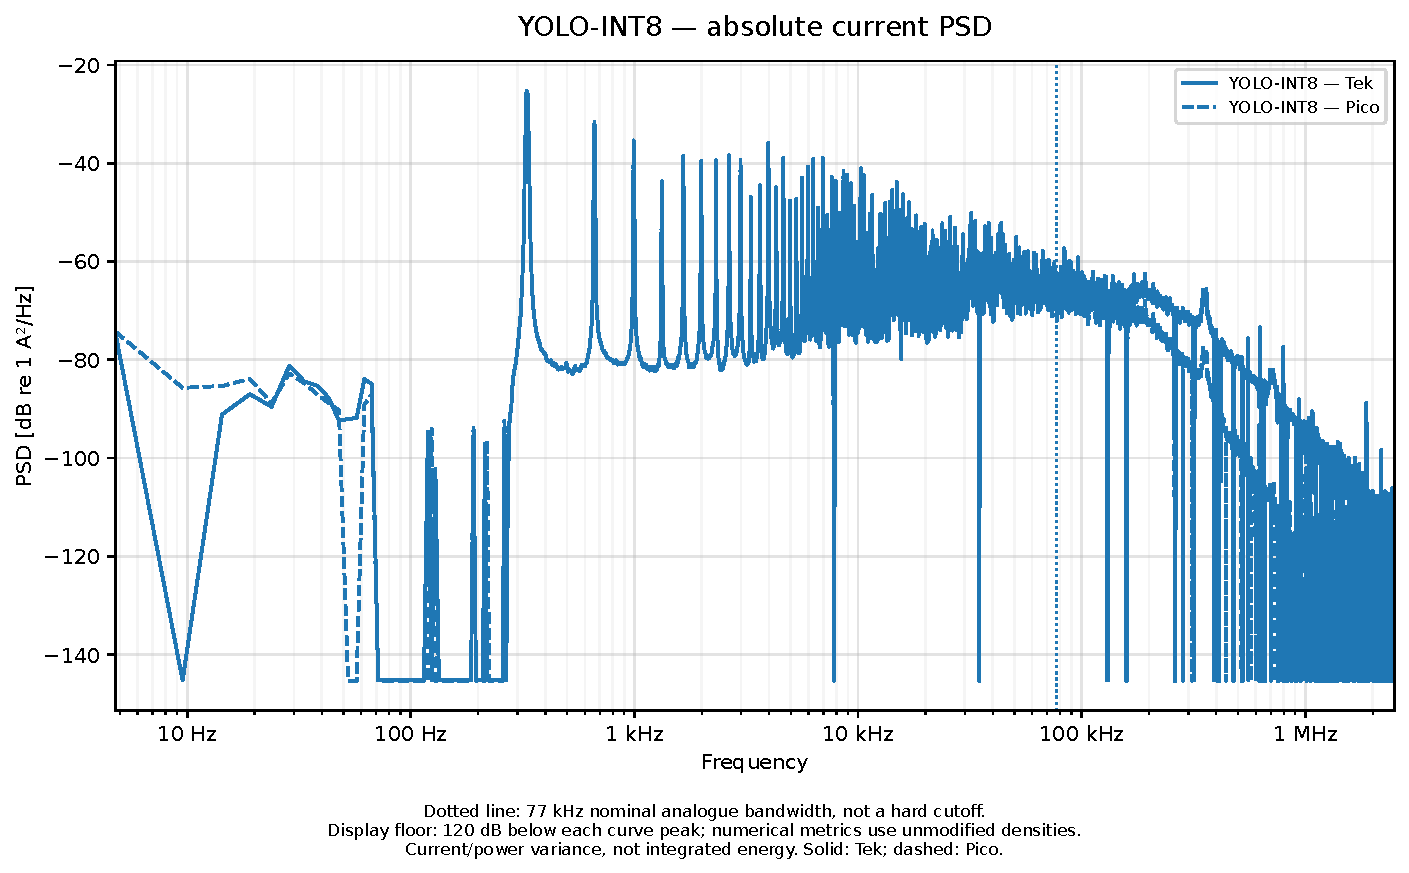
\includegraphics[width=\linewidth]{pico_vs_tek_psd/figures/per_workload/yoloint8/current_absolute_psd.pdf}
\caption{Dotted line: 77 kHz nominal analogue bandwidth, not a hard cutoff.
Display floor: 120 dB below each curve peak; numerical metrics use unmodified densities.
Current/power variance, not integrated energy. Solid: Tek; dashed: Pico.}
\label{fig:journal-pico-vs-tek-psd-figures-per-workload-yoloint8-current-absolute-psd}
\end{figure}

\begin{figure}[tbp]
\centering
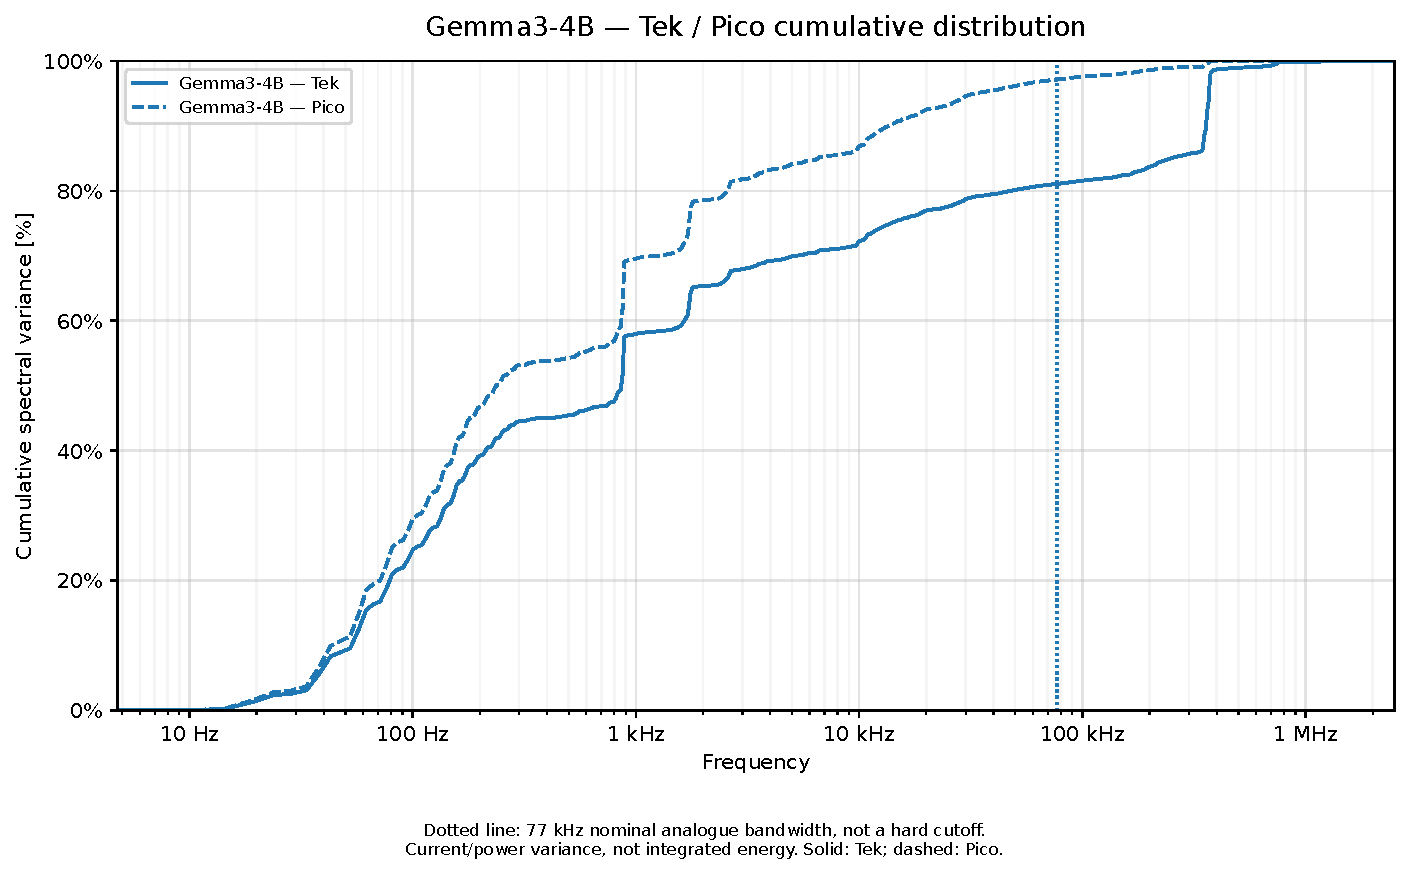
\includegraphics[width=\linewidth]{pico_vs_tek_psd/figures/per_workload/gemma3-4b/current_cumulative.pdf}
\caption{Dotted line: 77 kHz nominal analogue bandwidth, not a hard cutoff.
Current/power variance, not integrated energy. Solid: Tek; dashed: Pico.}
\label{fig:journal-pico-vs-tek-psd-figures-per-workload-gemma3-4b-current-cumulative}
\end{figure}

\begin{figure}[tbp]
\centering
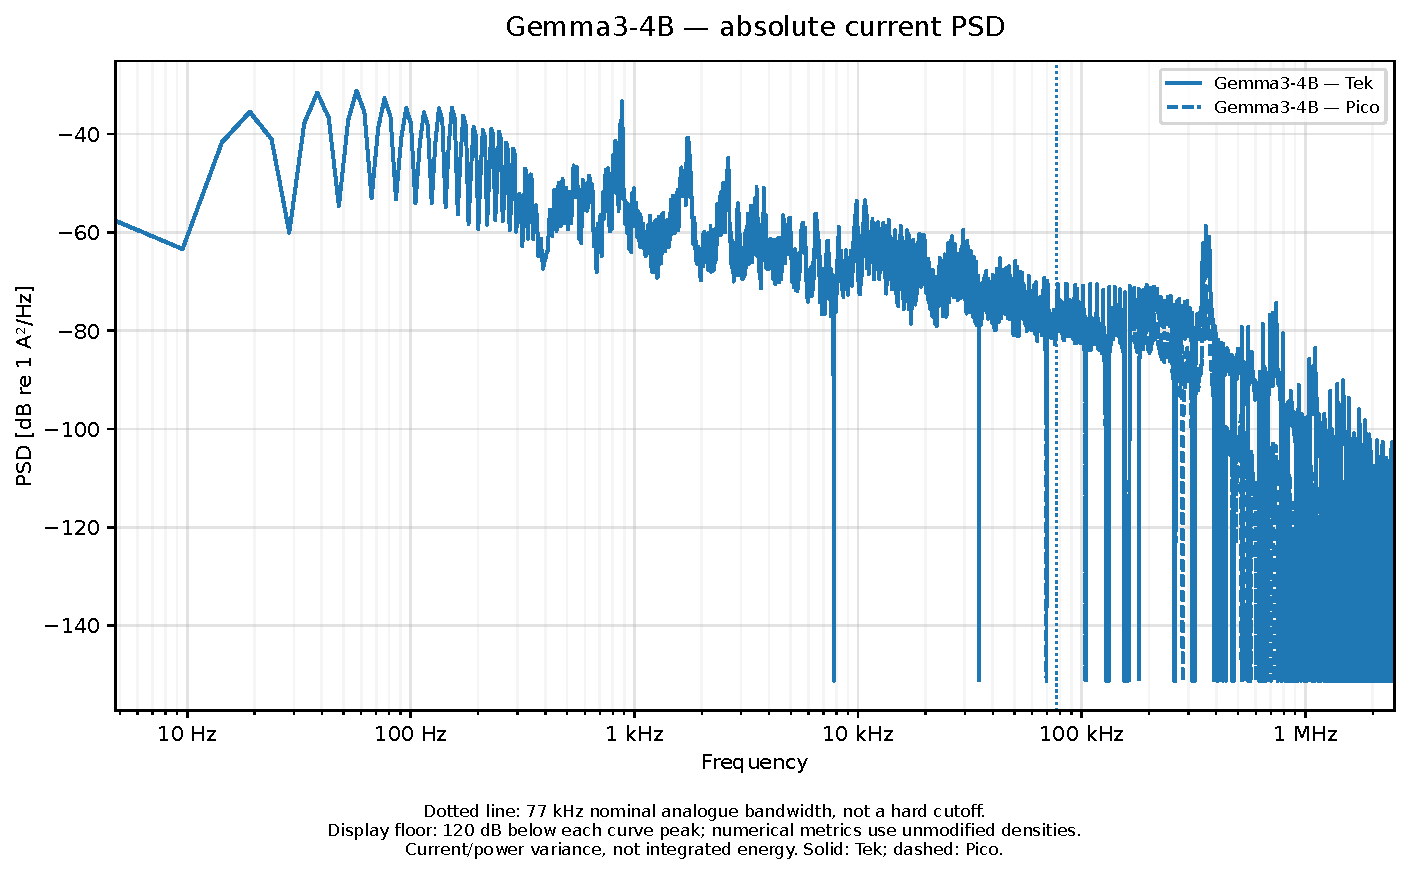
\includegraphics[width=\linewidth]{pico_vs_tek_psd/figures/per_workload/gemma3-4b/current_absolute_psd.pdf}
\caption{Dotted line: 77 kHz nominal analogue bandwidth, not a hard cutoff.
Display floor: 120 dB below each curve peak; numerical metrics use unmodified densities.
Current/power variance, not integrated energy. Solid: Tek; dashed: Pico.}
\label{fig:journal-pico-vs-tek-psd-figures-per-workload-gemma3-4b-current-absolute-psd}
\end{figure}

\begin{figure}[tbp]
\centering
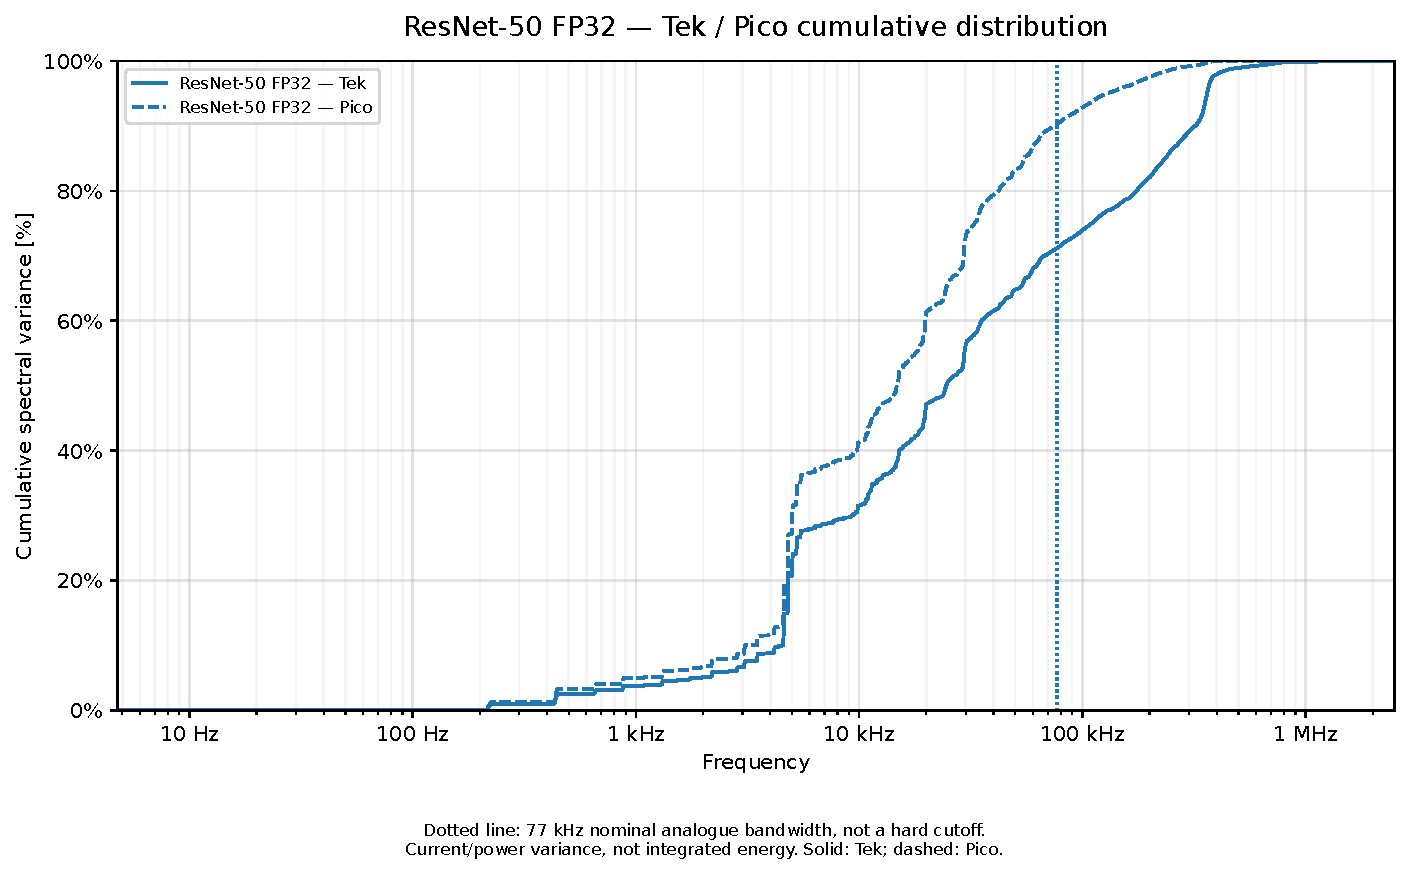
\includegraphics[width=\linewidth]{pico_vs_tek_psd/figures/per_workload/resnet50/current_cumulative.pdf}
\caption{Dotted line: 77 kHz nominal analogue bandwidth, not a hard cutoff.
Current/power variance, not integrated energy. Solid: Tek; dashed: Pico.}
\label{fig:journal-pico-vs-tek-psd-figures-per-workload-resnet50-current-cumulative}
\end{figure}

\begin{figure}[tbp]
\centering
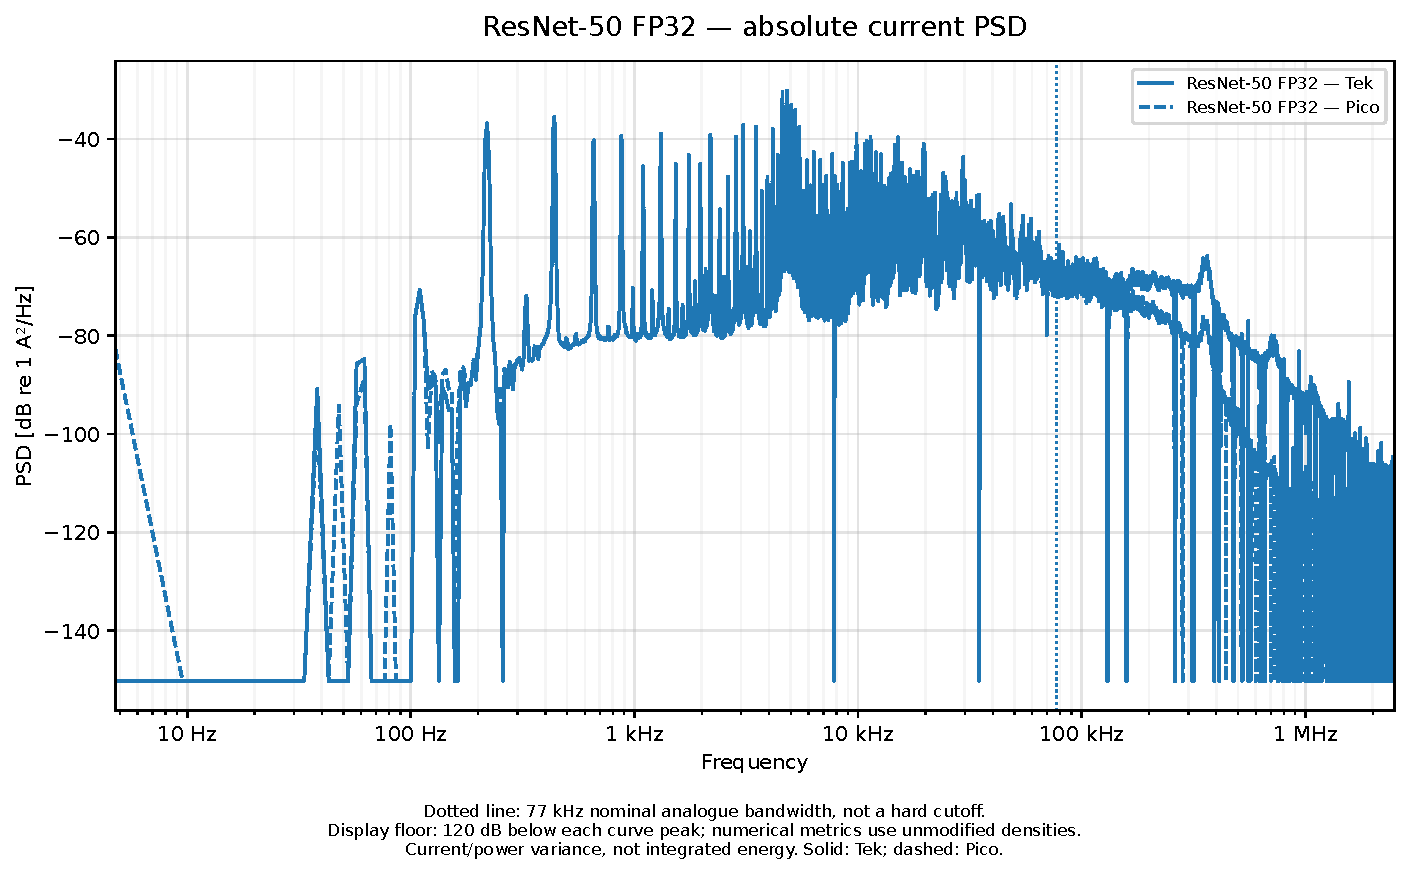
\includegraphics[width=\linewidth]{pico_vs_tek_psd/figures/per_workload/resnet50/current_absolute_psd.pdf}
\caption{Dotted line: 77 kHz nominal analogue bandwidth, not a hard cutoff.
Display floor: 120 dB below each curve peak; numerical metrics use unmodified densities.
Current/power variance, not integrated energy. Solid: Tek; dashed: Pico.}
\label{fig:journal-pico-vs-tek-psd-figures-per-workload-resnet50-current-absolute-psd}
\end{figure}

\begin{figure}[tbp]
\centering
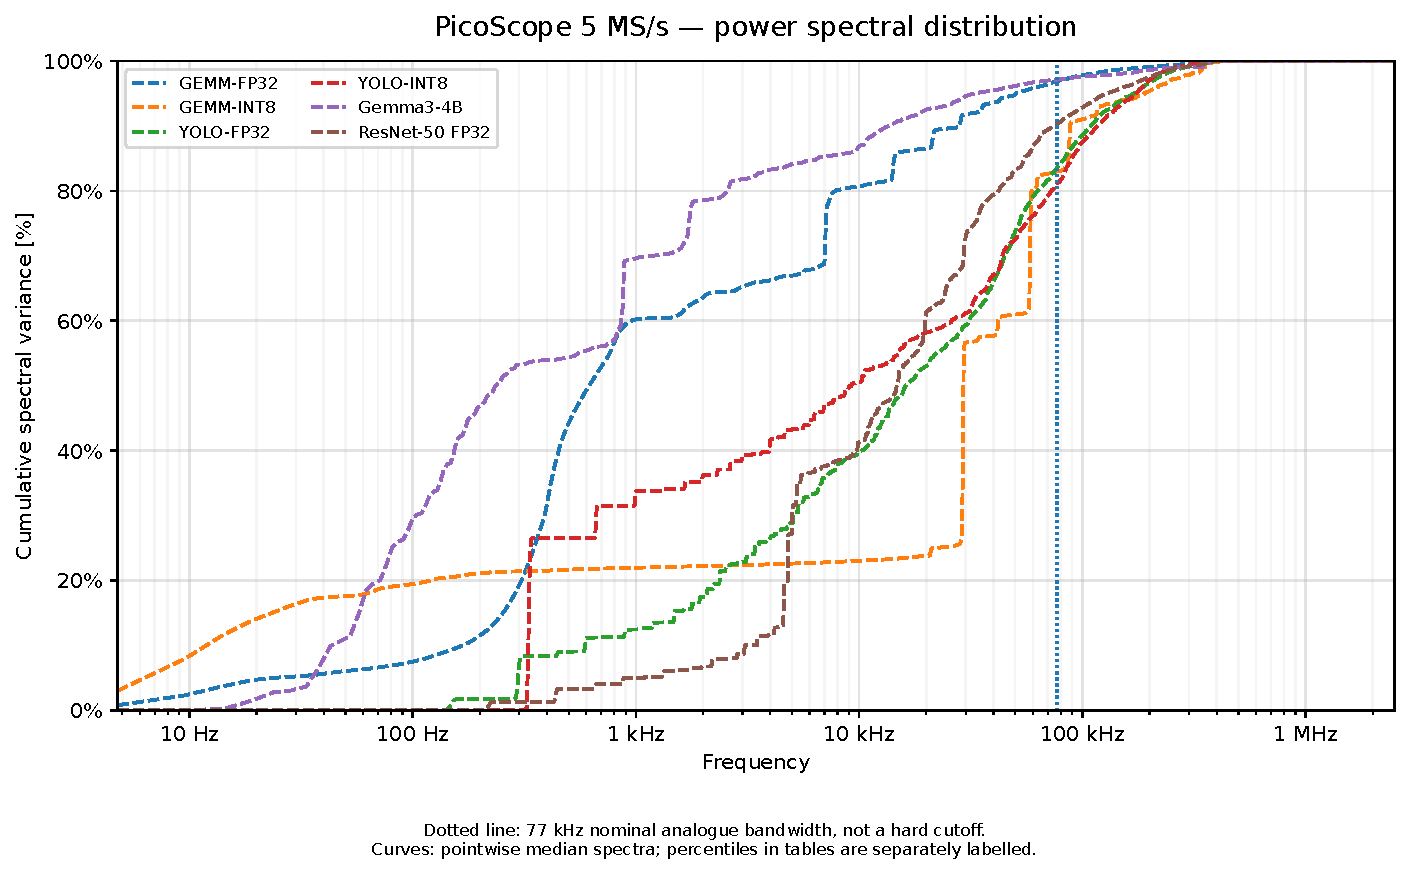
\includegraphics[width=\linewidth]{pico_vs_tek_psd/figures/pico_cross_workload_power_cumulative.pdf}
\caption{Dotted line: 77 kHz nominal analogue bandwidth, not a hard cutoff.
Curves: pointwise median spectra; percentiles in tables are separately labelled.}
\label{fig:journal-pico-vs-tek-psd-figures-pico-cross-workload-power-cumulative}
\end{figure}

\begin{figure}[tbp]
\centering
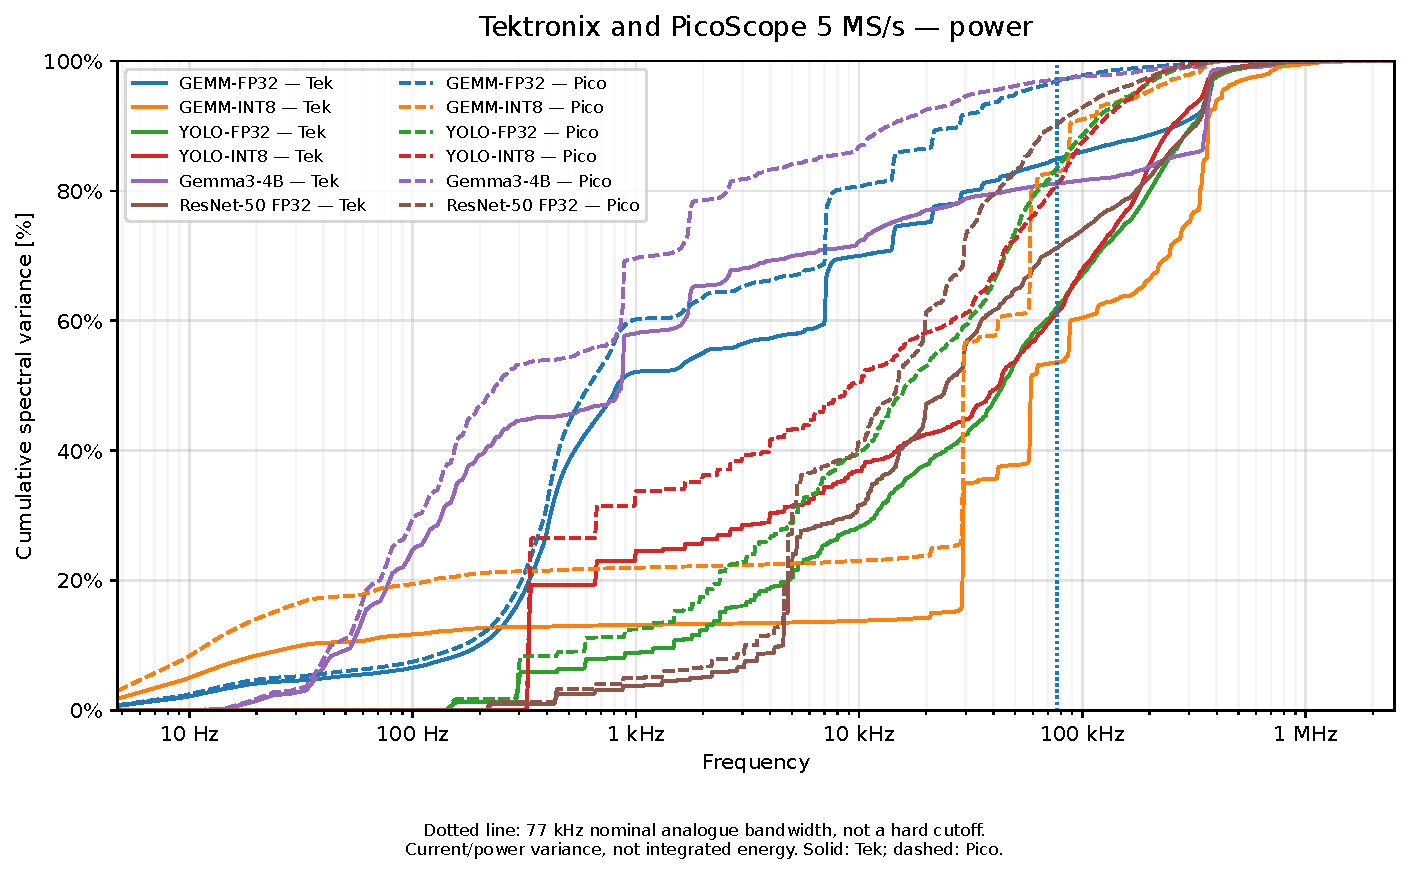
\includegraphics[width=\linewidth]{pico_vs_tek_psd/figures/tek_vs_pico_power_cumulative_overlay.pdf}
\caption{Dotted line: 77 kHz nominal analogue bandwidth, not a hard cutoff.
Current/power variance, not integrated energy. Solid: Tek; dashed: Pico.}
\label{fig:journal-pico-vs-tek-psd-figures-tek-vs-pico-power-cumulative-overlay}
\end{figure}

\begin{figure}[tbp]
\centering
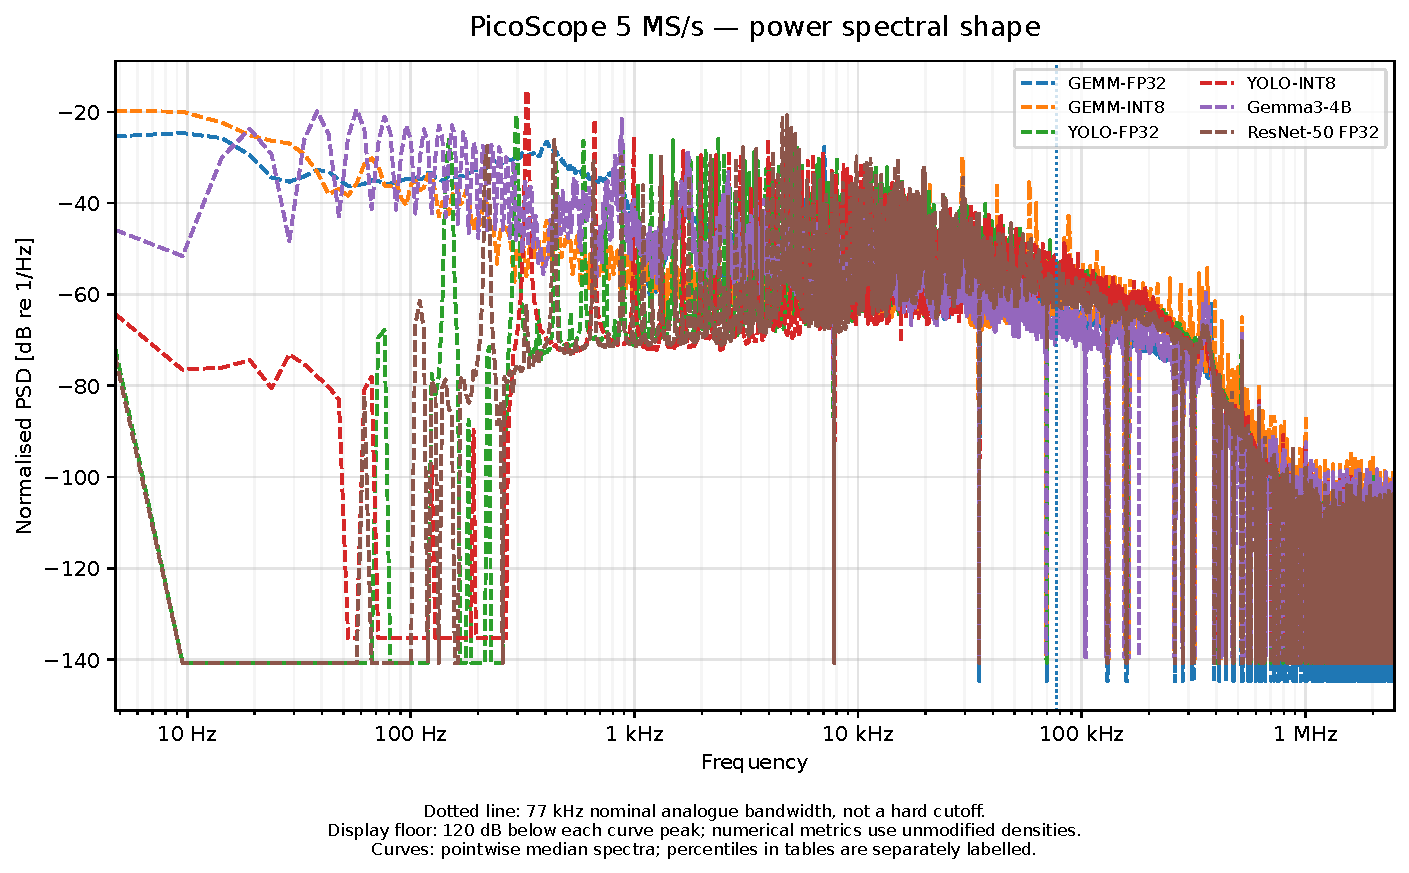
\includegraphics[width=\linewidth]{pico_vs_tek_psd/figures/pico_cross_workload_power_normalised_psd.pdf}
\caption{Dotted line: 77 kHz nominal analogue bandwidth, not a hard cutoff.
Display floor: 120 dB below each curve peak; numerical metrics use unmodified densities.
Curves: pointwise median spectra; percentiles in tables are separately labelled.}
\label{fig:journal-pico-vs-tek-psd-figures-pico-cross-workload-power-normalised-psd}
\end{figure}

\begin{figure}[tbp]
\centering
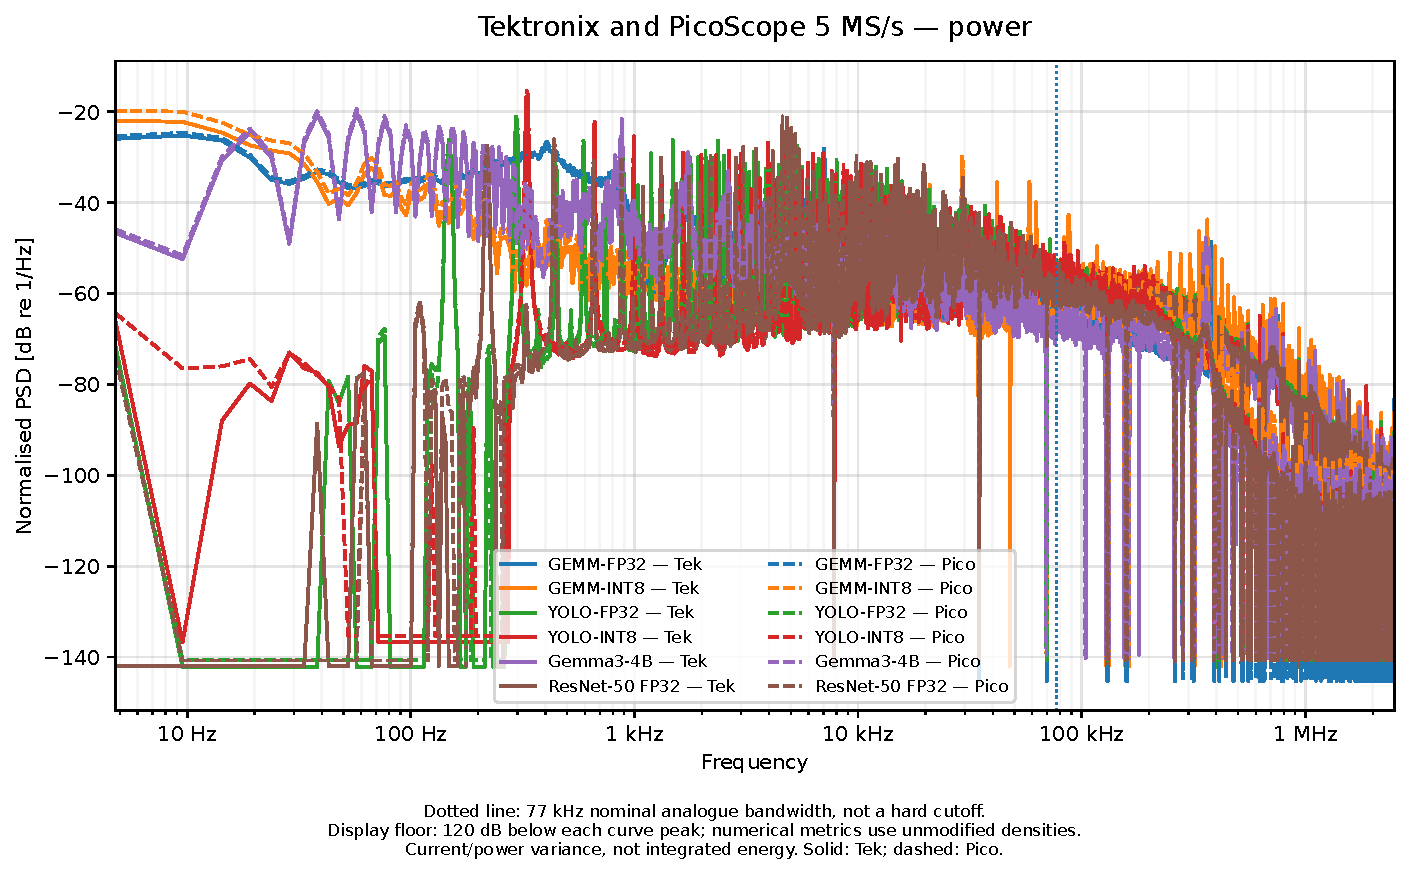
\includegraphics[width=\linewidth]{pico_vs_tek_psd/figures/tek_vs_pico_power_normalised_psd_overlay.pdf}
\caption{Dotted line: 77 kHz nominal analogue bandwidth, not a hard cutoff.
Display floor: 120 dB below each curve peak; numerical metrics use unmodified densities.
Current/power variance, not integrated energy. Solid: Tek; dashed: Pico.}
\label{fig:journal-pico-vs-tek-psd-figures-tek-vs-pico-power-normalised-psd-overlay}
\end{figure}

\begin{figure}[tbp]
\centering
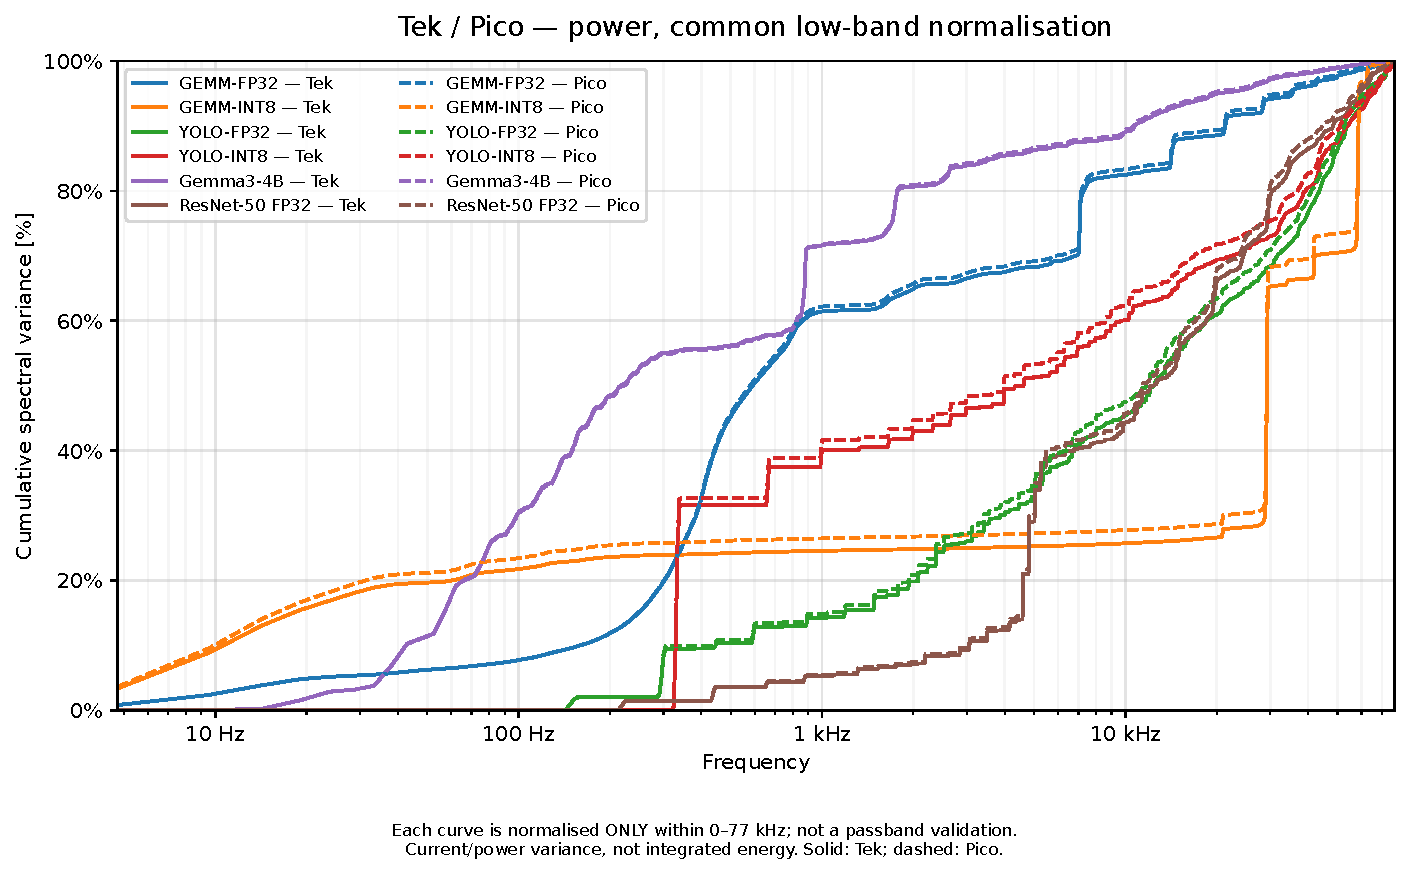
\includegraphics[width=\linewidth]{pico_vs_tek_psd/figures/tek_vs_pico_power_conditional_cumulative_0_77khz.pdf}
\caption{Each curve is normalised ONLY within 0--77 kHz; not a passband validation.
Current/power variance, not integrated energy. Solid: Tek; dashed: Pico.}
\label{fig:journal-pico-vs-tek-psd-figures-tek-vs-pico-power-conditional-cumulative-0-77khz}
\end{figure}

\begin{figure}[tbp]
\centering
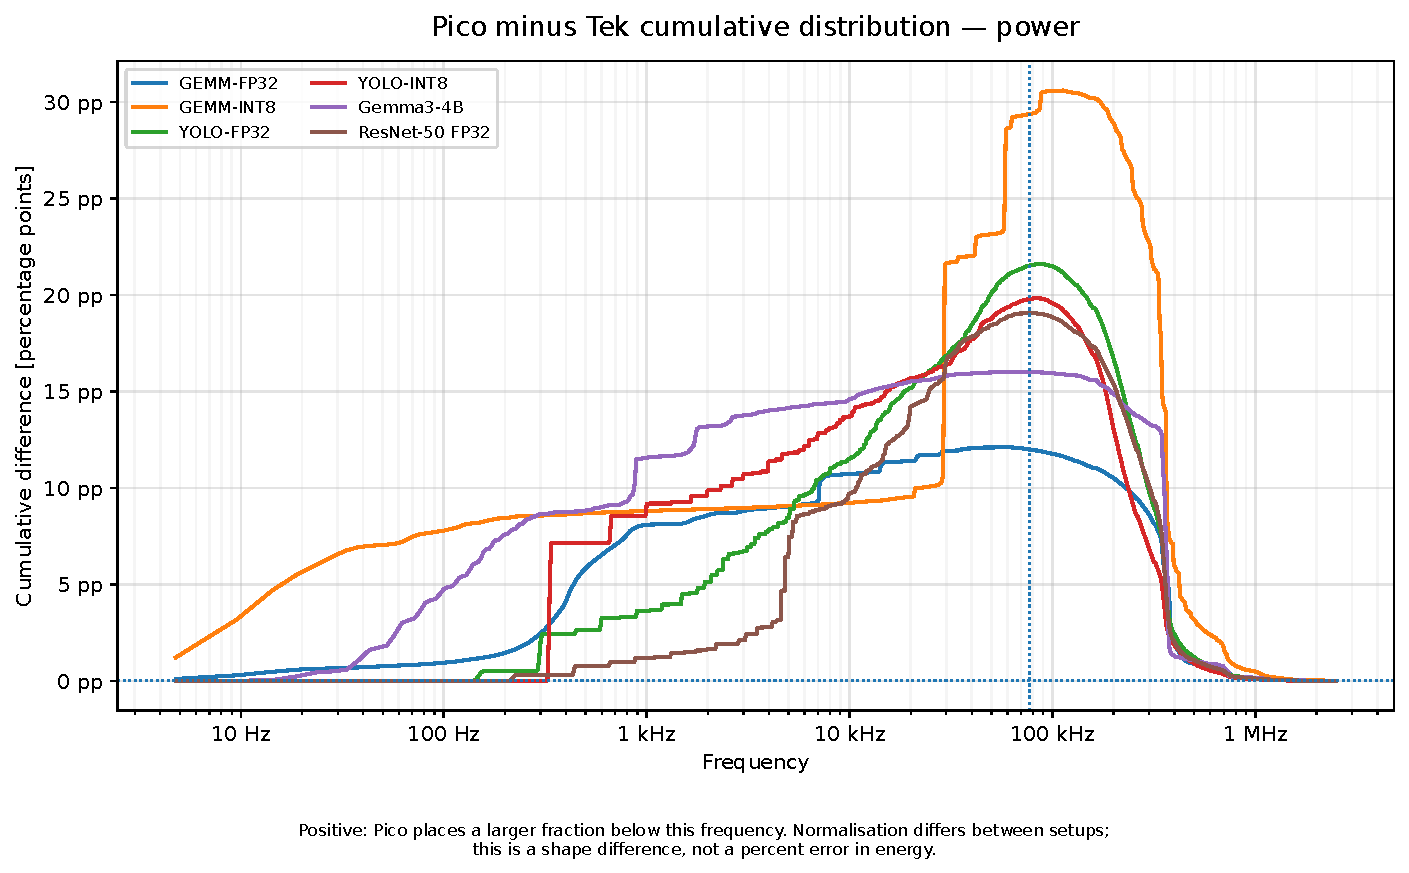
\includegraphics[width=\linewidth]{pico_vs_tek_psd/figures/tek_vs_pico_power_cumulative_difference.pdf}
\caption{Positive: Pico places a larger fraction below this frequency. Normalisation differs between setups;
this is a shape difference, not a percent error in energy.}
\label{fig:journal-pico-vs-tek-psd-figures-tek-vs-pico-power-cumulative-difference}
\end{figure}

\begin{figure}[tbp]
\centering
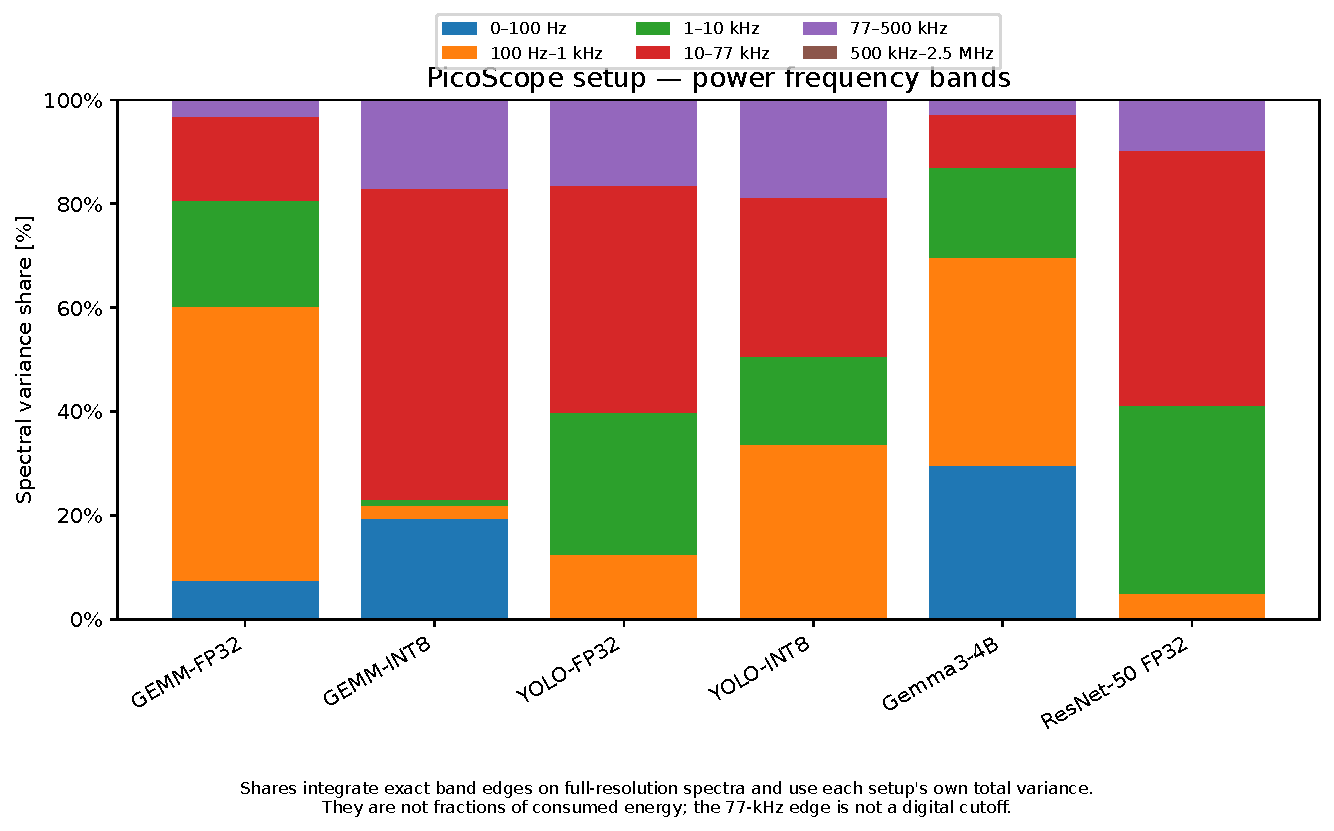
\includegraphics[width=\linewidth]{pico_vs_tek_psd/figures/pico_power_frequency_bands.pdf}
\caption{Shares integrate exact band edges on full-resolution spectra and use each setup's own total variance.
They are not fractions of consumed energy; the 77-kHz edge is not a digital cutoff.}
\label{fig:journal-pico-vs-tek-psd-figures-pico-power-frequency-bands}
\end{figure}

\begin{figure}[tbp]
\centering
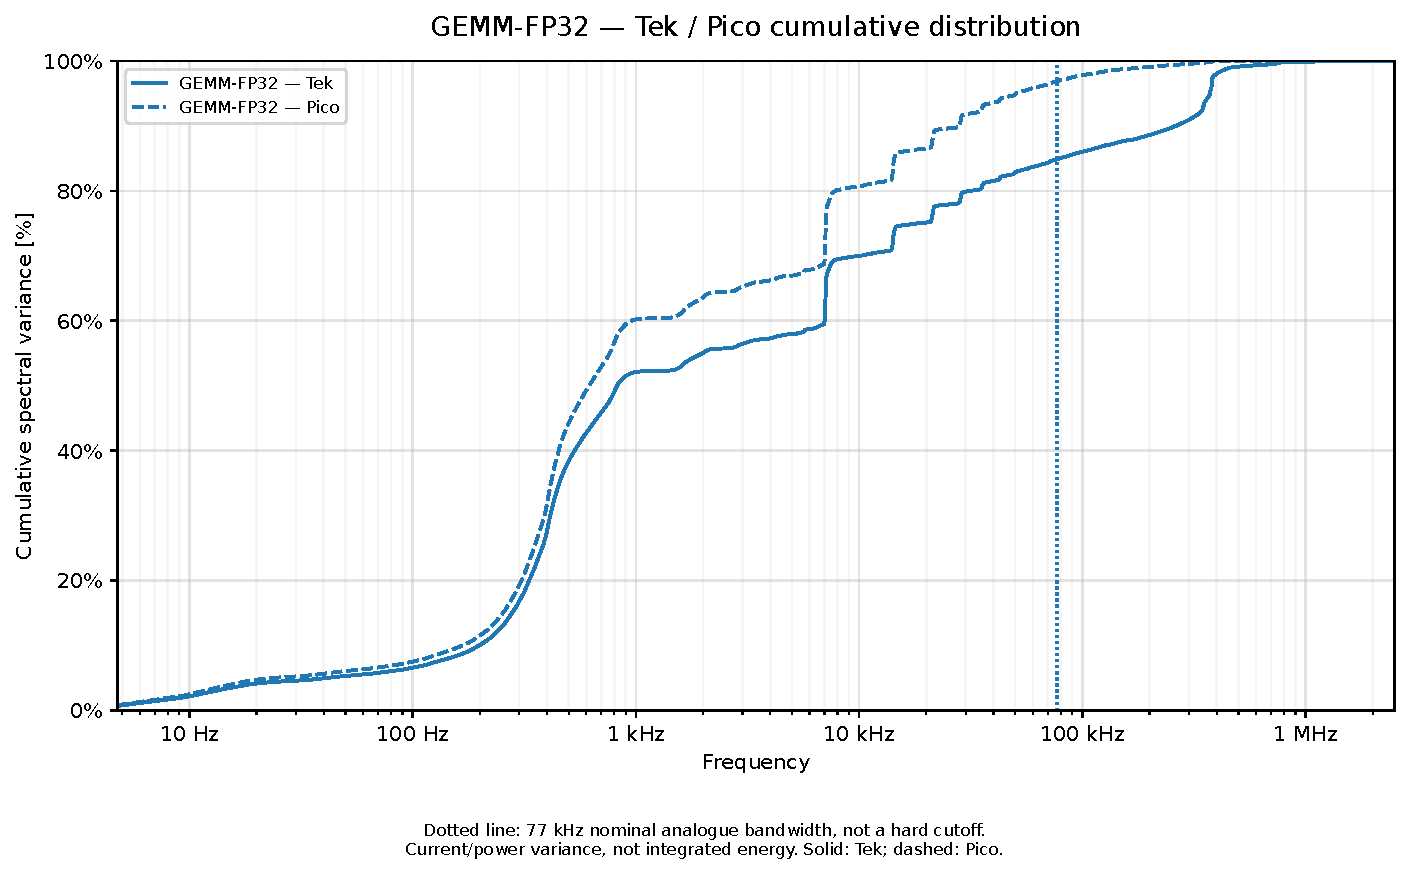
\includegraphics[width=\linewidth]{pico_vs_tek_psd/figures/per_workload/gemmfp32/power_cumulative.pdf}
\caption{Dotted line: 77 kHz nominal analogue bandwidth, not a hard cutoff.
Current/power variance, not integrated energy. Solid: Tek; dashed: Pico.}
\label{fig:journal-pico-vs-tek-psd-figures-per-workload-gemmfp32-power-cumulative}
\end{figure}

\begin{figure}[tbp]
\centering
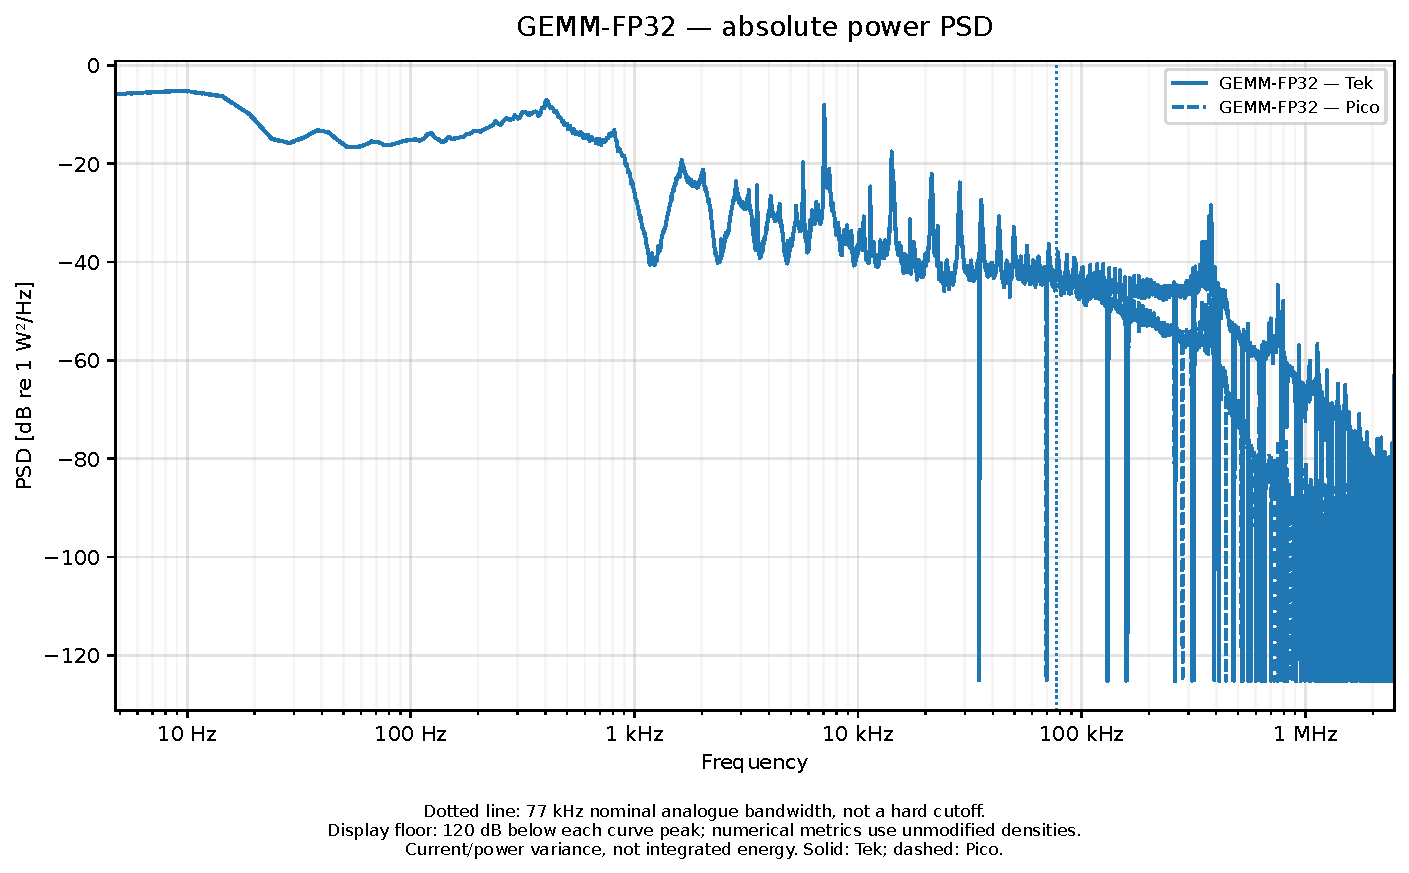
\includegraphics[width=\linewidth]{pico_vs_tek_psd/figures/per_workload/gemmfp32/power_absolute_psd.pdf}
\caption{Dotted line: 77 kHz nominal analogue bandwidth, not a hard cutoff.
Display floor: 120 dB below each curve peak; numerical metrics use unmodified densities.
Current/power variance, not integrated energy. Solid: Tek; dashed: Pico.}
\label{fig:journal-pico-vs-tek-psd-figures-per-workload-gemmfp32-power-absolute-psd}
\end{figure}

\begin{figure}[tbp]
\centering
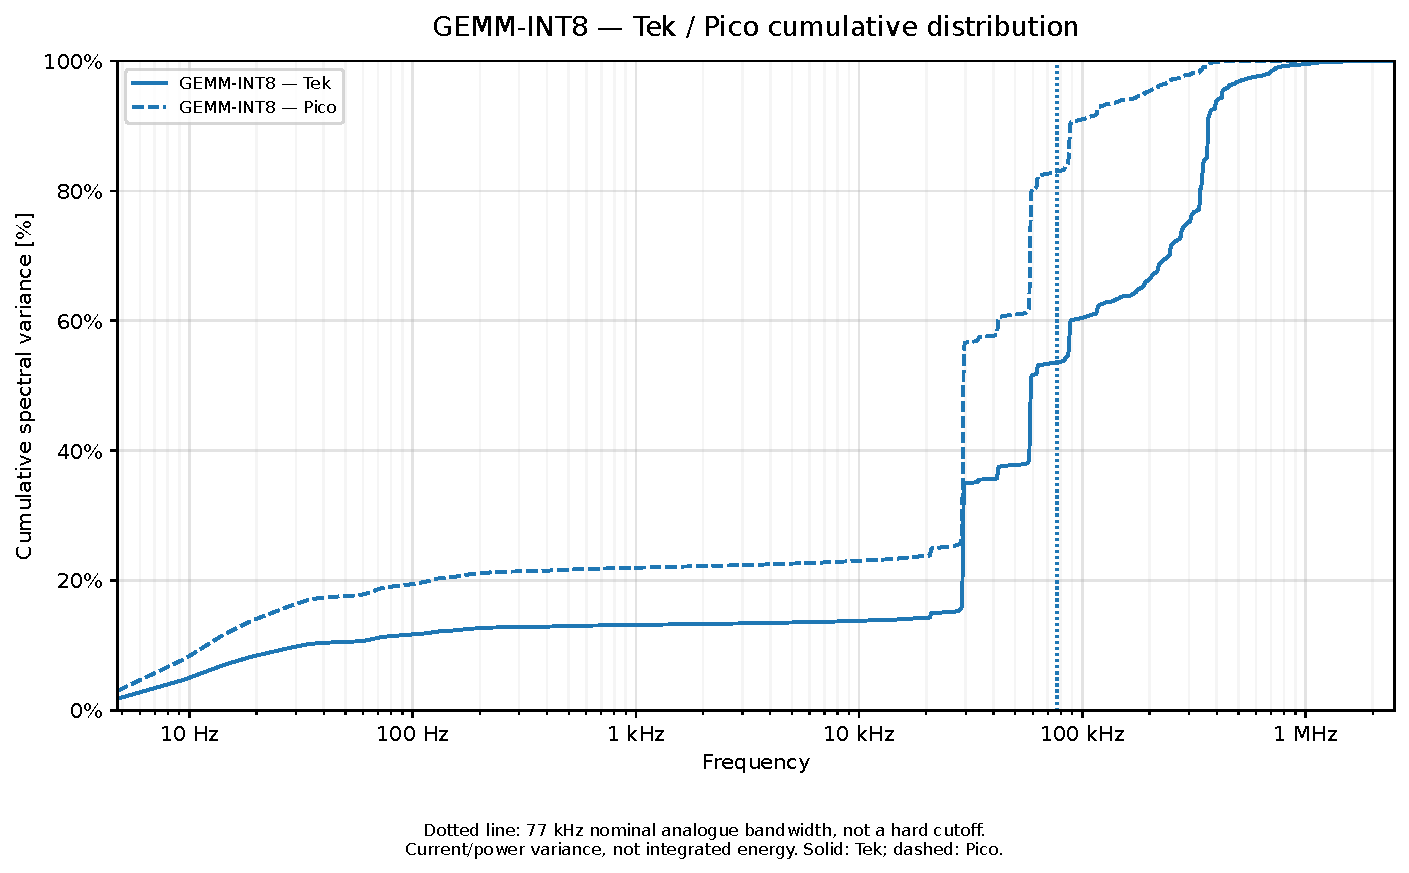
\includegraphics[width=\linewidth]{pico_vs_tek_psd/figures/per_workload/gemmint8/power_cumulative.pdf}
\caption{Dotted line: 77 kHz nominal analogue bandwidth, not a hard cutoff.
Current/power variance, not integrated energy. Solid: Tek; dashed: Pico.}
\label{fig:journal-pico-vs-tek-psd-figures-per-workload-gemmint8-power-cumulative}
\end{figure}

\begin{figure}[tbp]
\centering
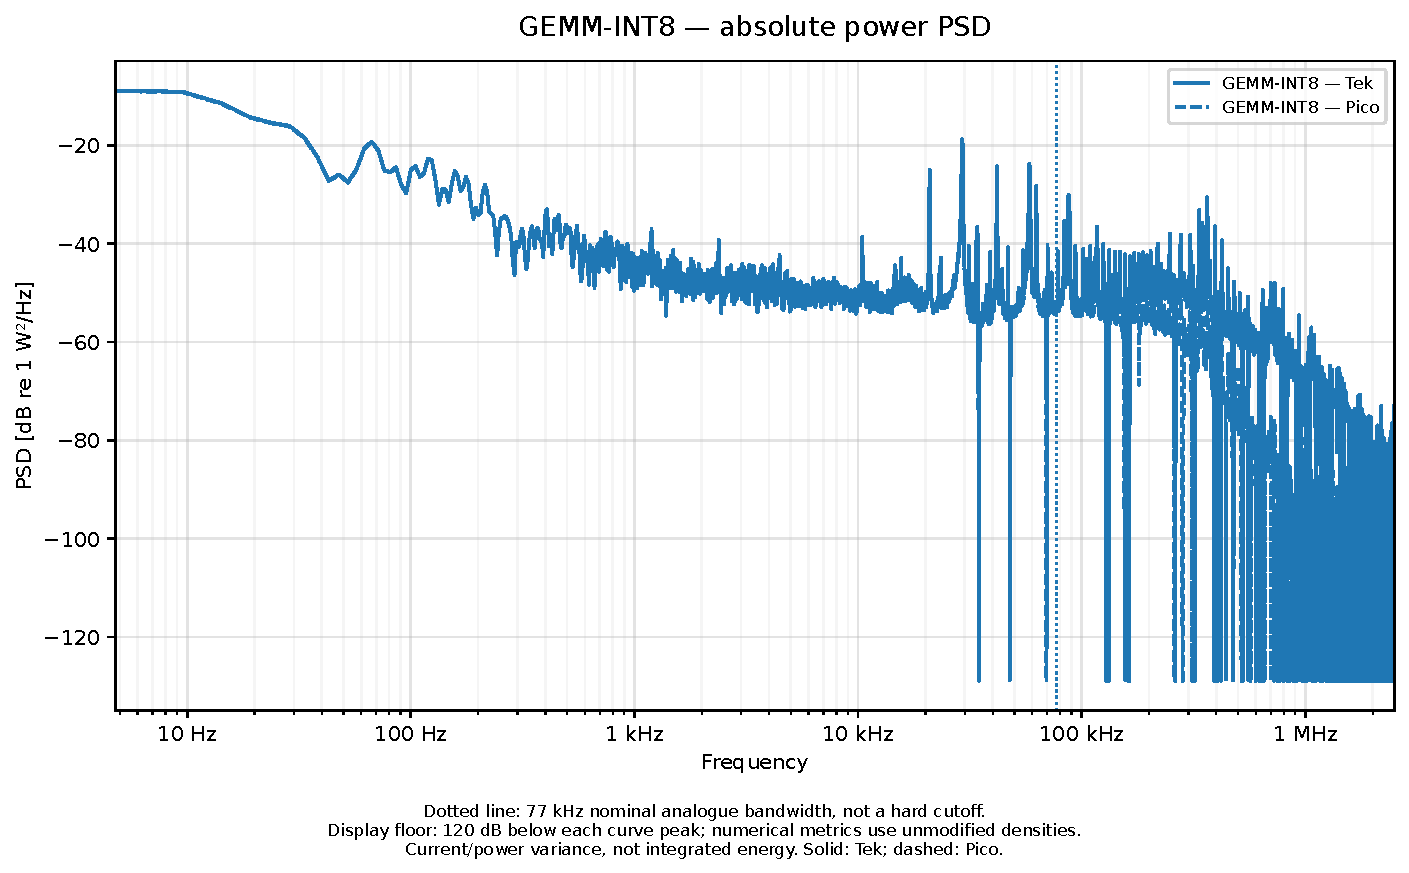
\includegraphics[width=\linewidth]{pico_vs_tek_psd/figures/per_workload/gemmint8/power_absolute_psd.pdf}
\caption{Dotted line: 77 kHz nominal analogue bandwidth, not a hard cutoff.
Display floor: 120 dB below each curve peak; numerical metrics use unmodified densities.
Current/power variance, not integrated energy. Solid: Tek; dashed: Pico.}
\label{fig:journal-pico-vs-tek-psd-figures-per-workload-gemmint8-power-absolute-psd}
\end{figure}

\begin{figure}[tbp]
\centering
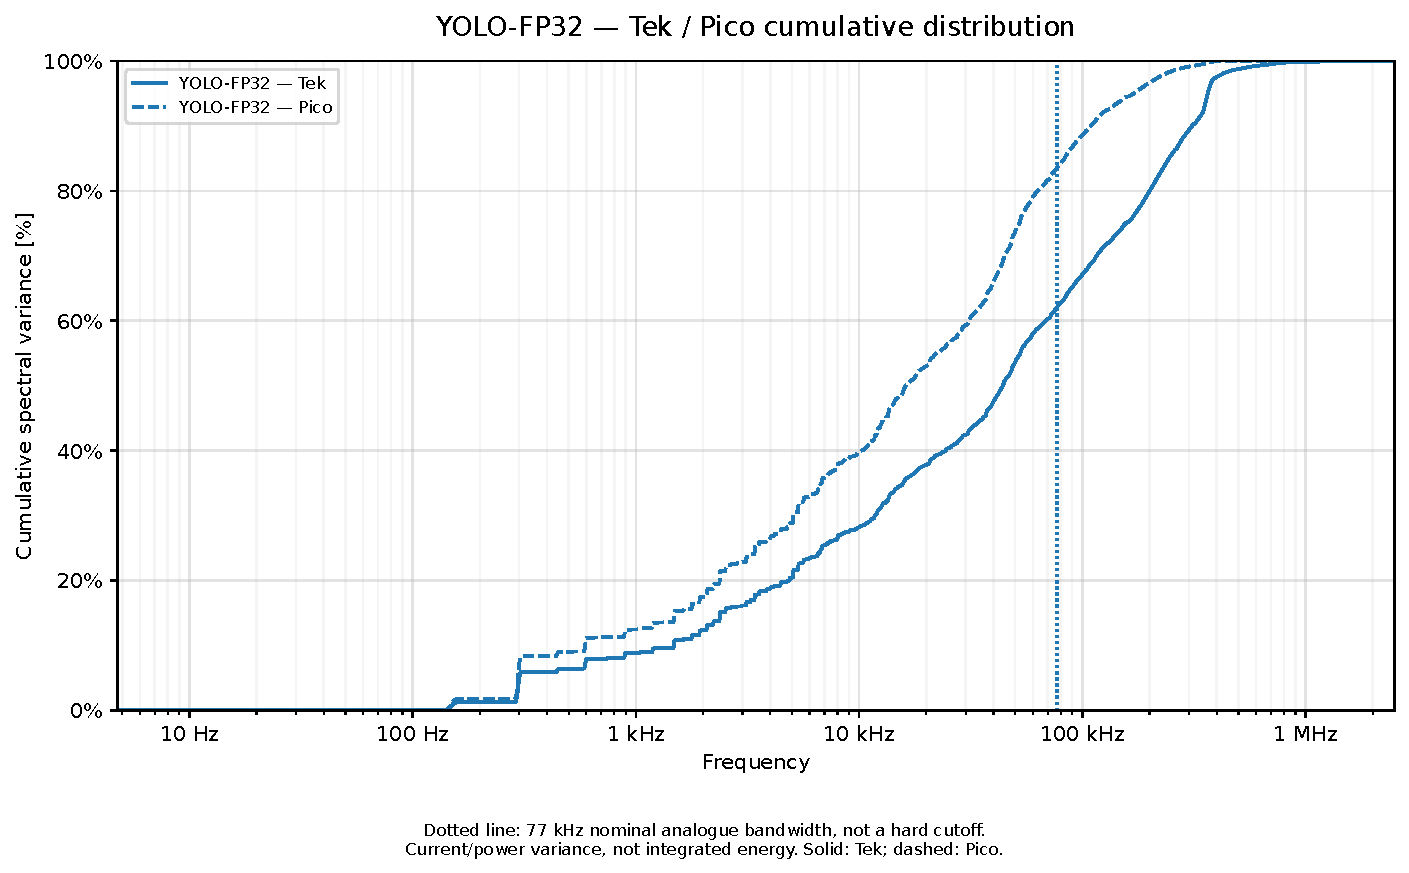
\includegraphics[width=\linewidth]{pico_vs_tek_psd/figures/per_workload/yolofp32/power_cumulative.pdf}
\caption{Dotted line: 77 kHz nominal analogue bandwidth, not a hard cutoff.
Current/power variance, not integrated energy. Solid: Tek; dashed: Pico.}
\label{fig:journal-pico-vs-tek-psd-figures-per-workload-yolofp32-power-cumulative}
\end{figure}

\begin{figure}[tbp]
\centering
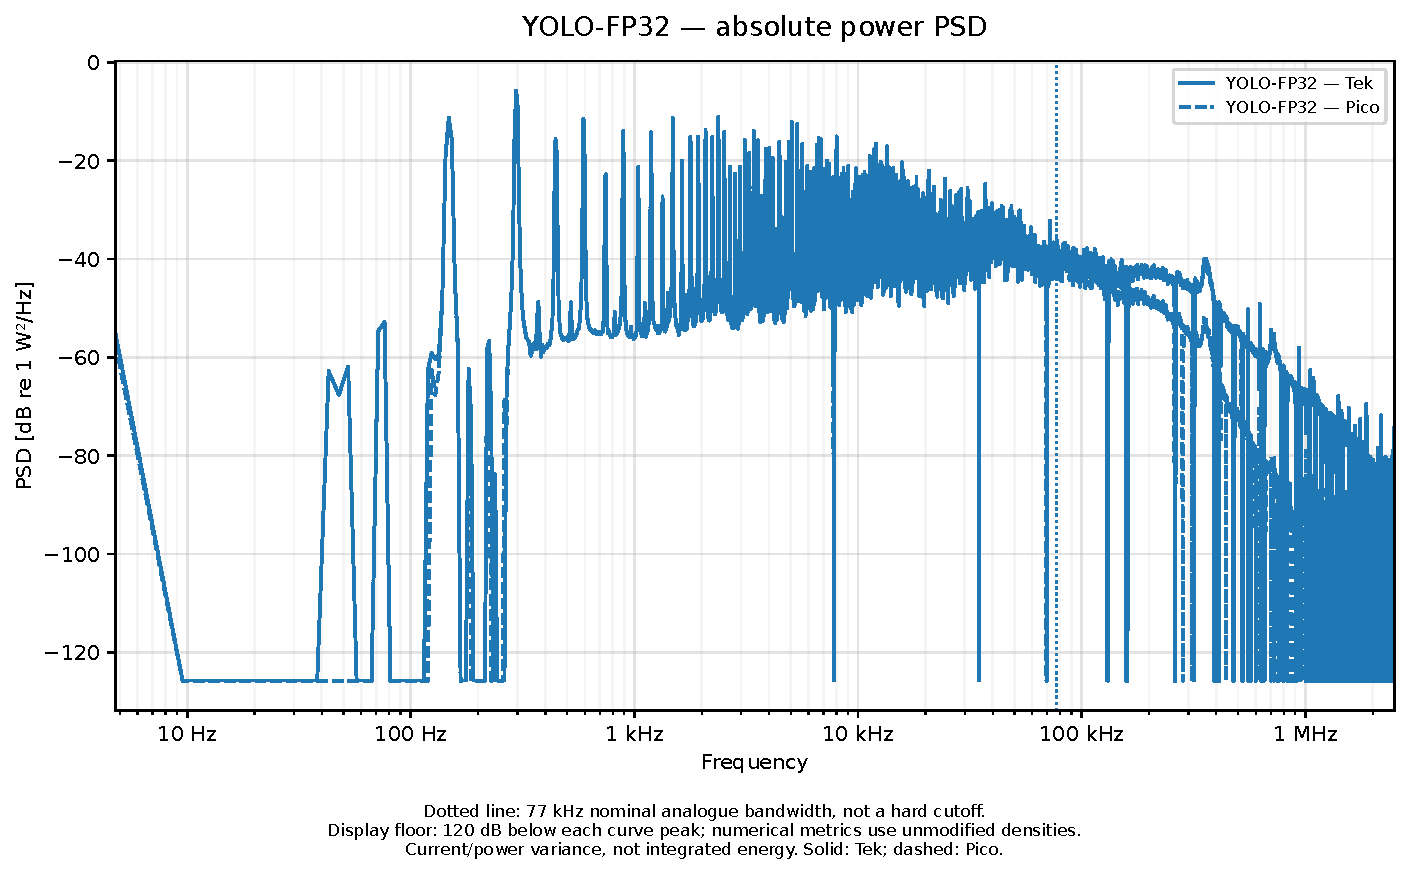
\includegraphics[width=\linewidth]{pico_vs_tek_psd/figures/per_workload/yolofp32/power_absolute_psd.pdf}
\caption{Dotted line: 77 kHz nominal analogue bandwidth, not a hard cutoff.
Display floor: 120 dB below each curve peak; numerical metrics use unmodified densities.
Current/power variance, not integrated energy. Solid: Tek; dashed: Pico.}
\label{fig:journal-pico-vs-tek-psd-figures-per-workload-yolofp32-power-absolute-psd}
\end{figure}

\begin{figure}[tbp]
\centering
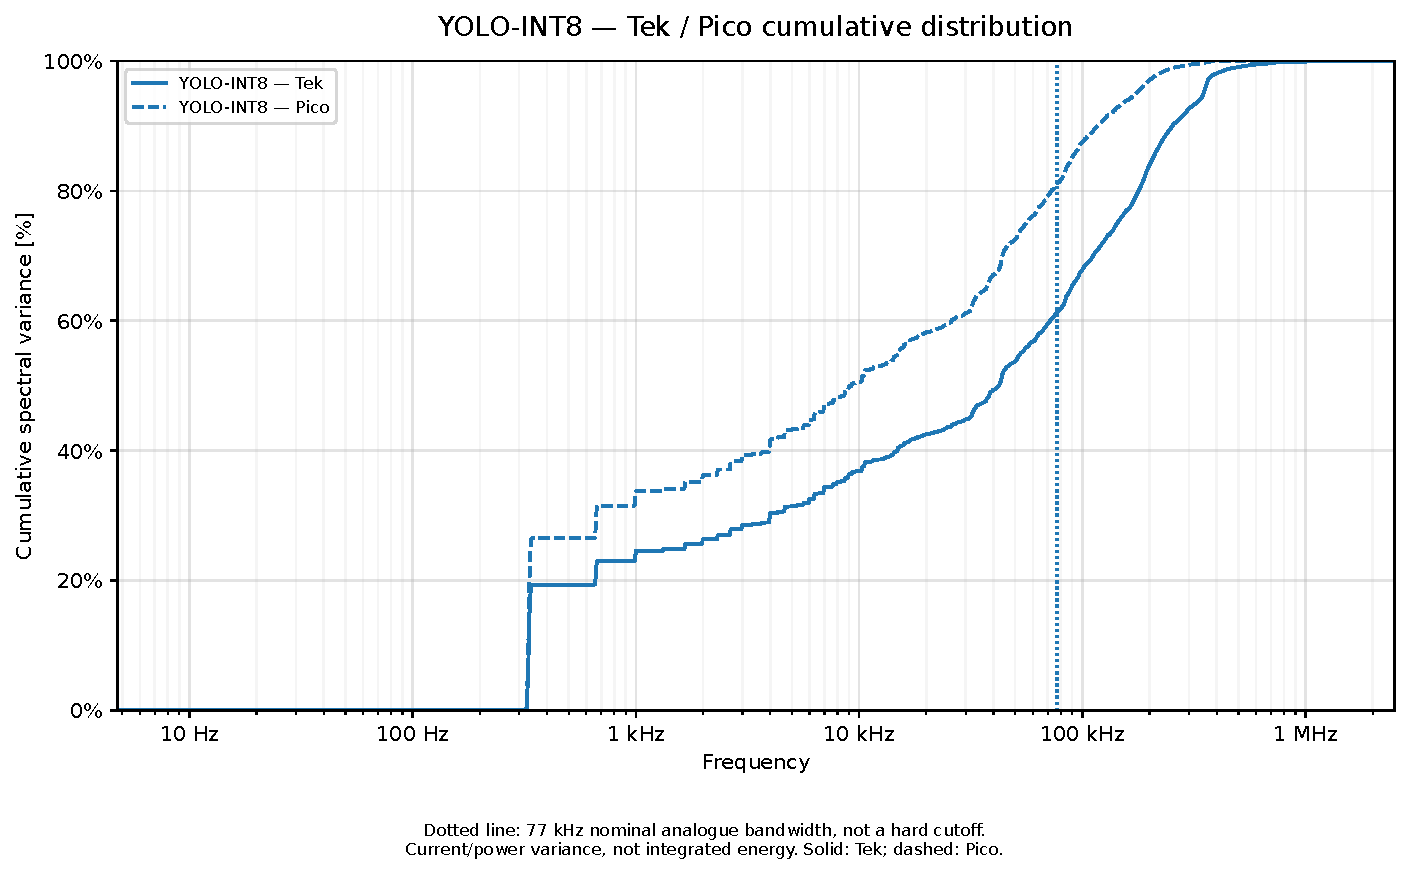
\includegraphics[width=\linewidth]{pico_vs_tek_psd/figures/per_workload/yoloint8/power_cumulative.pdf}
\caption{Dotted line: 77 kHz nominal analogue bandwidth, not a hard cutoff.
Current/power variance, not integrated energy. Solid: Tek; dashed: Pico.}
\label{fig:journal-pico-vs-tek-psd-figures-per-workload-yoloint8-power-cumulative}
\end{figure}

\begin{figure}[tbp]
\centering
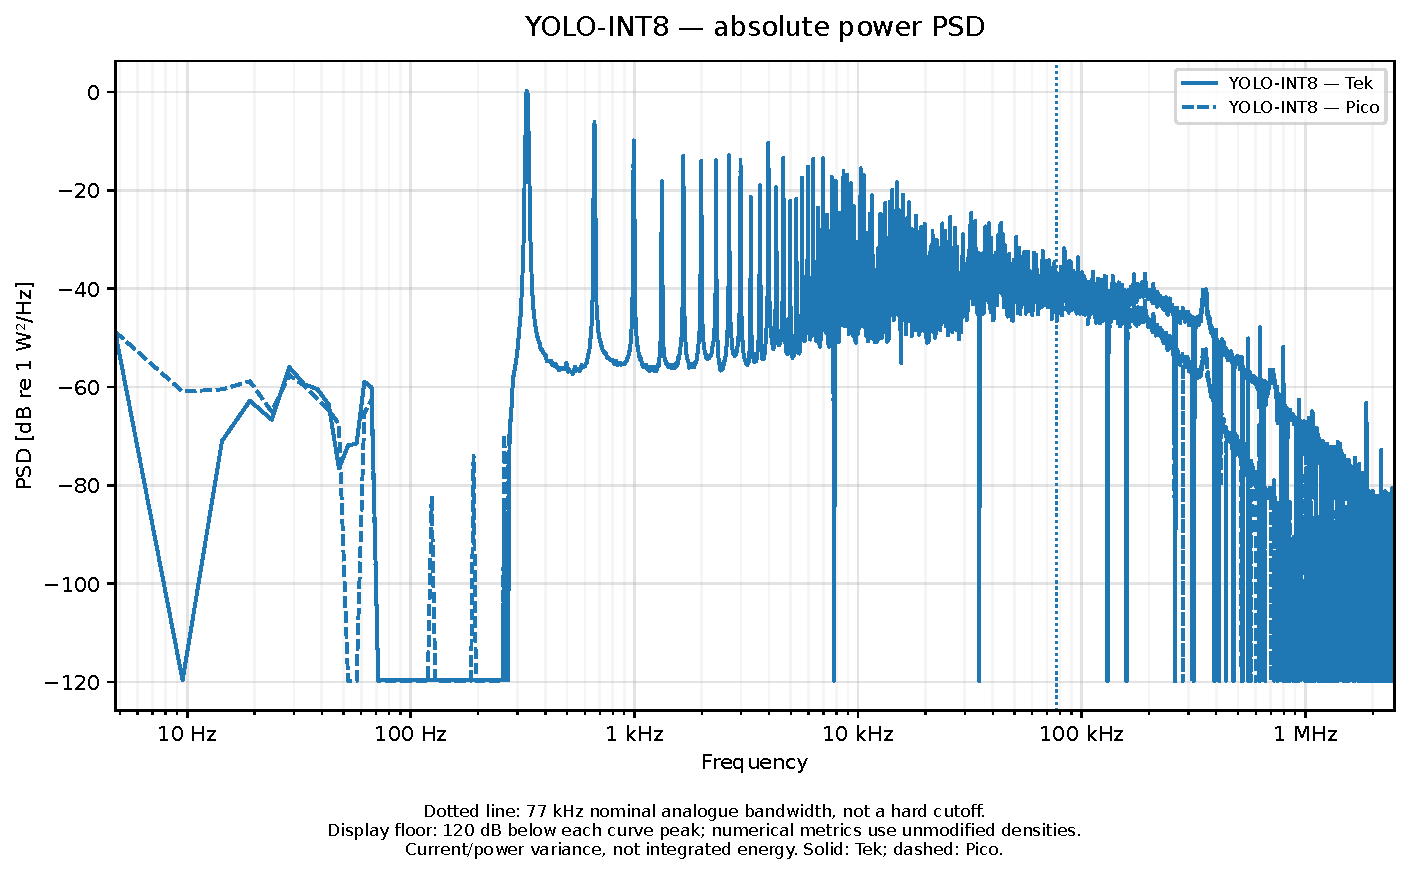
\includegraphics[width=\linewidth]{pico_vs_tek_psd/figures/per_workload/yoloint8/power_absolute_psd.pdf}
\caption{Dotted line: 77 kHz nominal analogue bandwidth, not a hard cutoff.
Display floor: 120 dB below each curve peak; numerical metrics use unmodified densities.
Current/power variance, not integrated energy. Solid: Tek; dashed: Pico.}
\label{fig:journal-pico-vs-tek-psd-figures-per-workload-yoloint8-power-absolute-psd}
\end{figure}

\begin{figure}[tbp]
\centering
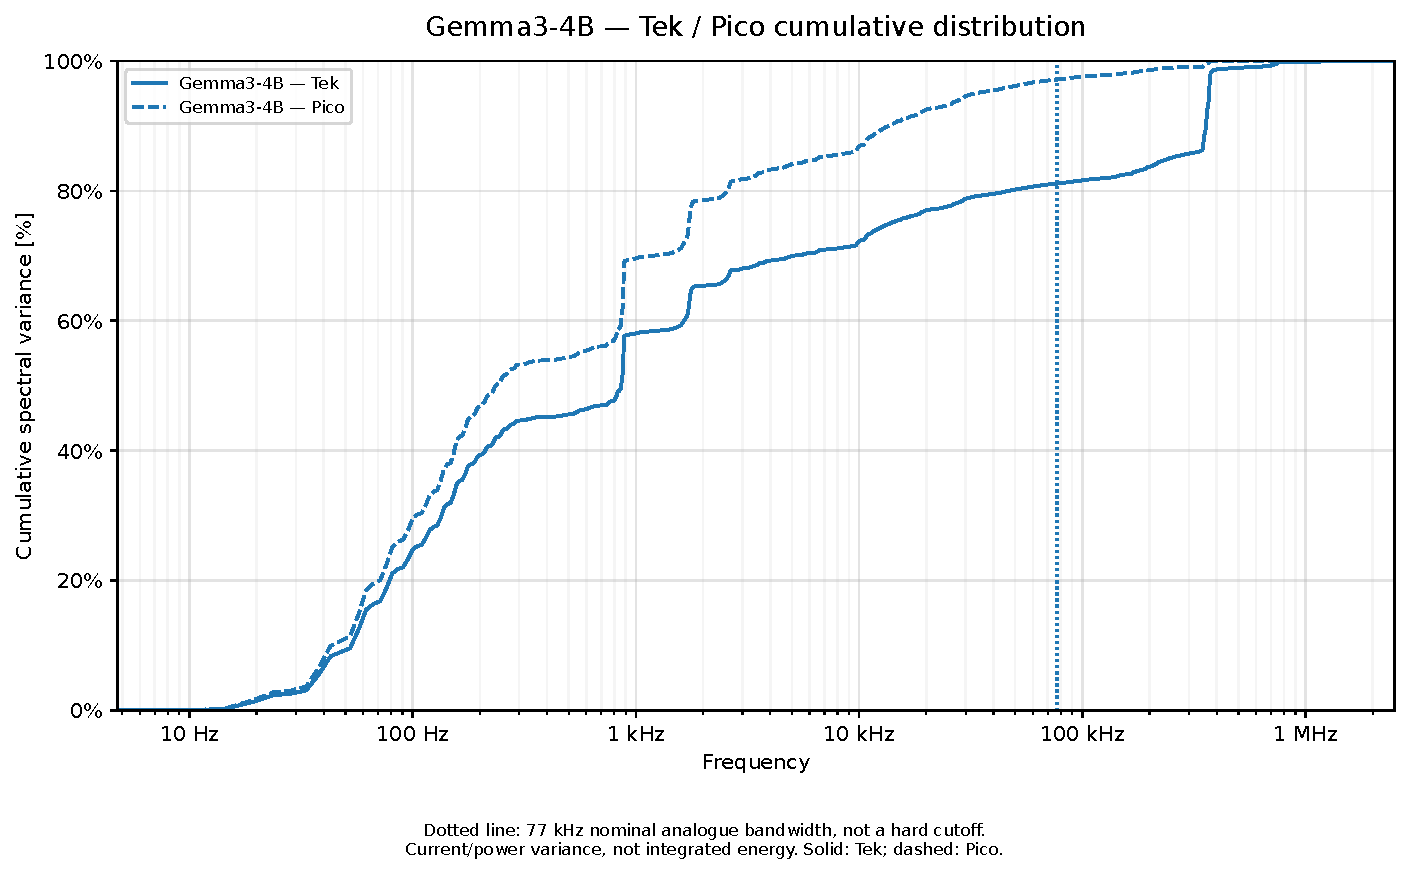
\includegraphics[width=\linewidth]{pico_vs_tek_psd/figures/per_workload/gemma3-4b/power_cumulative.pdf}
\caption{Dotted line: 77 kHz nominal analogue bandwidth, not a hard cutoff.
Current/power variance, not integrated energy. Solid: Tek; dashed: Pico.}
\label{fig:journal-pico-vs-tek-psd-figures-per-workload-gemma3-4b-power-cumulative}
\end{figure}

\begin{figure}[tbp]
\centering
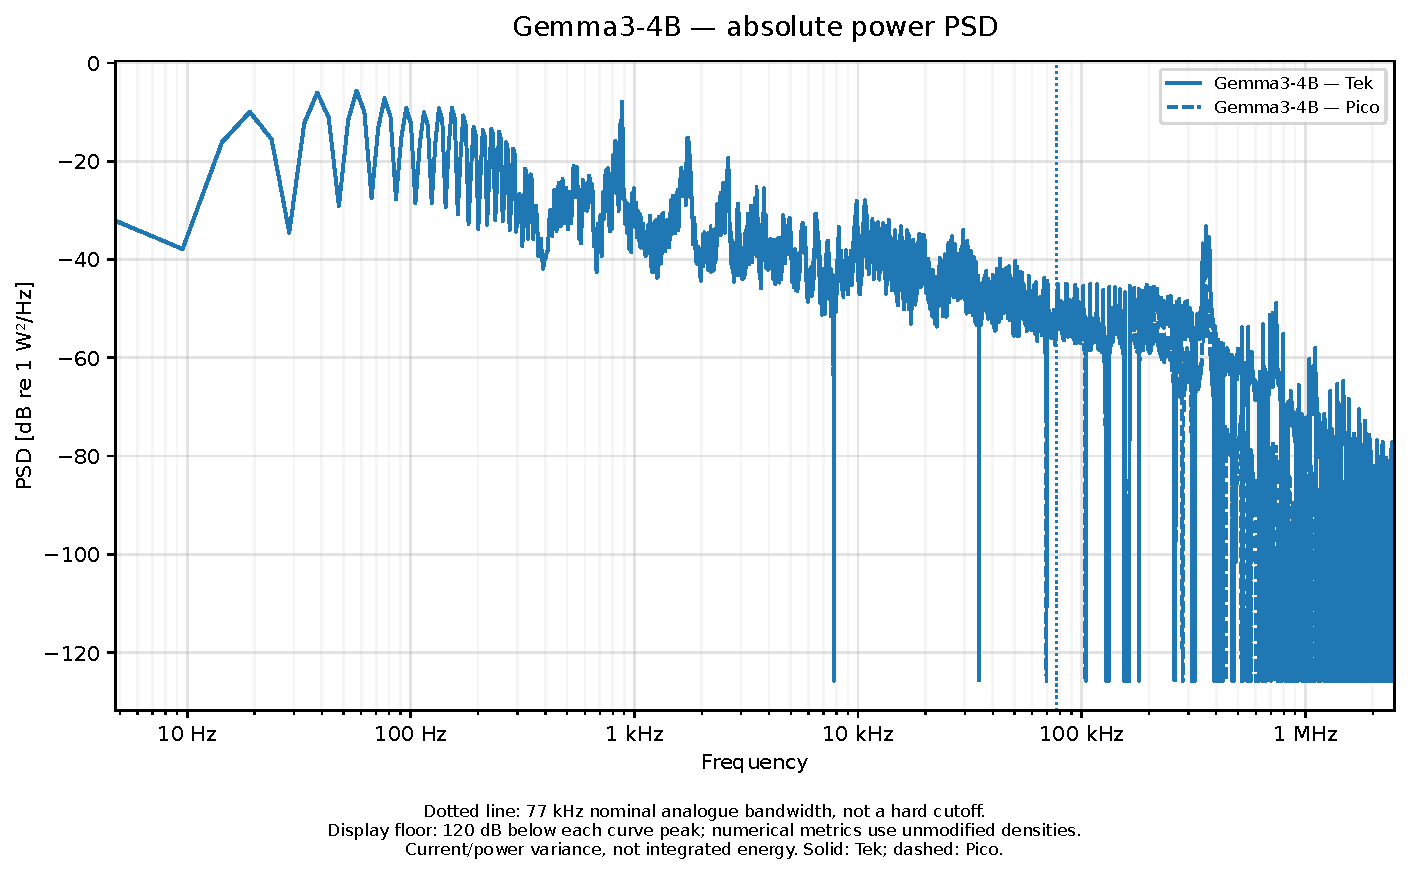
\includegraphics[width=\linewidth]{pico_vs_tek_psd/figures/per_workload/gemma3-4b/power_absolute_psd.pdf}
\caption{Dotted line: 77 kHz nominal analogue bandwidth, not a hard cutoff.
Display floor: 120 dB below each curve peak; numerical metrics use unmodified densities.
Current/power variance, not integrated energy. Solid: Tek; dashed: Pico.}
\label{fig:journal-pico-vs-tek-psd-figures-per-workload-gemma3-4b-power-absolute-psd}
\end{figure}

\begin{figure}[tbp]
\centering
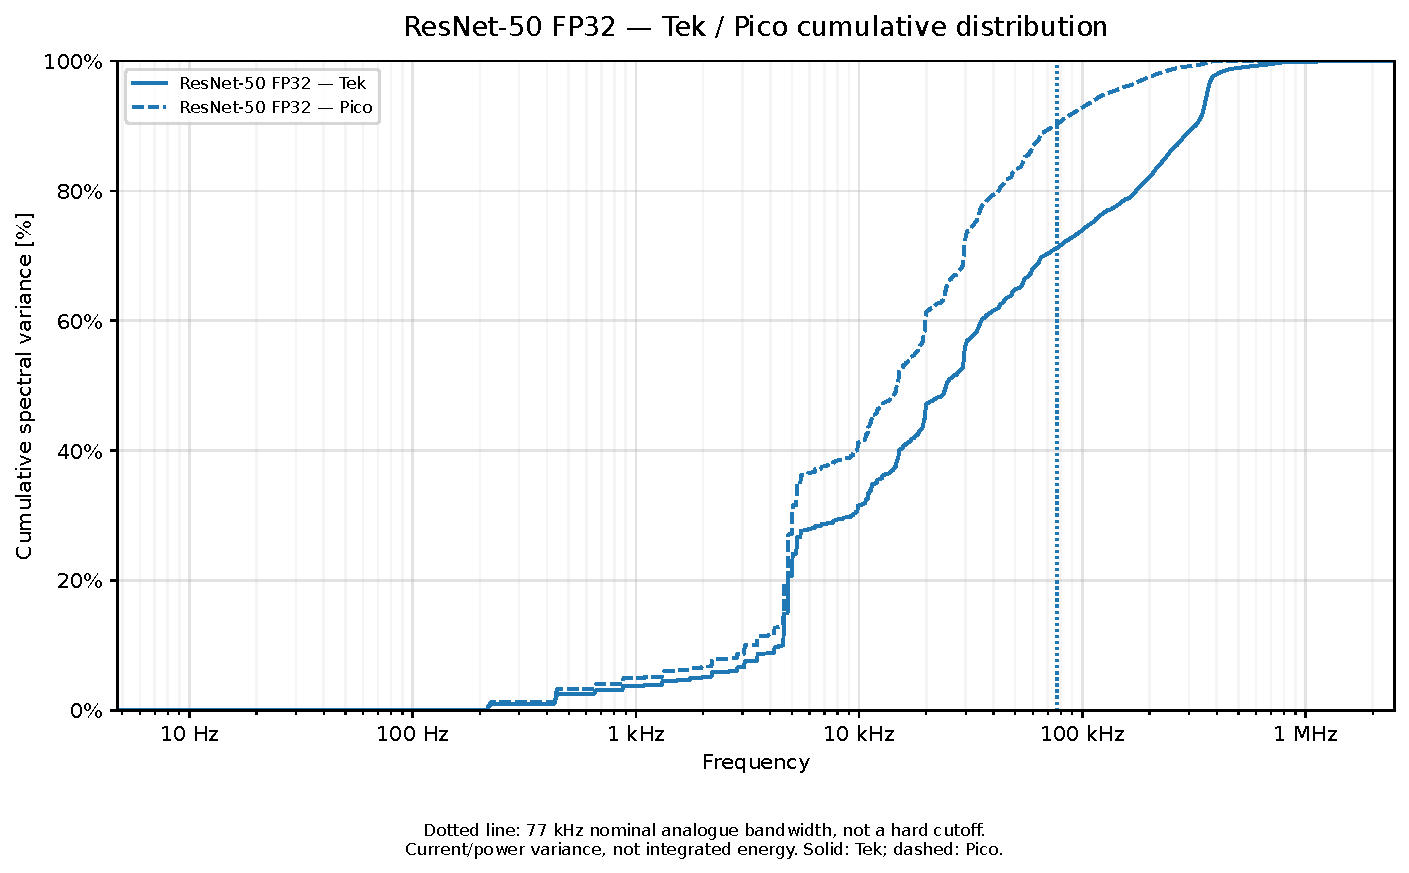
\includegraphics[width=\linewidth]{pico_vs_tek_psd/figures/per_workload/resnet50/power_cumulative.pdf}
\caption{Dotted line: 77 kHz nominal analogue bandwidth, not a hard cutoff.
Current/power variance, not integrated energy. Solid: Tek; dashed: Pico.}
\label{fig:journal-pico-vs-tek-psd-figures-per-workload-resnet50-power-cumulative}
\end{figure}

\begin{figure}[tbp]
\centering
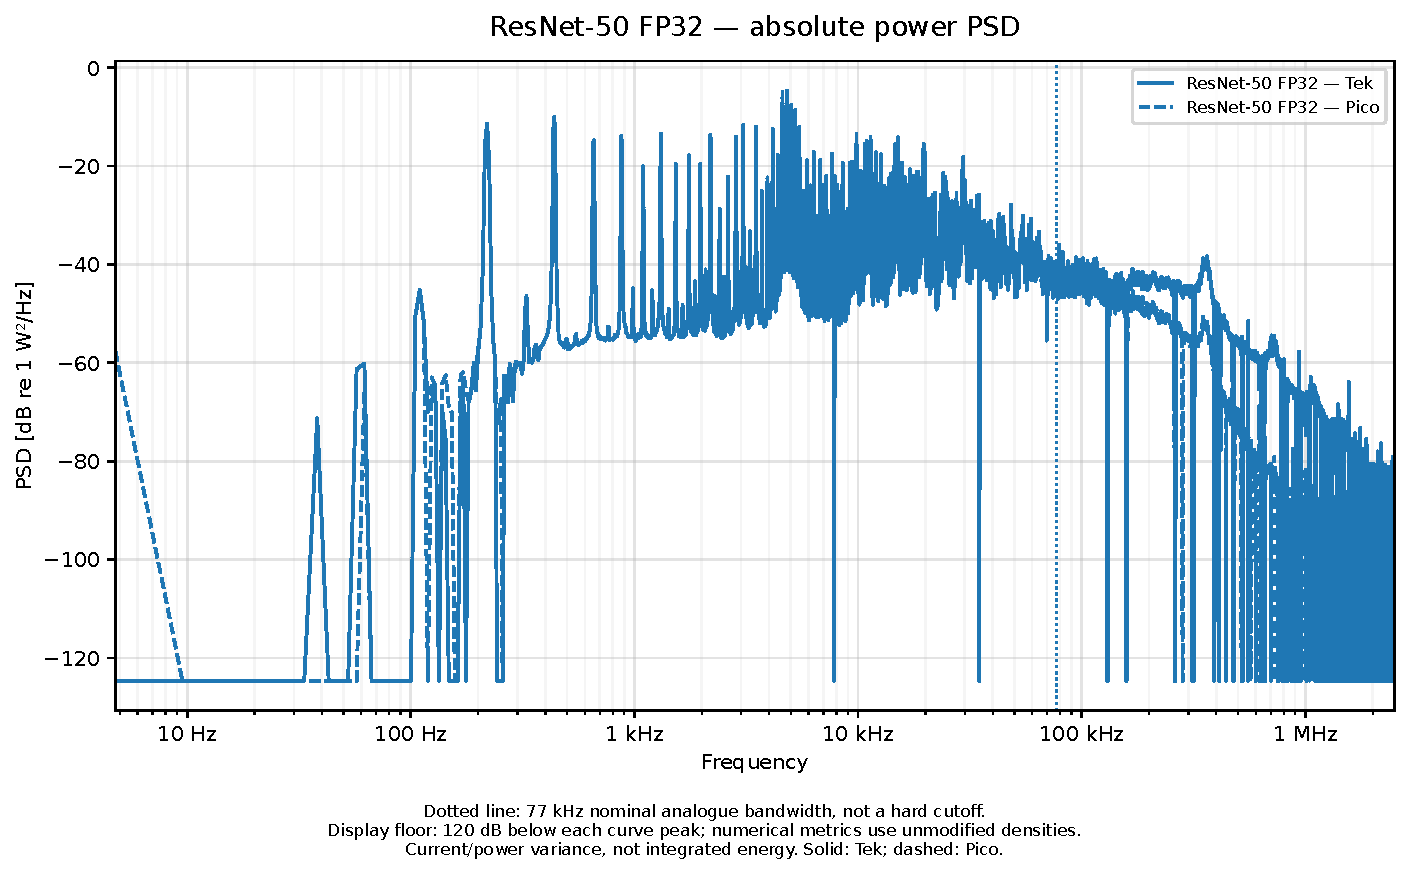
\includegraphics[width=\linewidth]{pico_vs_tek_psd/figures/per_workload/resnet50/power_absolute_psd.pdf}
\caption{Dotted line: 77 kHz nominal analogue bandwidth, not a hard cutoff.
Display floor: 120 dB below each curve peak; numerical metrics use unmodified densities.
Current/power variance, not integrated energy. Solid: Tek; dashed: Pico.}
\label{fig:journal-pico-vs-tek-psd-figures-per-workload-resnet50-power-absolute-psd}
\end{figure}

\begin{figure}[tbp]
\centering
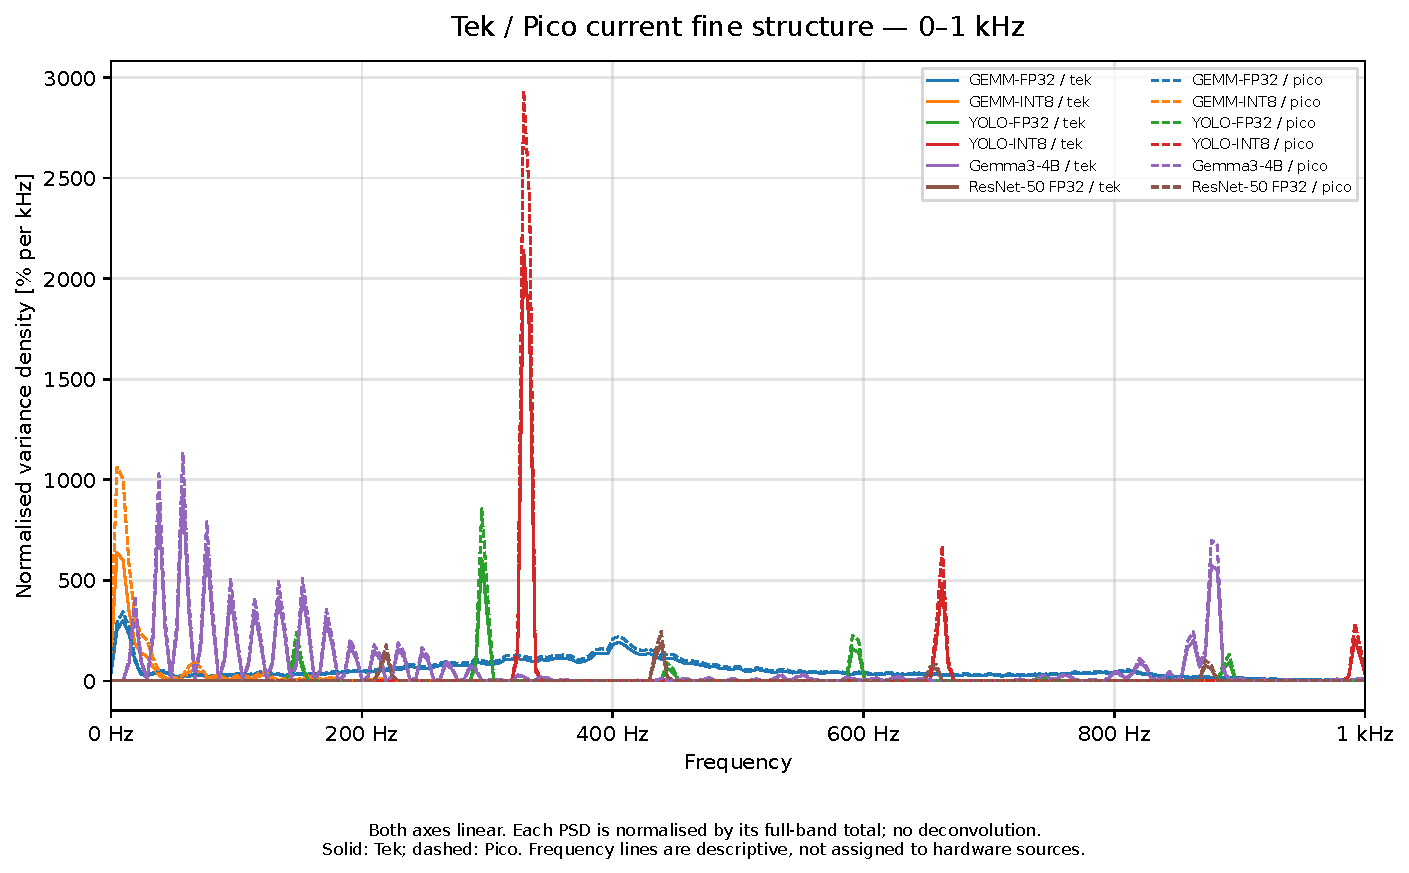
\includegraphics[width=\linewidth]{pico_vs_tek_psd/figures/fine_structure/tek_vs_pico_fine_0_1000hz.pdf}
\caption{Both axes linear. Each PSD is normalised by its full-band total; no deconvolution.
Solid: Tek; dashed: Pico. Frequency lines are descriptive, not assigned to hardware sources.}
\label{fig:journal-pico-vs-tek-psd-figures-fine-structure-tek-vs-pico-fine-0-1000hz}
\end{figure}

\begin{figure}[tbp]
\centering
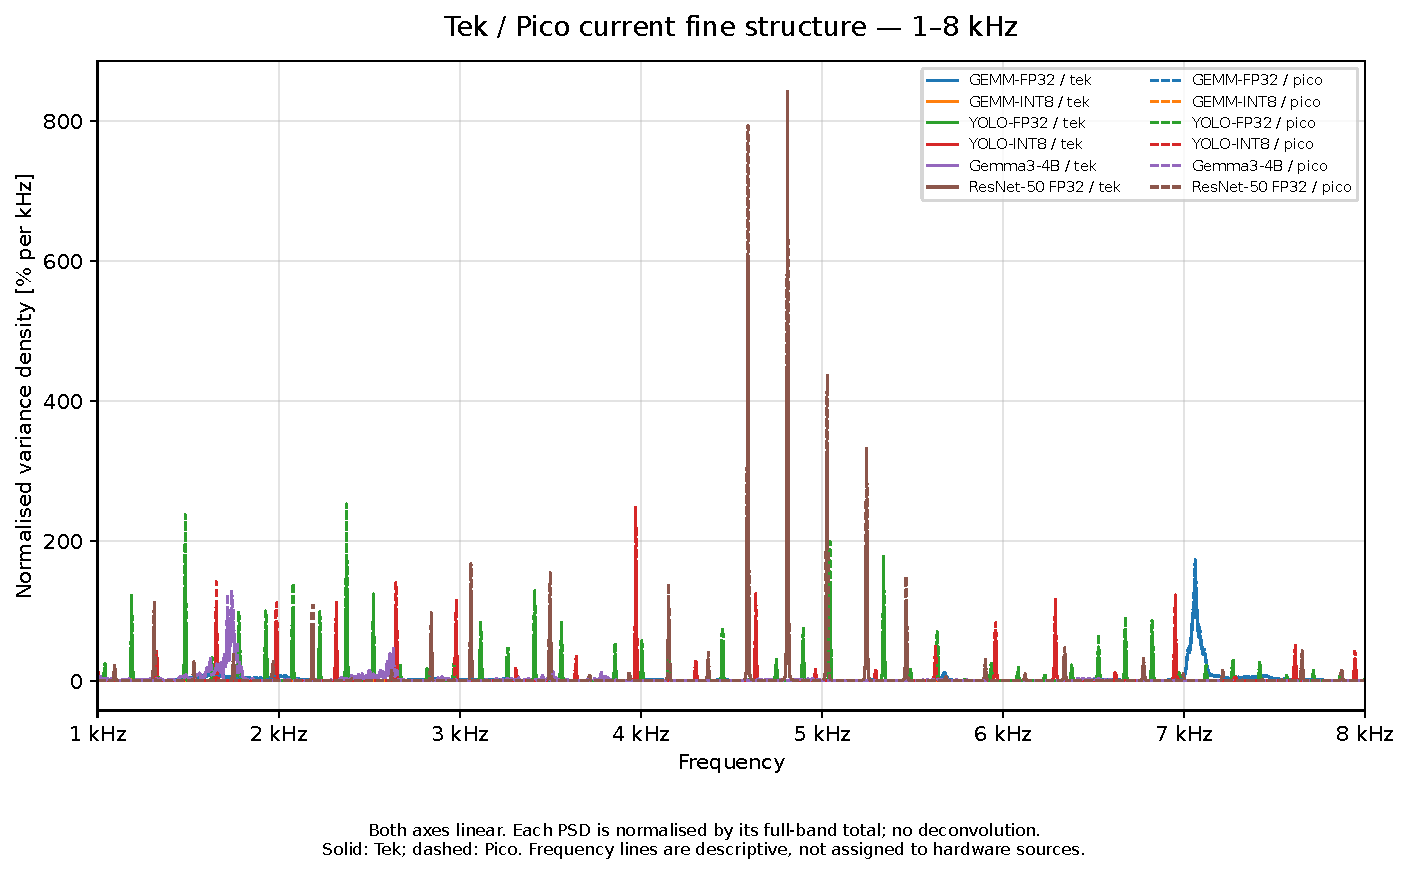
\includegraphics[width=\linewidth]{pico_vs_tek_psd/figures/fine_structure/tek_vs_pico_fine_1000_8000hz.pdf}
\caption{Both axes linear. Each PSD is normalised by its full-band total; no deconvolution.
Solid: Tek; dashed: Pico. Frequency lines are descriptive, not assigned to hardware sources.}
\label{fig:journal-pico-vs-tek-psd-figures-fine-structure-tek-vs-pico-fine-1000-8000hz}
\end{figure}

\begin{figure}[tbp]
\centering
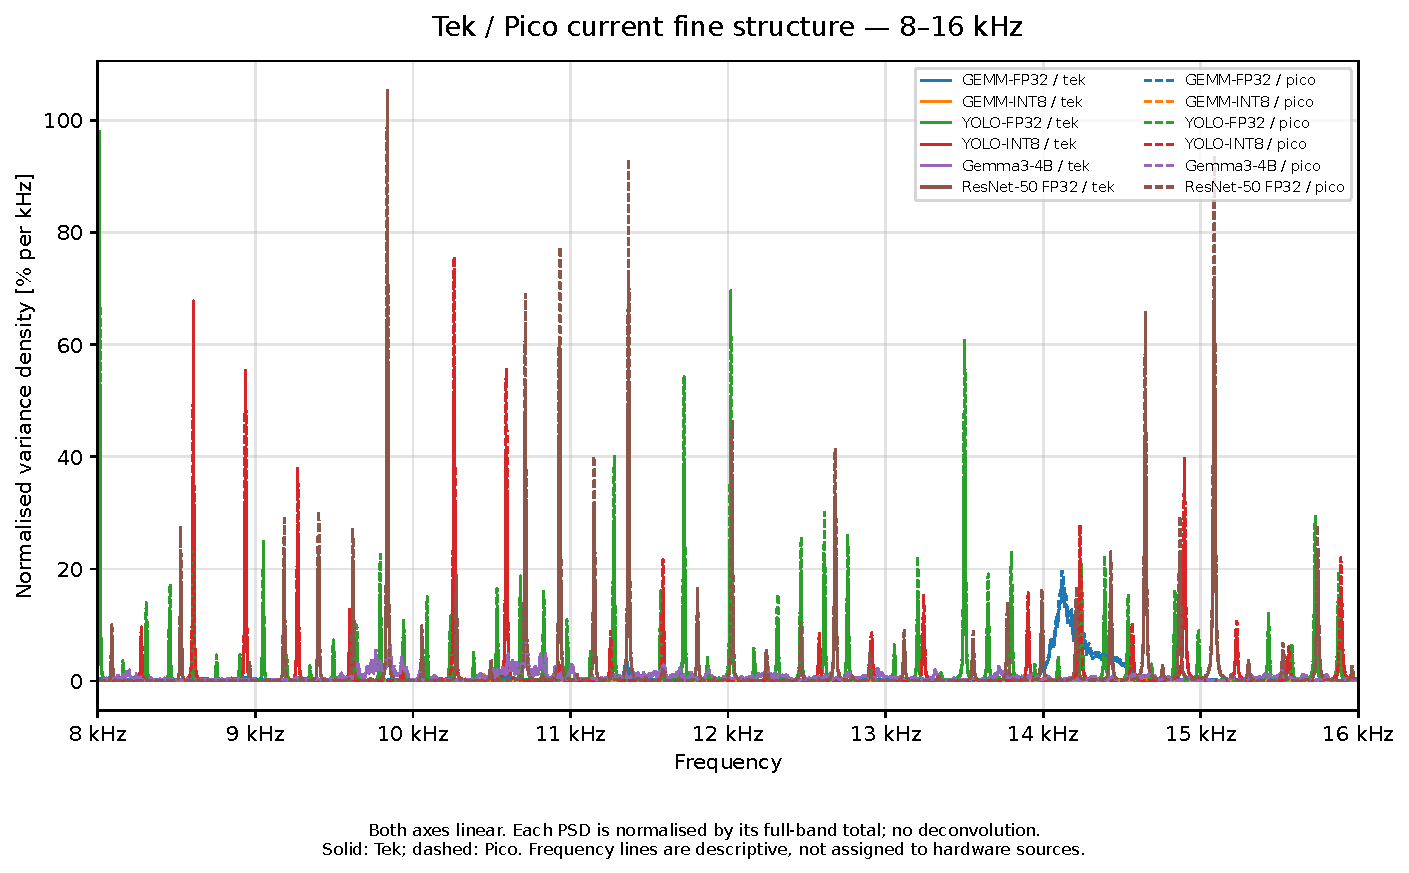
\includegraphics[width=\linewidth]{pico_vs_tek_psd/figures/fine_structure/tek_vs_pico_fine_8000_16000hz.pdf}
\caption{Both axes linear. Each PSD is normalised by its full-band total; no deconvolution.
Solid: Tek; dashed: Pico. Frequency lines are descriptive, not assigned to hardware sources.}
\label{fig:journal-pico-vs-tek-psd-figures-fine-structure-tek-vs-pico-fine-8000-16000hz}
\end{figure}

\begin{figure}[tbp]
\centering
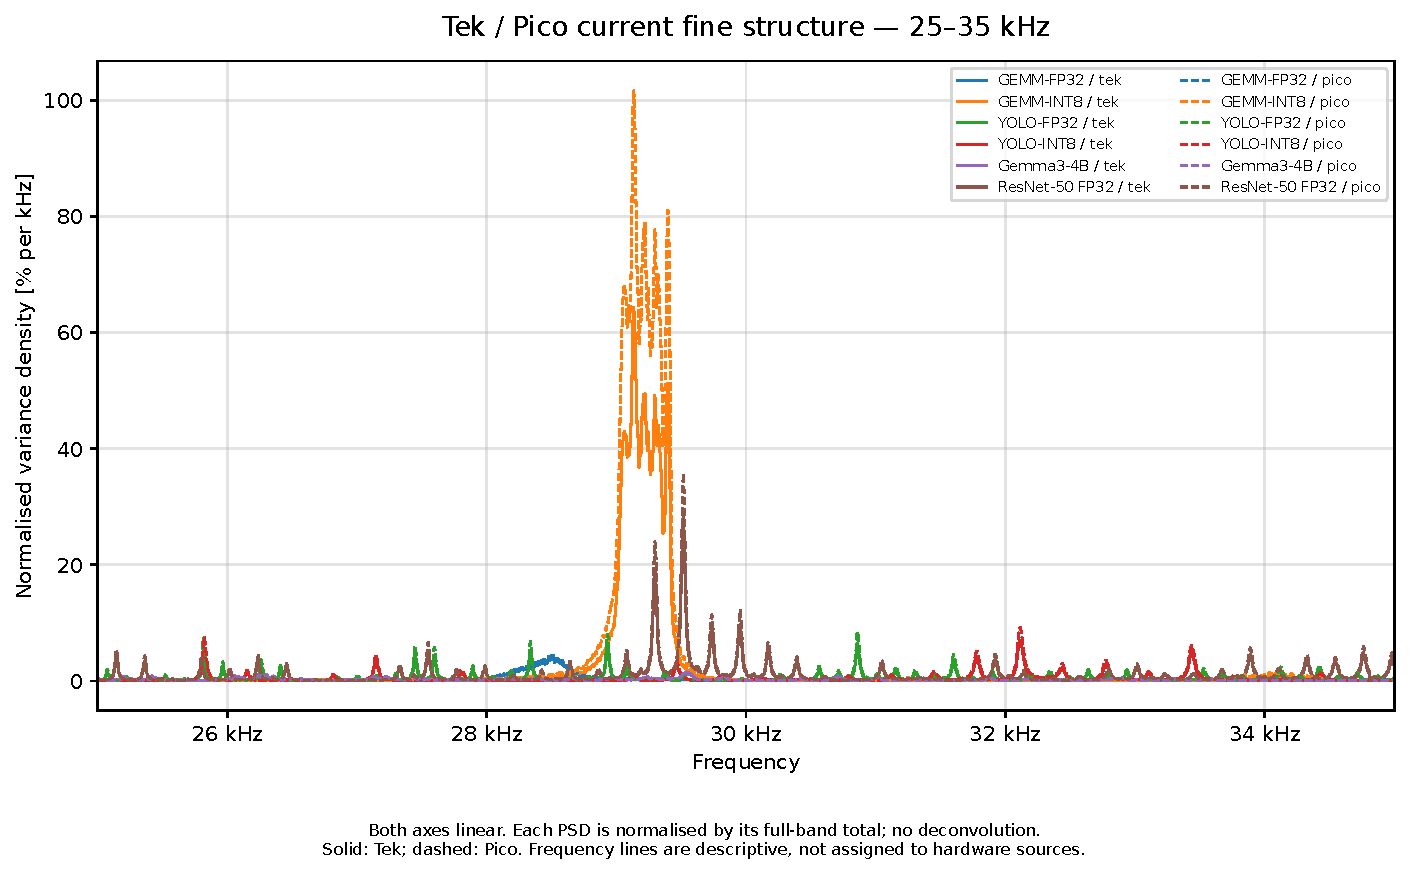
\includegraphics[width=\linewidth]{pico_vs_tek_psd/figures/fine_structure/tek_vs_pico_fine_25000_35000hz.pdf}
\caption{Both axes linear. Each PSD is normalised by its full-band total; no deconvolution.
Solid: Tek; dashed: Pico. Frequency lines are descriptive, not assigned to hardware sources.}
\label{fig:journal-pico-vs-tek-psd-figures-fine-structure-tek-vs-pico-fine-25000-35000hz}
\end{figure}

\begin{figure}[tbp]
\centering
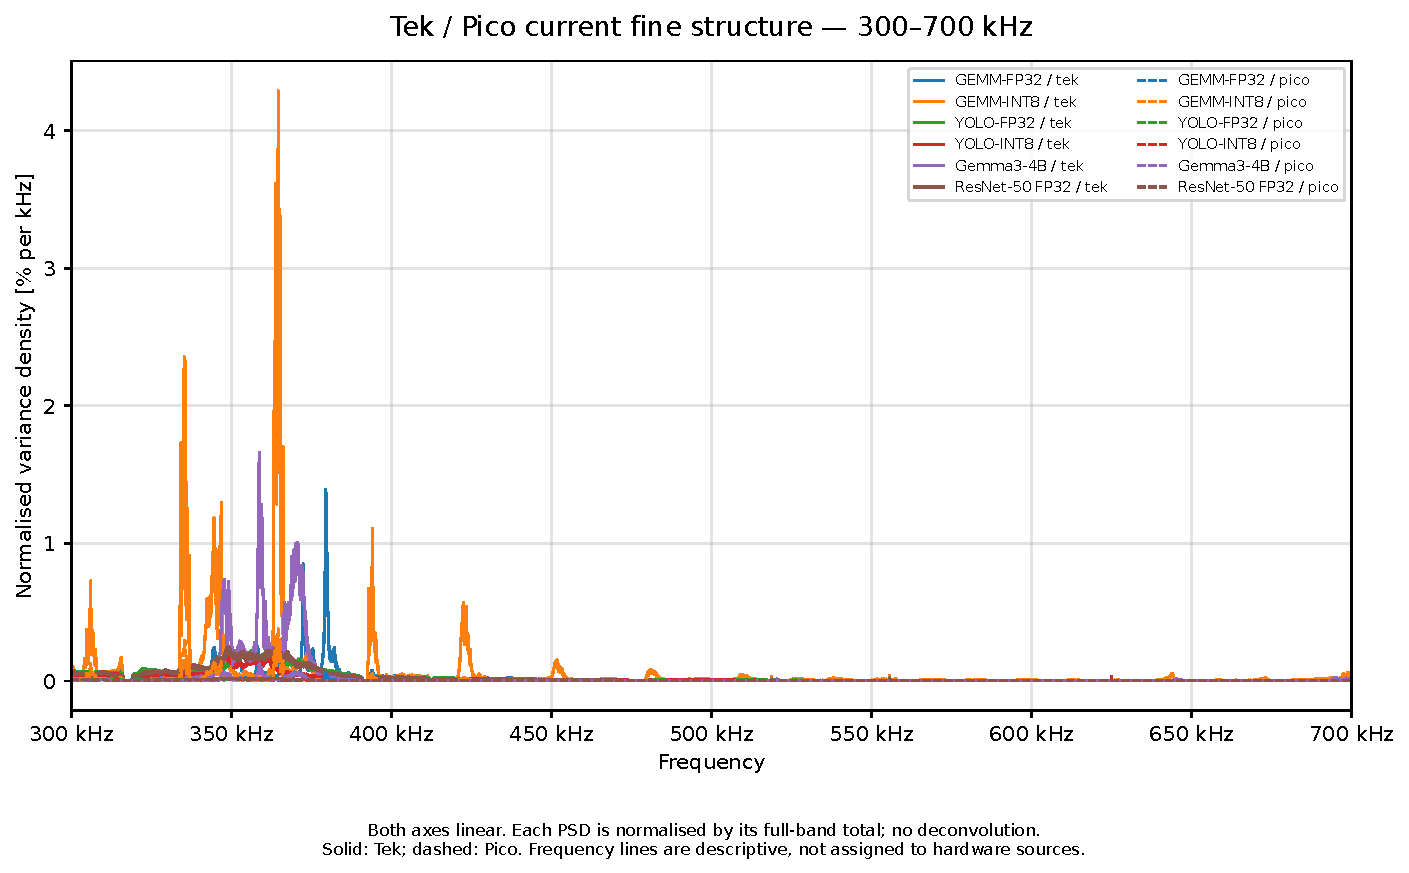
\includegraphics[width=\linewidth]{pico_vs_tek_psd/figures/fine_structure/tek_vs_pico_fine_300000_700000hz.pdf}
\caption{Both axes linear. Each PSD is normalised by its full-band total; no deconvolution.
Solid: Tek; dashed: Pico. Frequency lines are descriptive, not assigned to hardware sources.}
\label{fig:journal-pico-vs-tek-psd-figures-fine-structure-tek-vs-pico-fine-300000-700000hz}
\end{figure}

\begin{figure}[tbp]
\centering
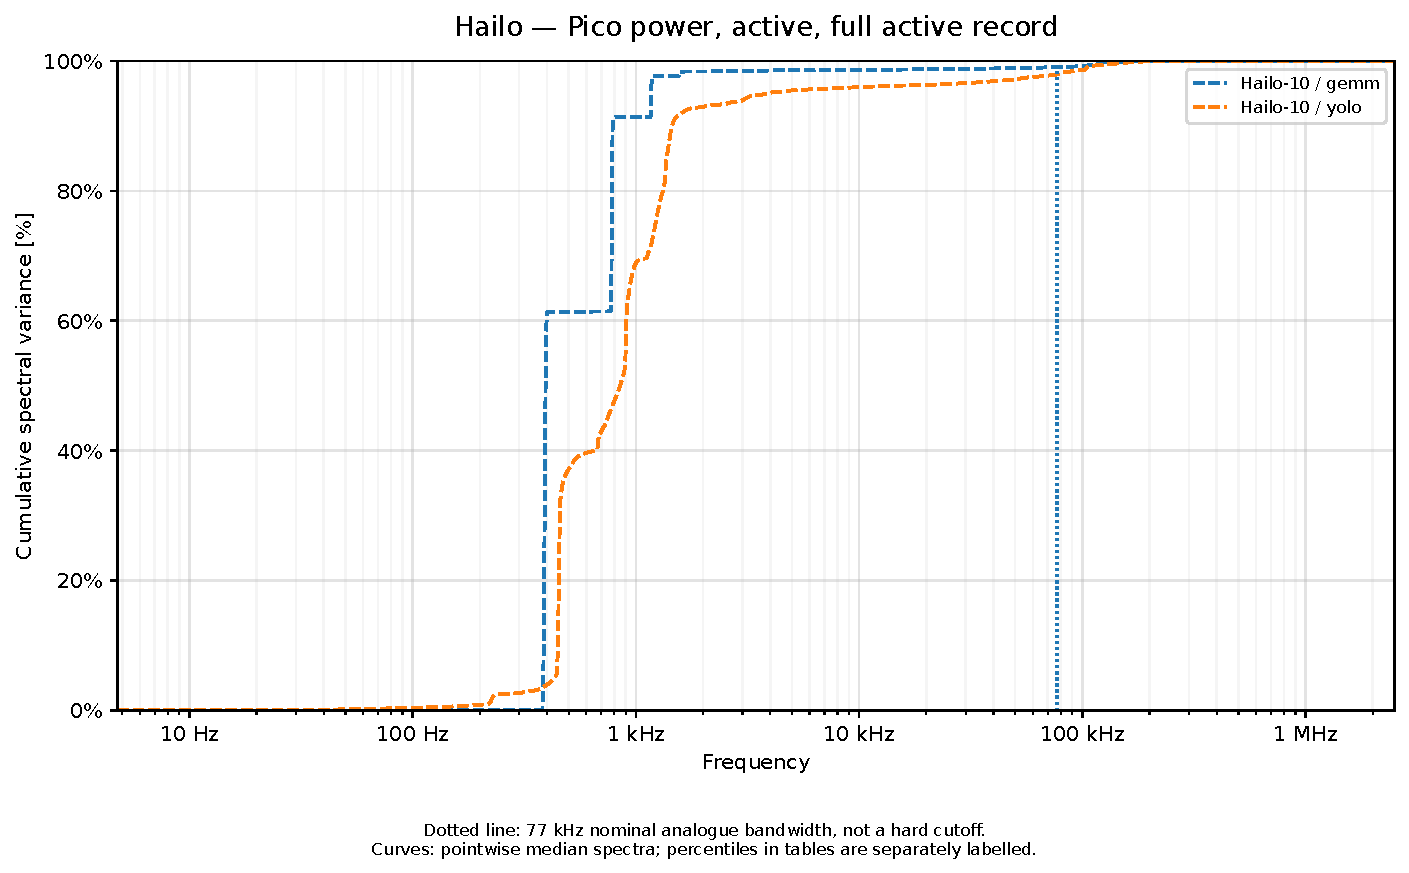
\includegraphics[width=\linewidth]{cross_platform_psd/figures/hailo_power_active_cumulative.pdf}
\caption{Dotted line: 77 kHz nominal analogue bandwidth, not a hard cutoff.
Curves: pointwise median spectra; percentiles in tables are separately labelled.}
\label{fig:journal-cross-platform-psd-figures-hailo-power-active-cumulative}
\end{figure}

\begin{figure}[tbp]
\centering
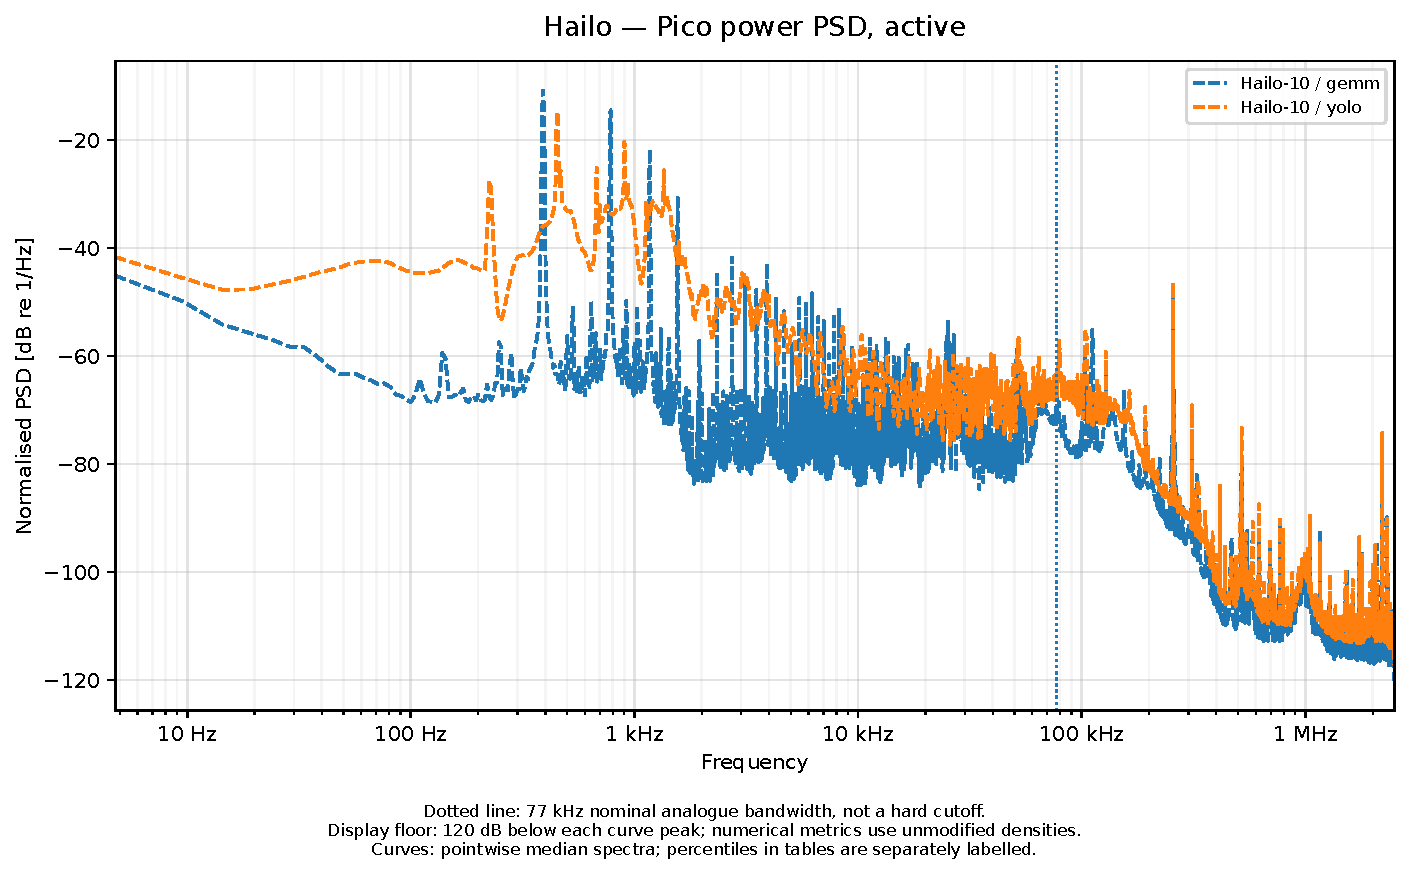
\includegraphics[width=\linewidth]{cross_platform_psd/figures/hailo_power_active_psd.pdf}
\caption{Dotted line: 77 kHz nominal analogue bandwidth, not a hard cutoff.
Display floor: 120 dB below each curve peak; numerical metrics use unmodified densities.
Curves: pointwise median spectra; percentiles in tables are separately labelled.}
\label{fig:journal-cross-platform-psd-figures-hailo-power-active-psd}
\end{figure}

\begin{figure}[tbp]
\centering
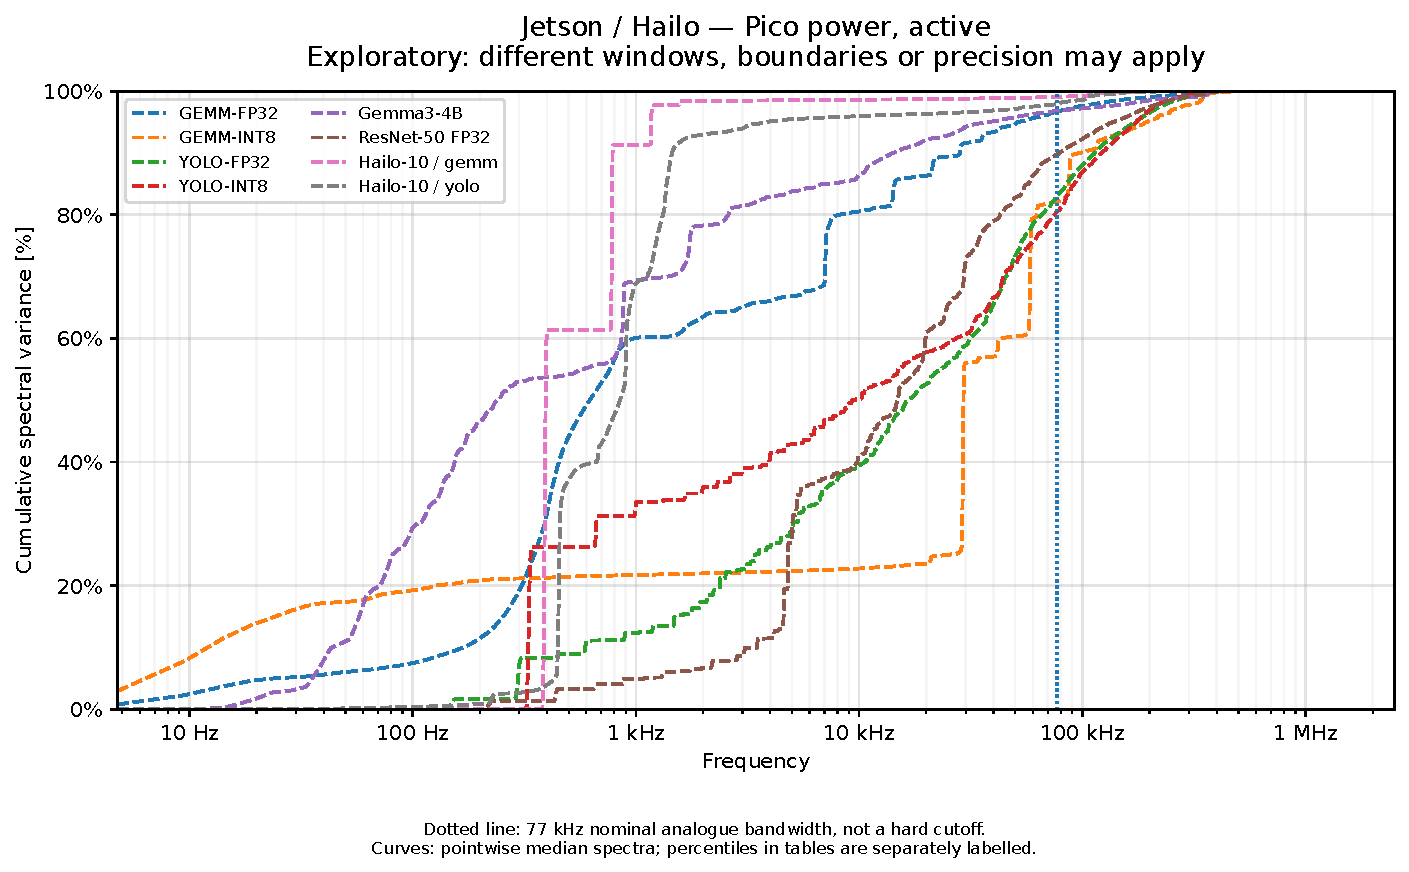
\includegraphics[width=\linewidth]{cross_platform_psd/figures/jetson_vs_hailo_pico_power_active_cumulative_exploratory.pdf}
\caption{Dotted line: 77 kHz nominal analogue bandwidth, not a hard cutoff.
Curves: pointwise median spectra; percentiles in tables are separately labelled.}
\label{fig:journal-cross-platform-psd-figures-jetson-vs-hailo-pico-power-active-cumulative-exploratory}
\end{figure}

\begin{figure}[tbp]
\centering
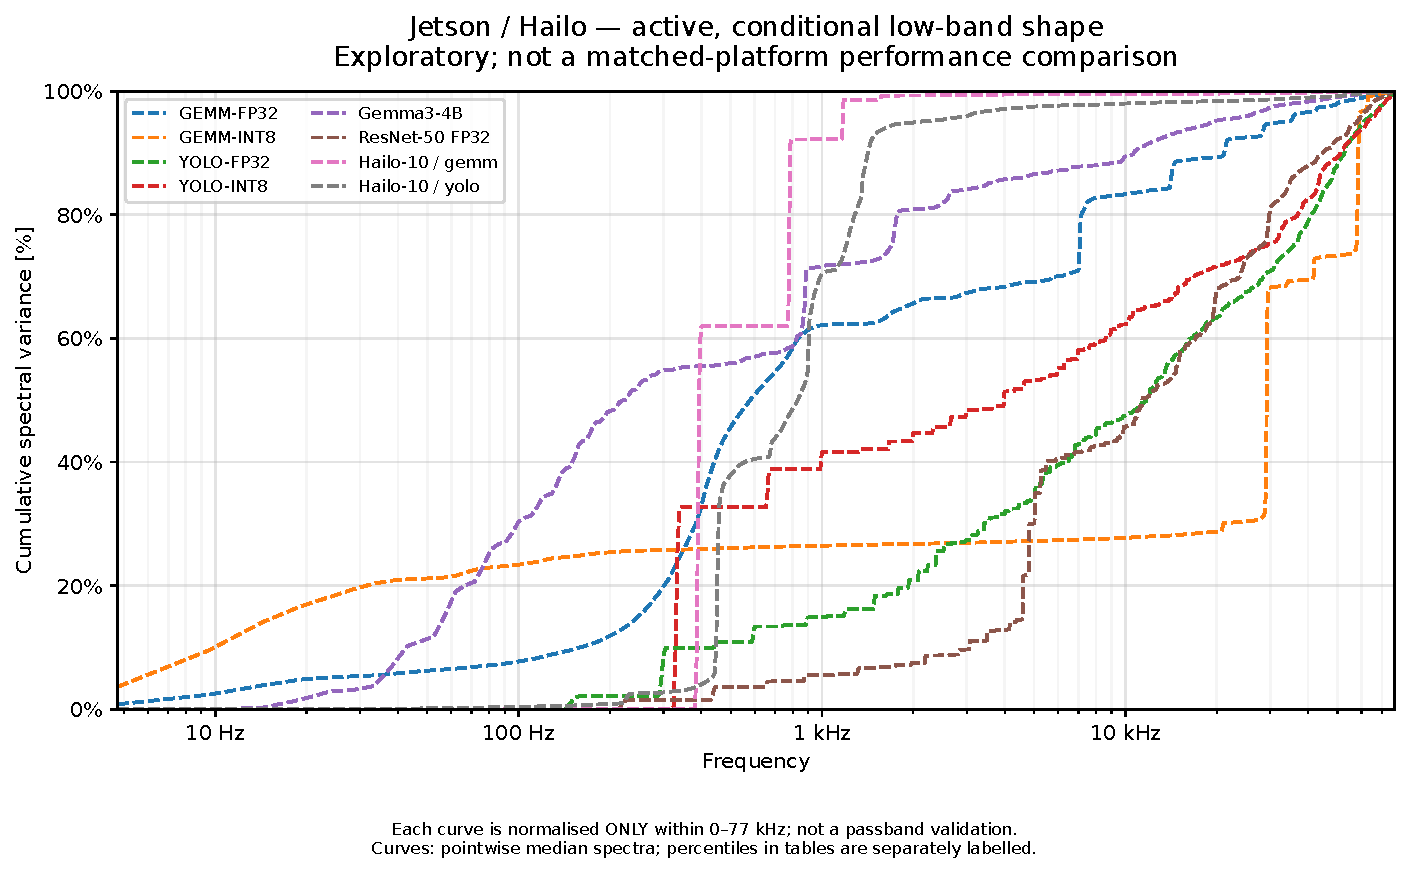
\includegraphics[width=\linewidth]{cross_platform_psd/figures/jetson_vs_hailo_pico_power_active_conditional_0_77khz.pdf}
\caption{Each curve is normalised ONLY within 0--77 kHz; not a passband validation.
Curves: pointwise median spectra; percentiles in tables are separately labelled.}
\label{fig:journal-cross-platform-psd-figures-jetson-vs-hailo-pico-power-active-conditional-0-77khz}
\end{figure}

\begin{figure}[tbp]
\centering
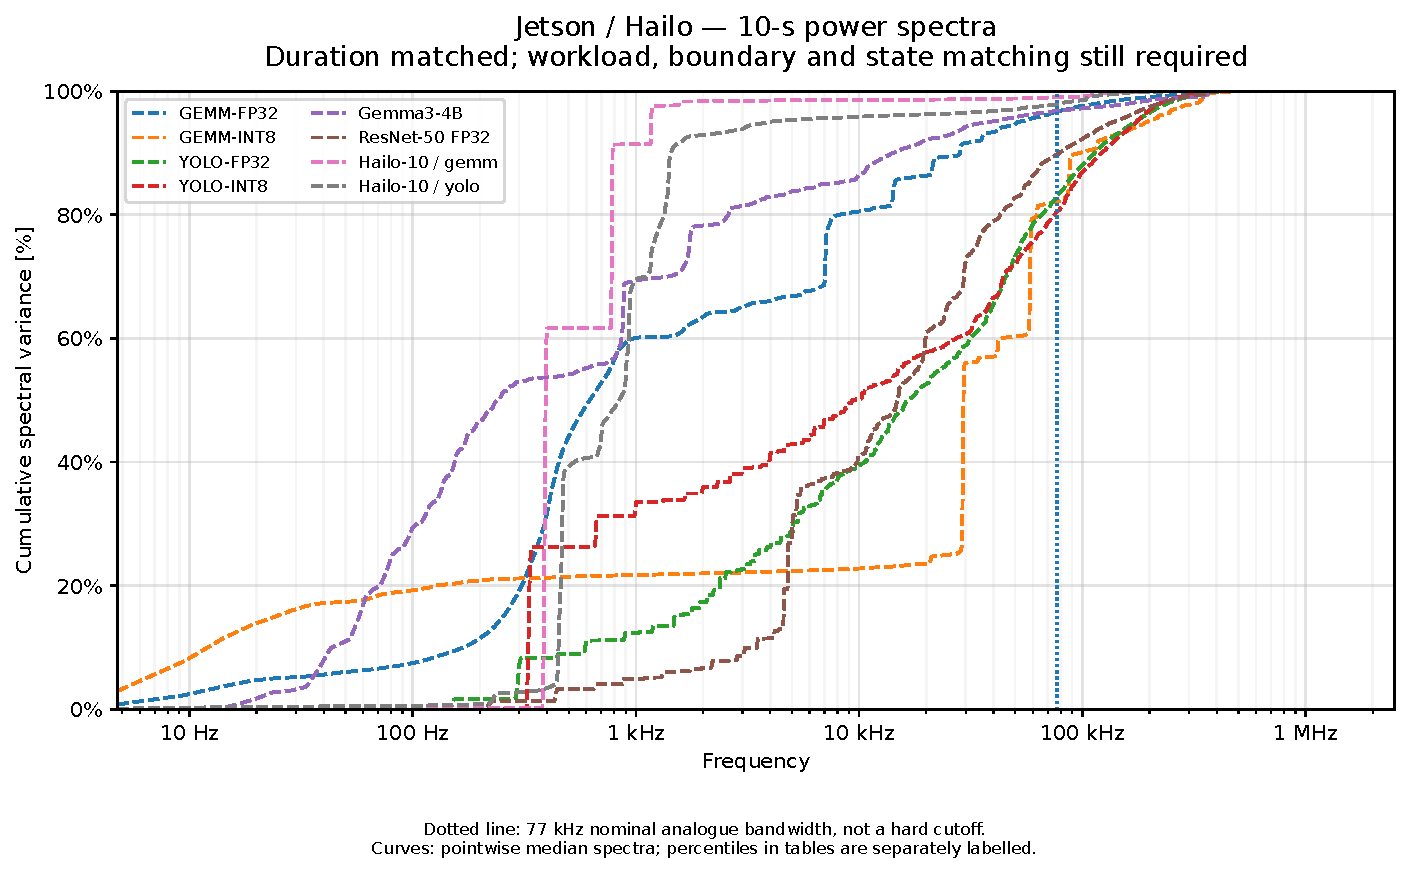
\includegraphics[width=\linewidth]{cross_platform_psd/figures/jetson_vs_hailo_pico_power_active_matched_duration.pdf}
\caption{Dotted line: 77 kHz nominal analogue bandwidth, not a hard cutoff.
Curves: pointwise median spectra; percentiles in tables are separately labelled.}
\label{fig:journal-cross-platform-psd-figures-jetson-vs-hailo-pico-power-active-matched-duration}
\end{figure}

\begin{figure}[tbp]
\centering
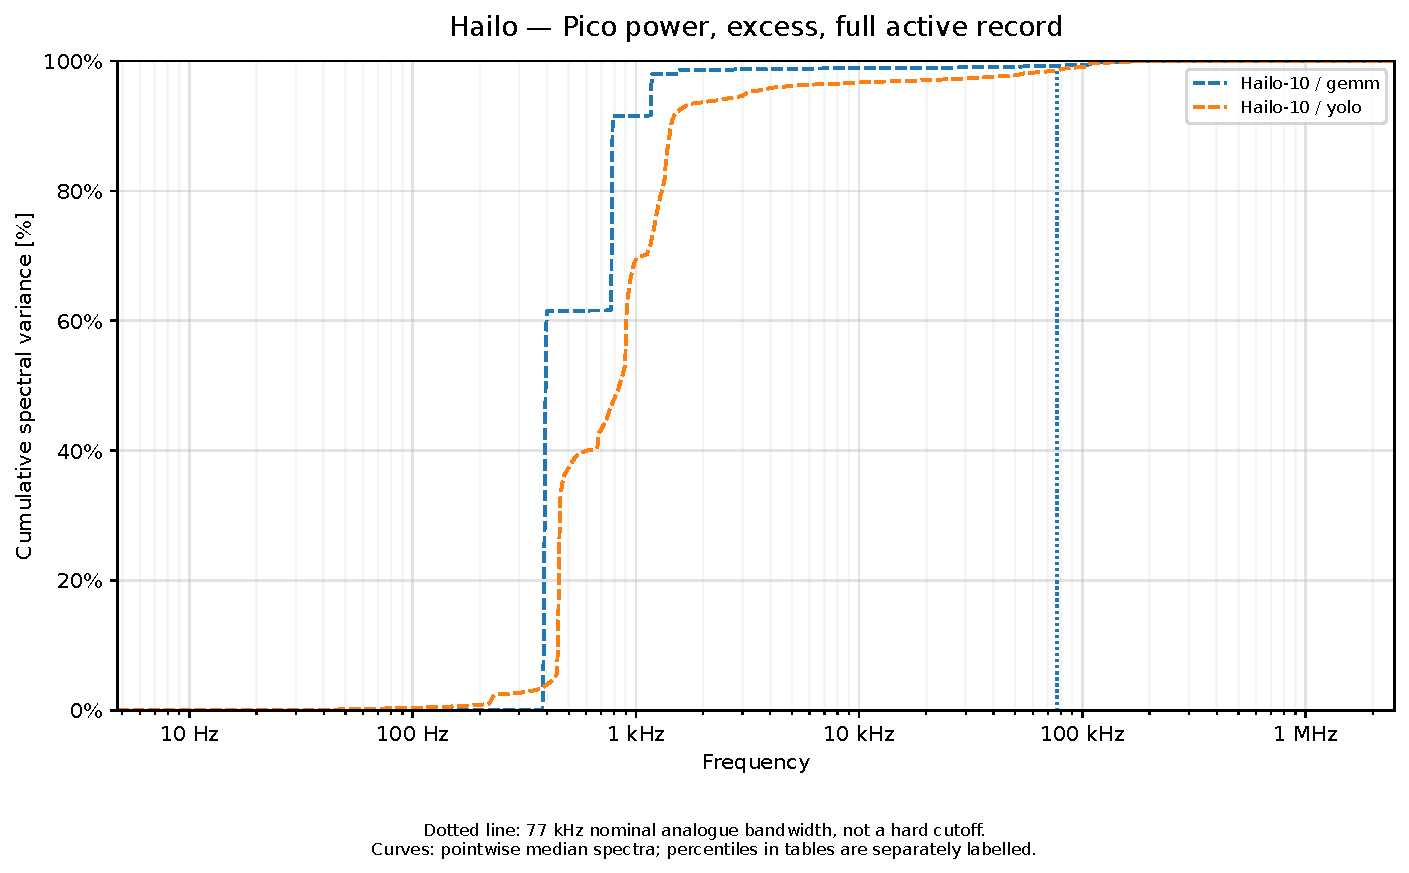
\includegraphics[width=\linewidth]{cross_platform_psd/figures/hailo_power_excess_cumulative.pdf}
\caption{Dotted line: 77 kHz nominal analogue bandwidth, not a hard cutoff.
Curves: pointwise median spectra; percentiles in tables are separately labelled.}
\label{fig:journal-cross-platform-psd-figures-hailo-power-excess-cumulative}
\end{figure}

\begin{figure}[tbp]
\centering
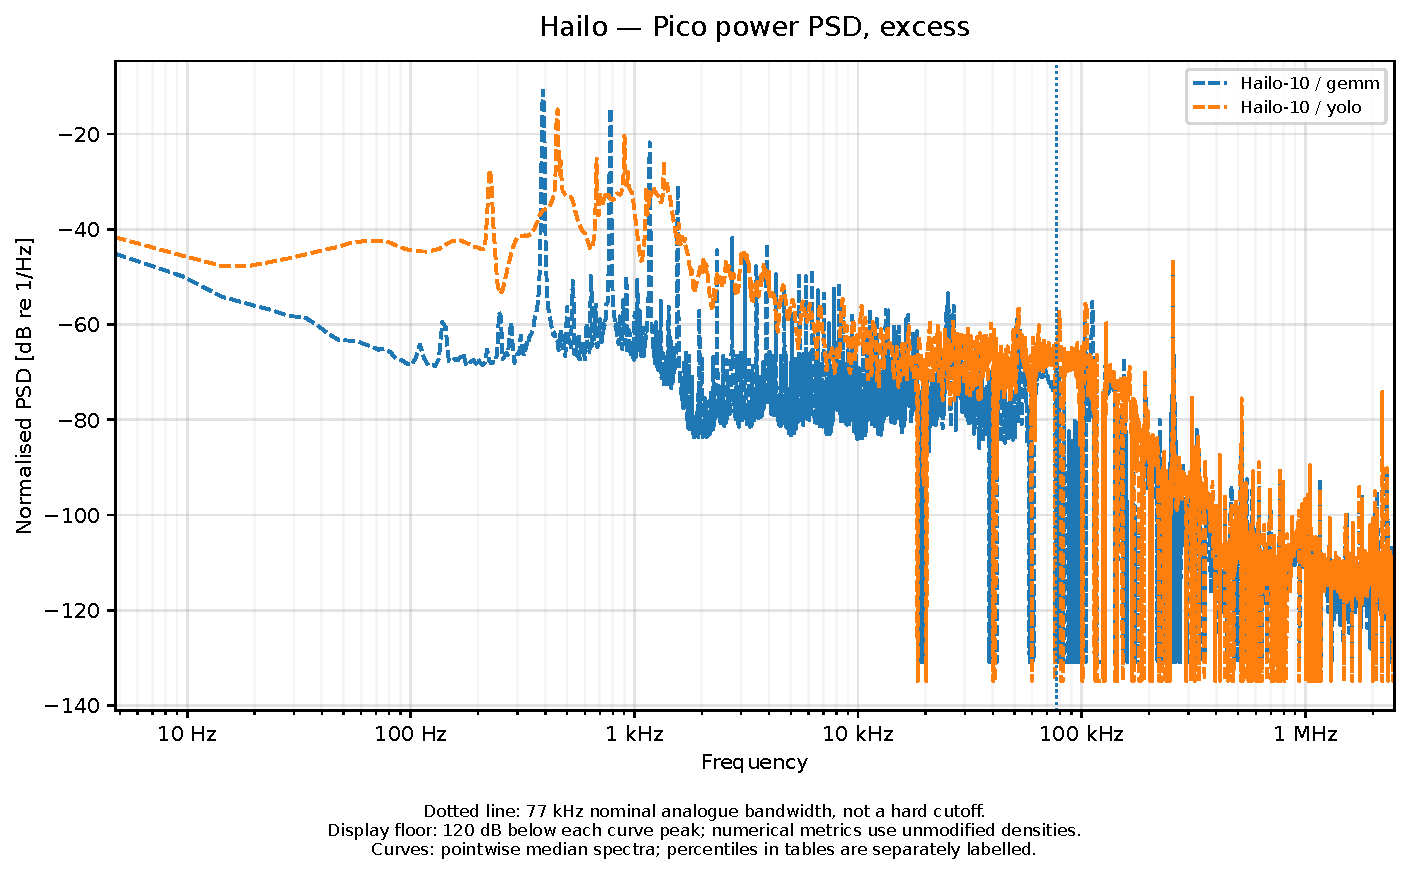
\includegraphics[width=\linewidth]{cross_platform_psd/figures/hailo_power_excess_psd.pdf}
\caption{Dotted line: 77 kHz nominal analogue bandwidth, not a hard cutoff.
Display floor: 120 dB below each curve peak; numerical metrics use unmodified densities.
Curves: pointwise median spectra; percentiles in tables are separately labelled.}
\label{fig:journal-cross-platform-psd-figures-hailo-power-excess-psd}
\end{figure}

\begin{figure}[tbp]
\centering
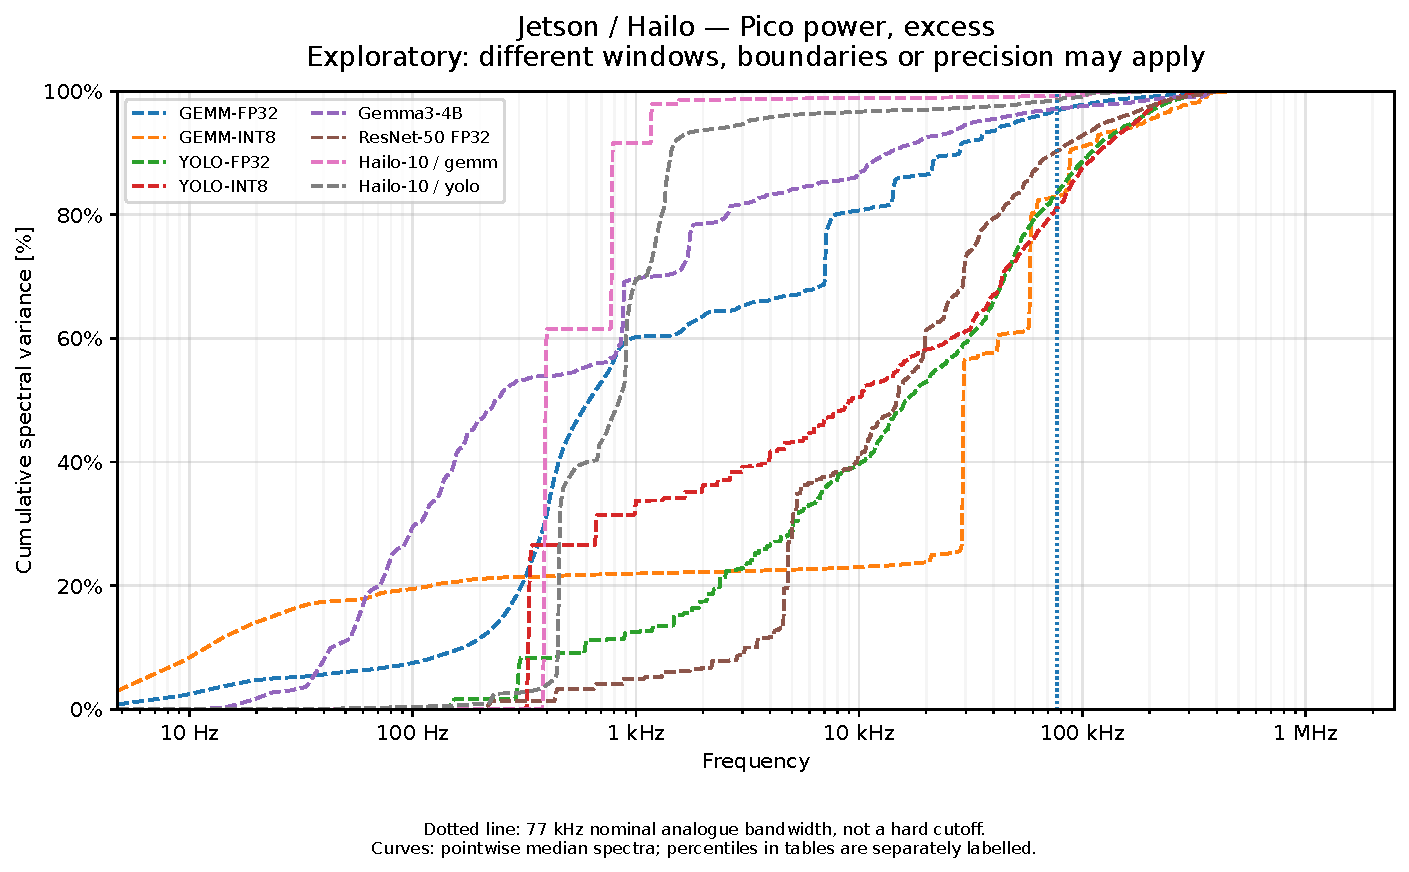
\includegraphics[width=\linewidth]{cross_platform_psd/figures/jetson_vs_hailo_pico_power_excess_cumulative_exploratory.pdf}
\caption{Dotted line: 77 kHz nominal analogue bandwidth, not a hard cutoff.
Curves: pointwise median spectra; percentiles in tables are separately labelled.}
\label{fig:journal-cross-platform-psd-figures-jetson-vs-hailo-pico-power-excess-cumulative-exploratory}
\end{figure}

\begin{figure}[tbp]
\centering
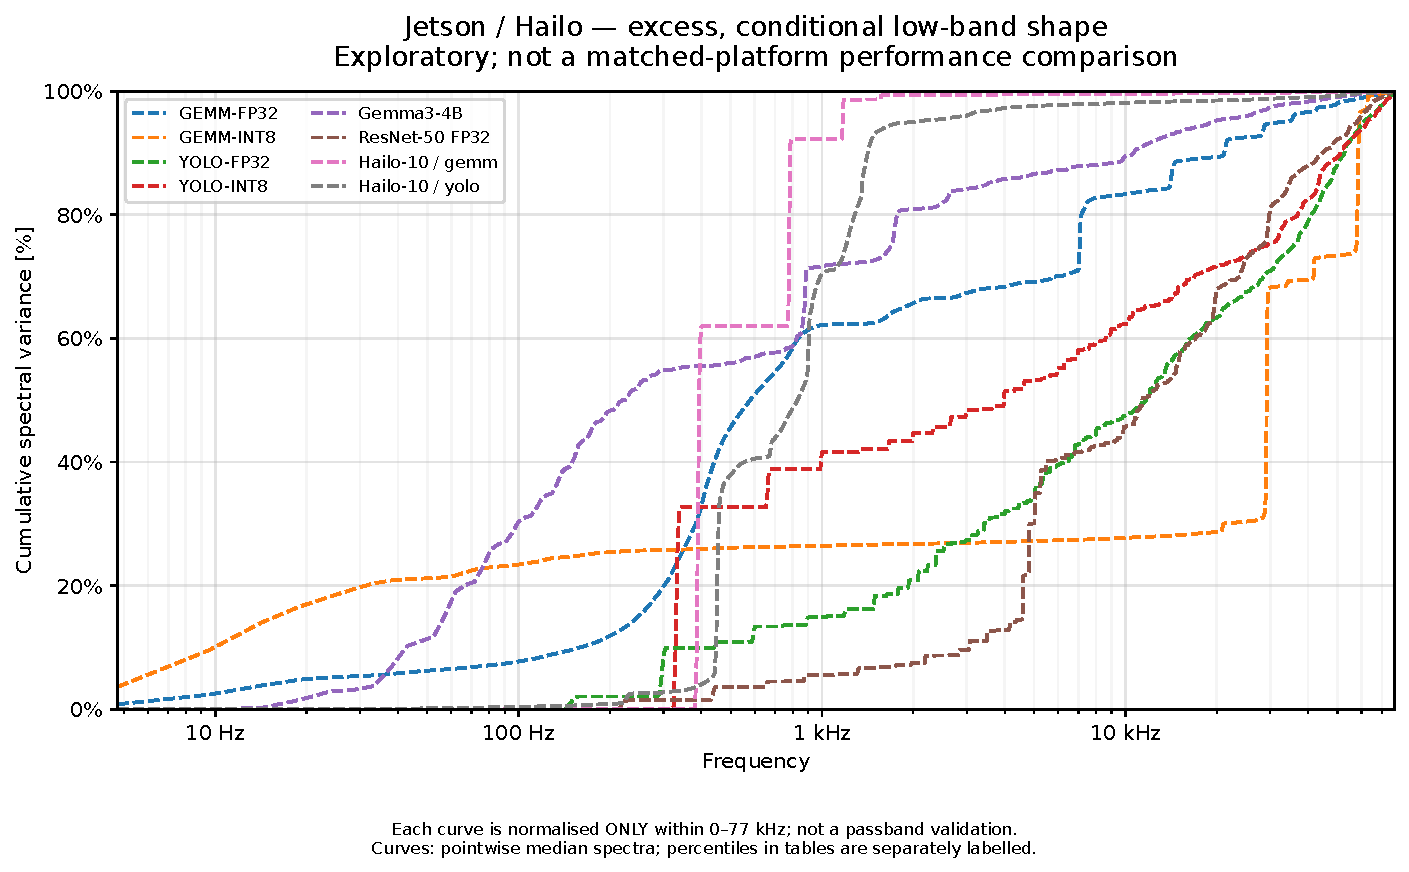
\includegraphics[width=\linewidth]{cross_platform_psd/figures/jetson_vs_hailo_pico_power_excess_conditional_0_77khz.pdf}
\caption{Each curve is normalised ONLY within 0--77 kHz; not a passband validation.
Curves: pointwise median spectra; percentiles in tables are separately labelled.}
\label{fig:journal-cross-platform-psd-figures-jetson-vs-hailo-pico-power-excess-conditional-0-77khz}
\end{figure}

\begin{figure}[tbp]
\centering
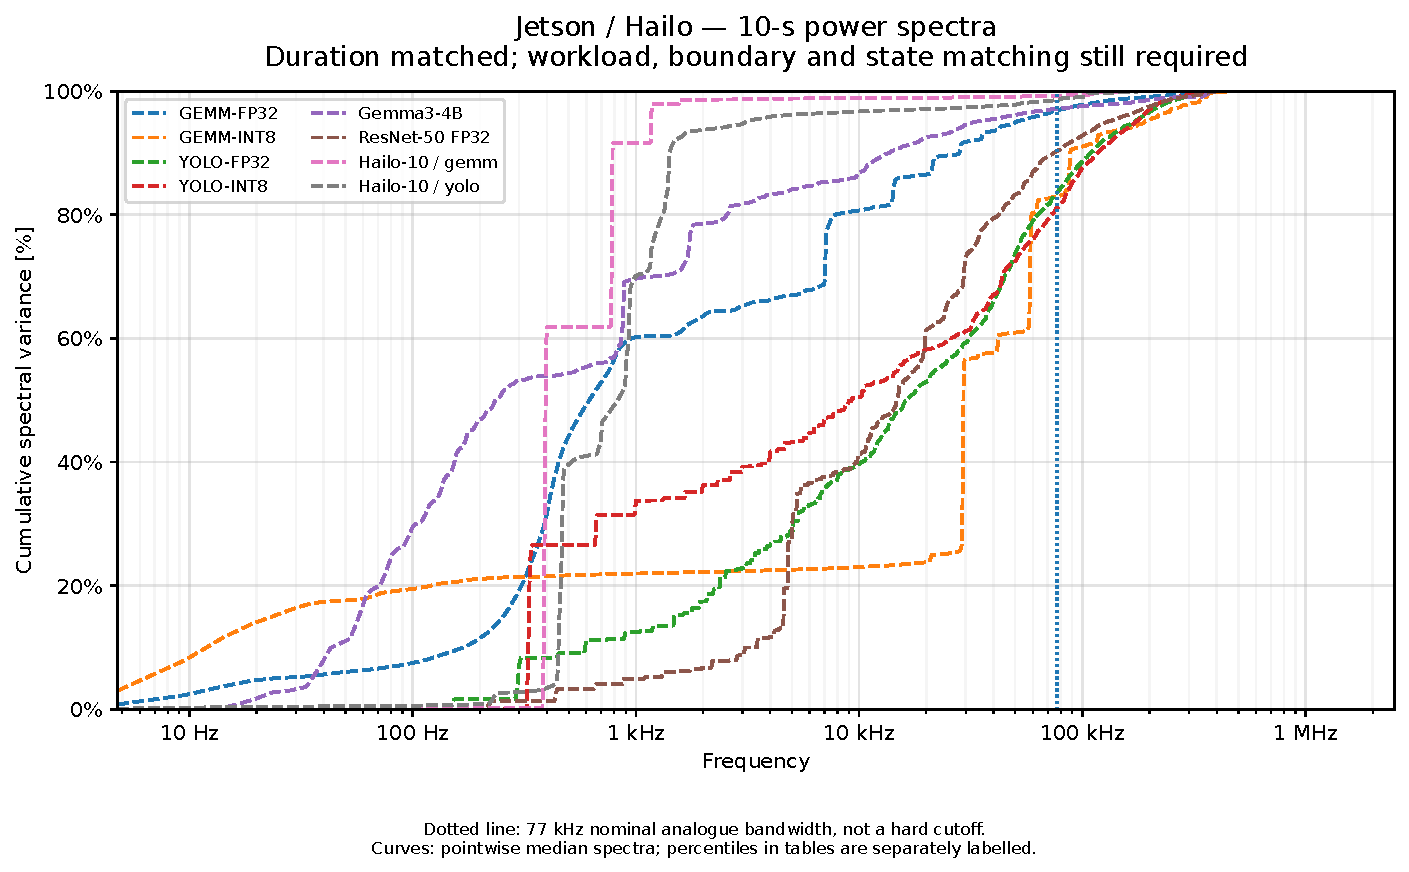
\includegraphics[width=\linewidth]{cross_platform_psd/figures/jetson_vs_hailo_pico_power_excess_matched_duration.pdf}
\caption{Dotted line: 77 kHz nominal analogue bandwidth, not a hard cutoff.
Curves: pointwise median spectra; percentiles in tables are separately labelled.}
\label{fig:journal-cross-platform-psd-figures-jetson-vs-hailo-pico-power-excess-matched-duration}
\end{figure}

\begin{figure}[tbp]
\centering
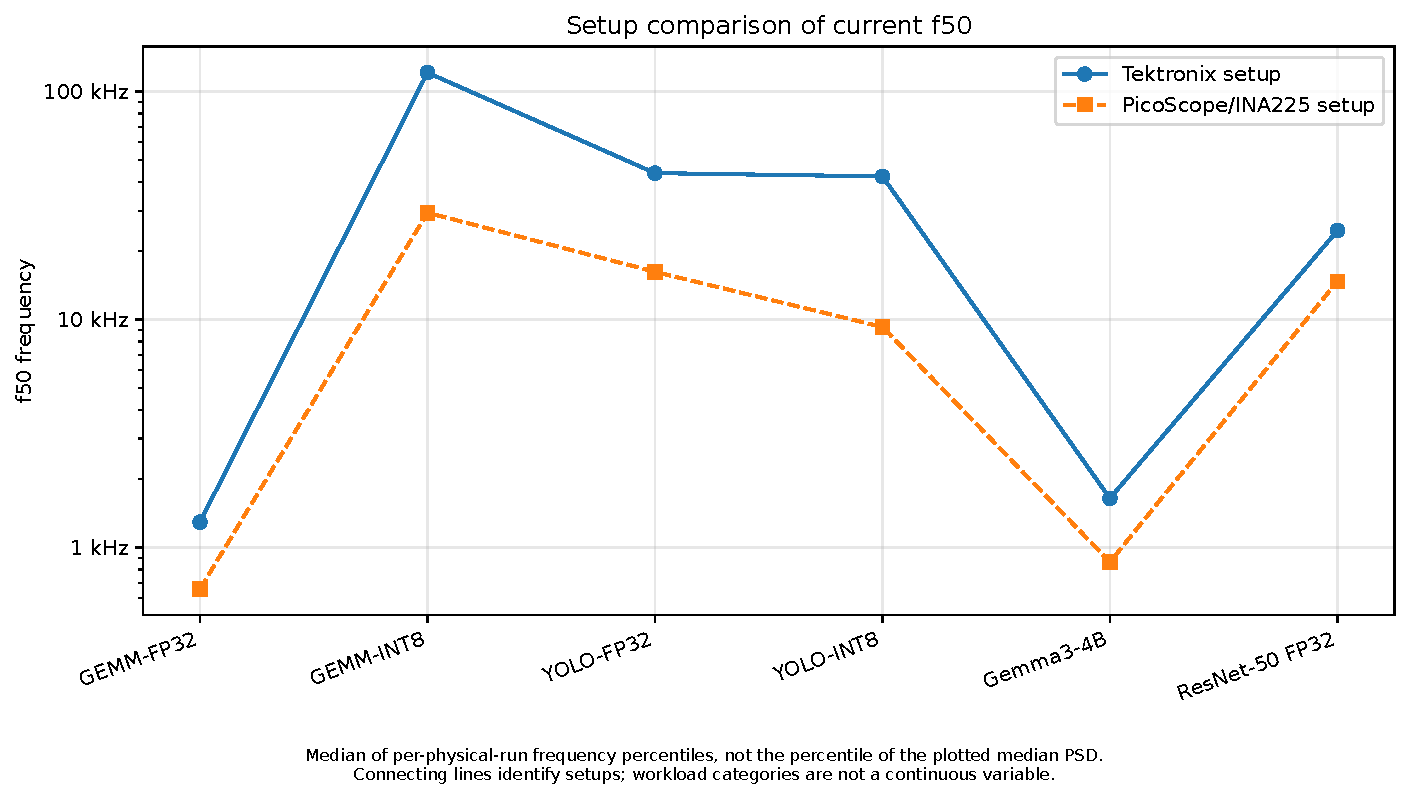
\includegraphics[width=\linewidth]{pico_vs_tek_psd/figures/tek_vs_pico_current_f50.pdf}
\caption{Median of per-physical-run frequency percentiles, not the percentile of the plotted median PSD.
Connecting lines identify setups; workload categories are not a continuous variable.}
\label{fig:journal-pico-vs-tek-psd-figures-tek-vs-pico-current-f50}
\end{figure}

\begin{figure}[tbp]
\centering
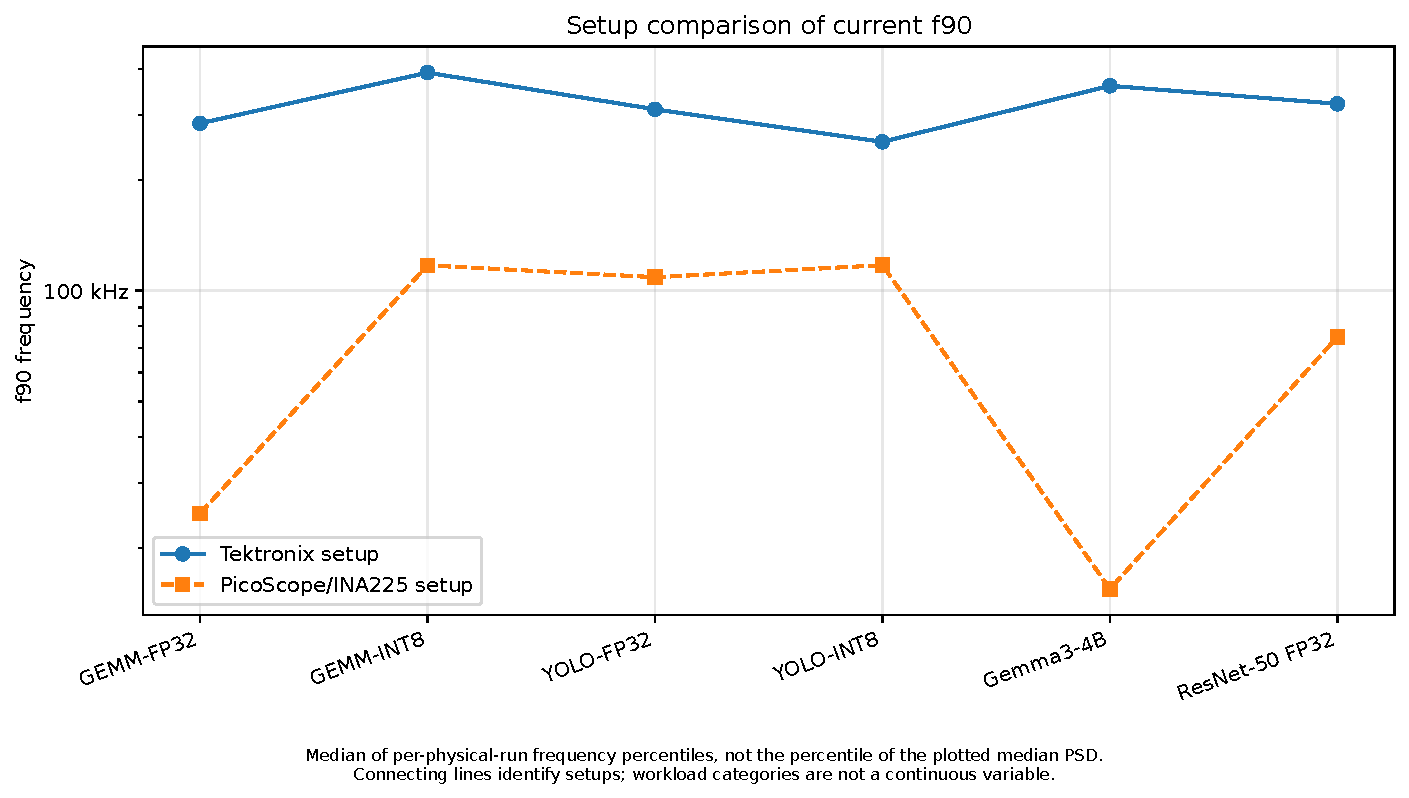
\includegraphics[width=\linewidth]{pico_vs_tek_psd/figures/tek_vs_pico_current_f90.pdf}
\caption{Median of per-physical-run frequency percentiles, not the percentile of the plotted median PSD.
Connecting lines identify setups; workload categories are not a continuous variable.}
\label{fig:journal-pico-vs-tek-psd-figures-tek-vs-pico-current-f90}
\end{figure}

\begin{figure}[tbp]
\centering
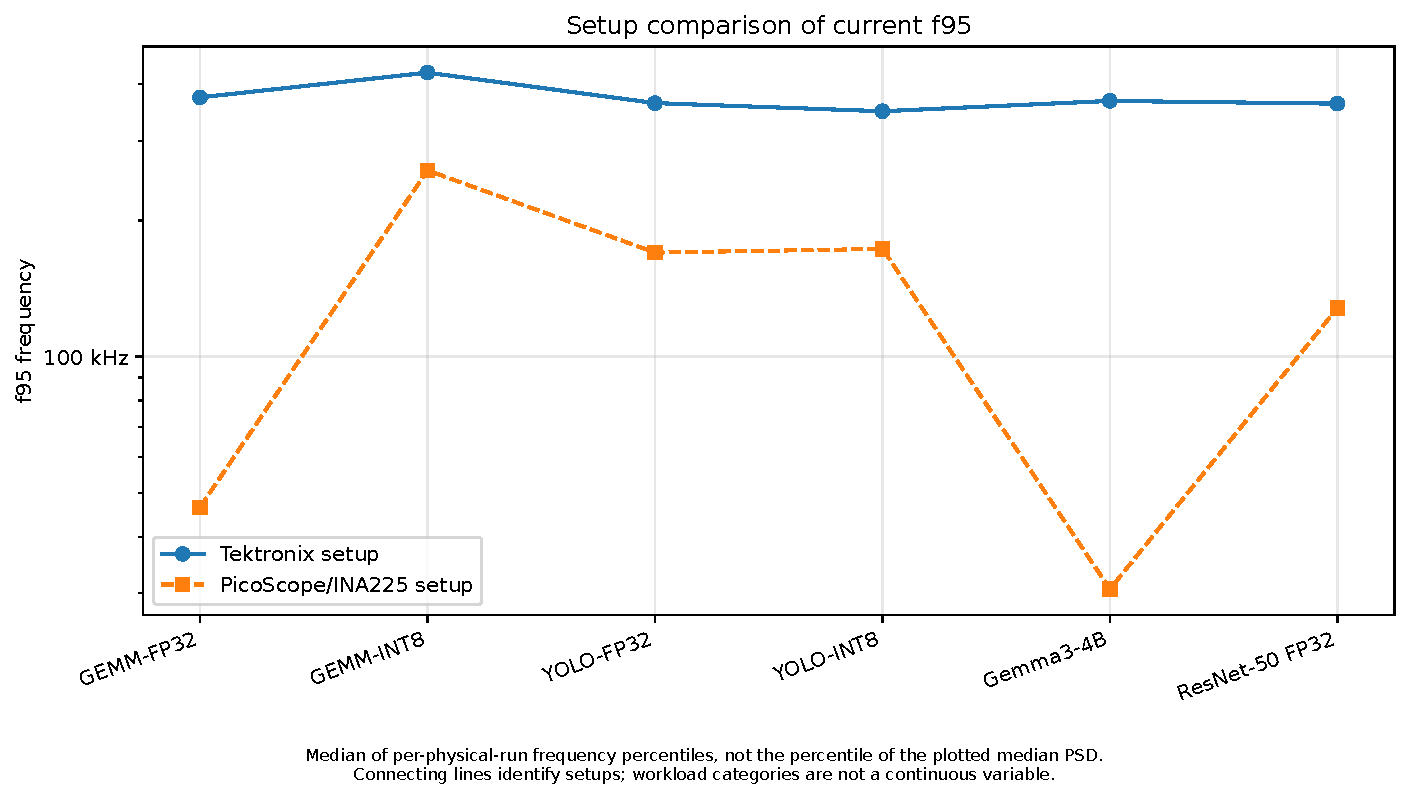
\includegraphics[width=\linewidth]{pico_vs_tek_psd/figures/tek_vs_pico_current_f95.pdf}
\caption{Median of per-physical-run frequency percentiles, not the percentile of the plotted median PSD.
Connecting lines identify setups; workload categories are not a continuous variable.}
\label{fig:journal-pico-vs-tek-psd-figures-tek-vs-pico-current-f95}
\end{figure}

\begin{figure}[tbp]
\centering
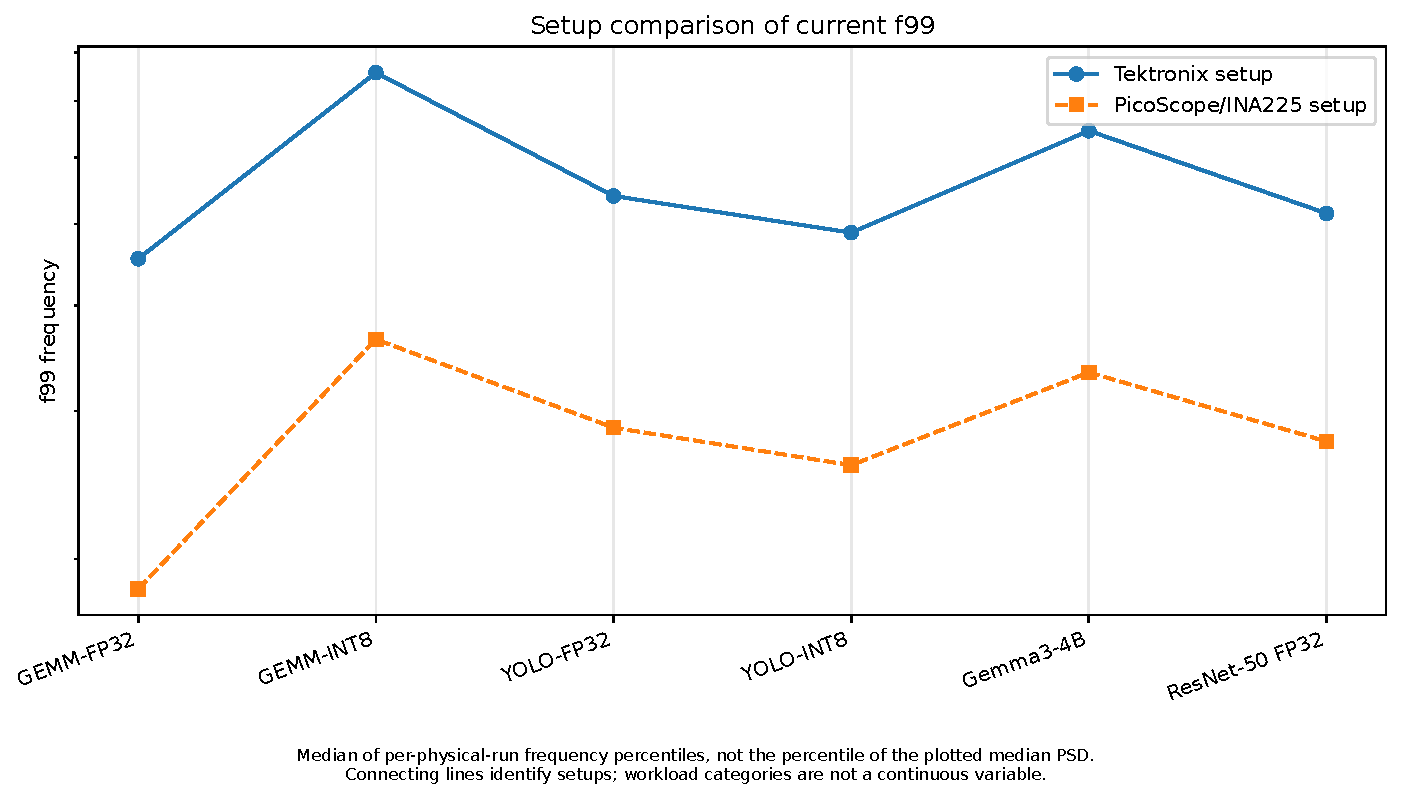
\includegraphics[width=\linewidth]{pico_vs_tek_psd/figures/tek_vs_pico_current_f99.pdf}
\caption{Median of per-physical-run frequency percentiles, not the percentile of the plotted median PSD.
Connecting lines identify setups; workload categories are not a continuous variable.}
\label{fig:journal-pico-vs-tek-psd-figures-tek-vs-pico-current-f99}
\end{figure}

\begin{figure}[tbp]
\centering
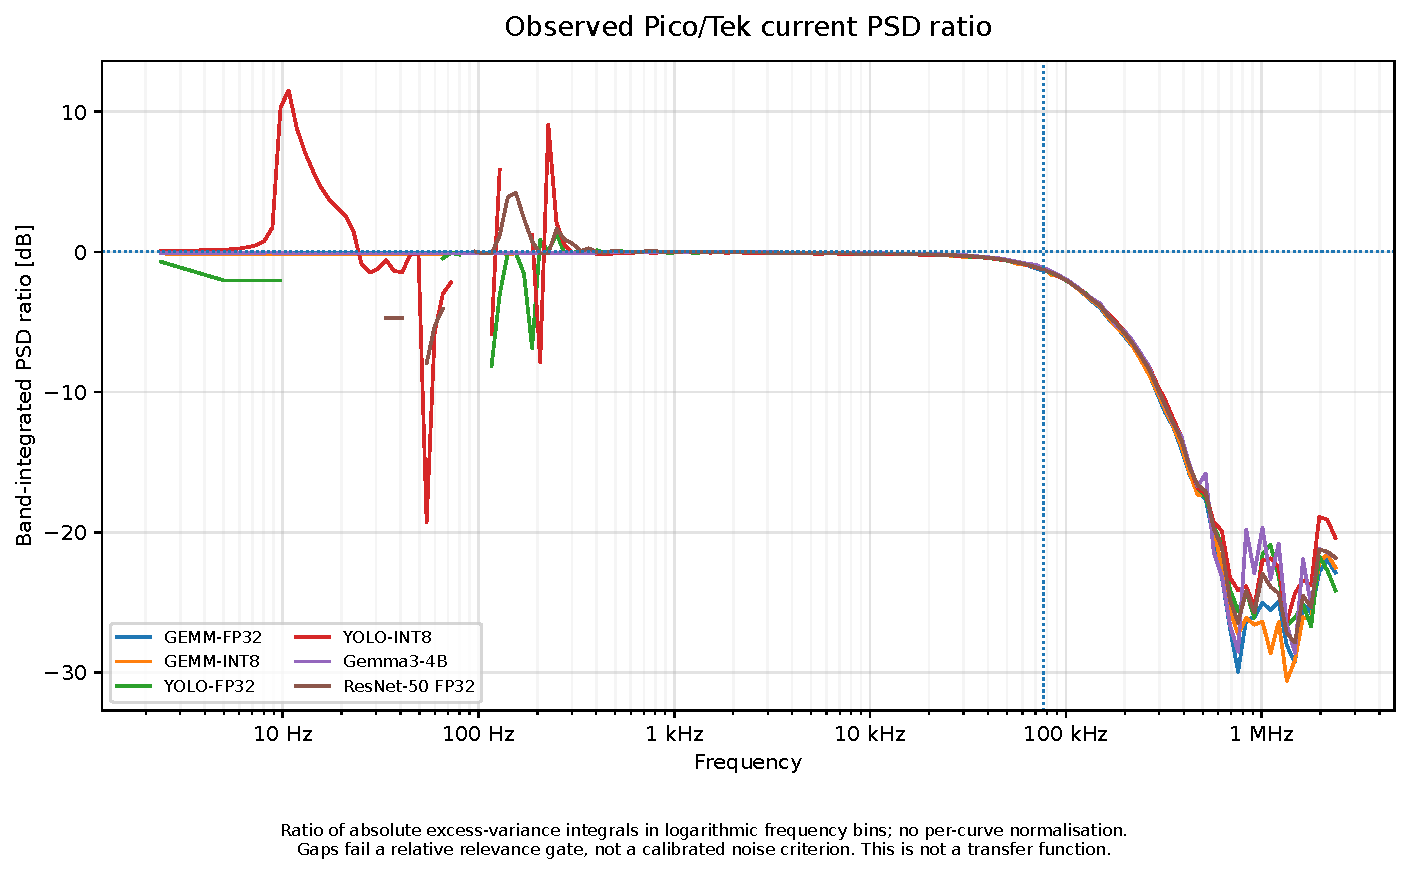
\includegraphics[width=\linewidth]{pico_vs_tek_psd/figures/tek_vs_pico_current_observed_psd_ratio.pdf}
\caption{Ratio of absolute excess-variance integrals in logarithmic frequency bins; no per-curve normalisation.
Gaps fail a relative relevance gate, not a calibrated noise criterion. This is not a transfer function.}
\label{fig:journal-pico-vs-tek-psd-figures-tek-vs-pico-current-observed-psd-ratio}
\end{figure}

\begin{figure}[tbp]
\centering
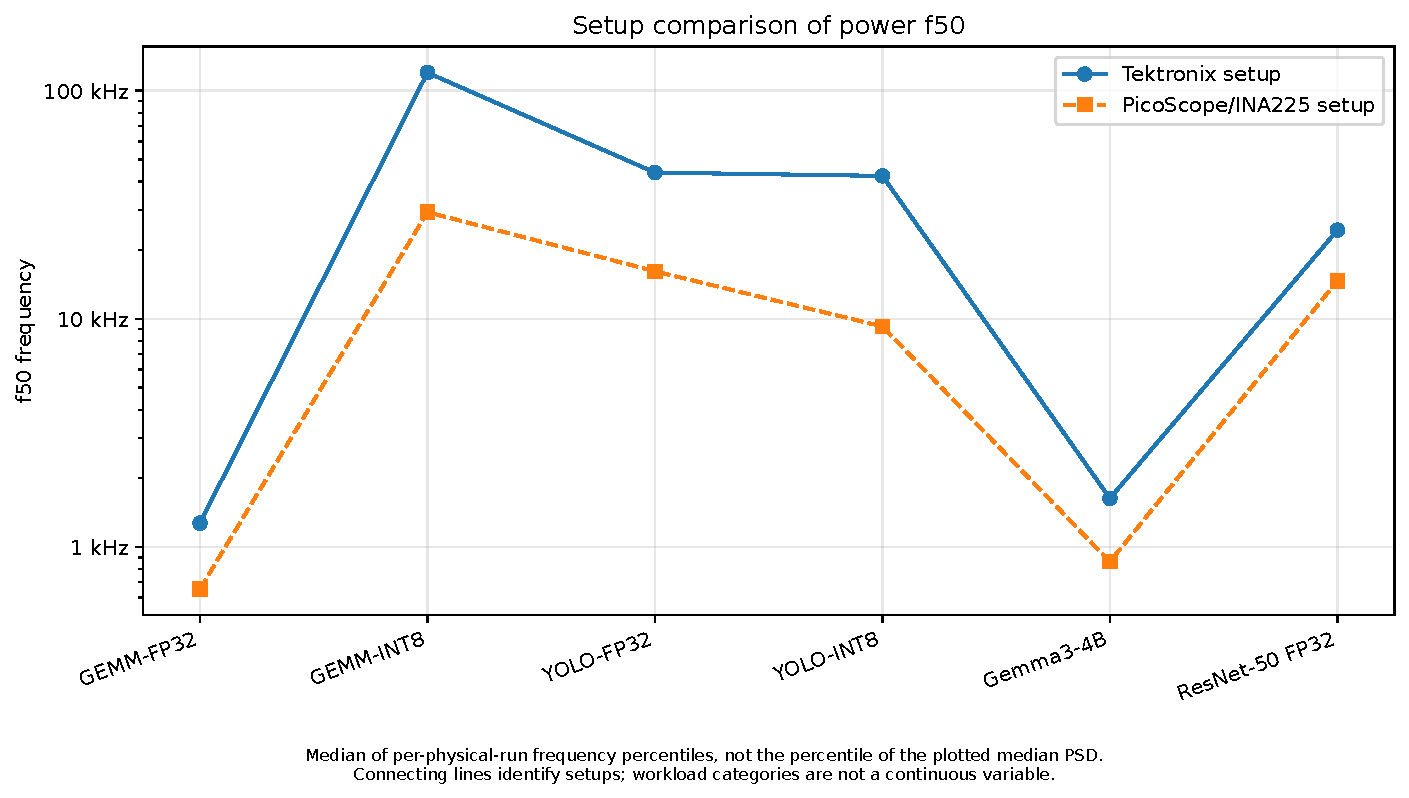
\includegraphics[width=\linewidth]{pico_vs_tek_psd/figures/tek_vs_pico_power_f50.pdf}
\caption{Median of per-physical-run frequency percentiles, not the percentile of the plotted median PSD.
Connecting lines identify setups; workload categories are not a continuous variable.}
\label{fig:journal-pico-vs-tek-psd-figures-tek-vs-pico-power-f50}
\end{figure}

\begin{figure}[tbp]
\centering
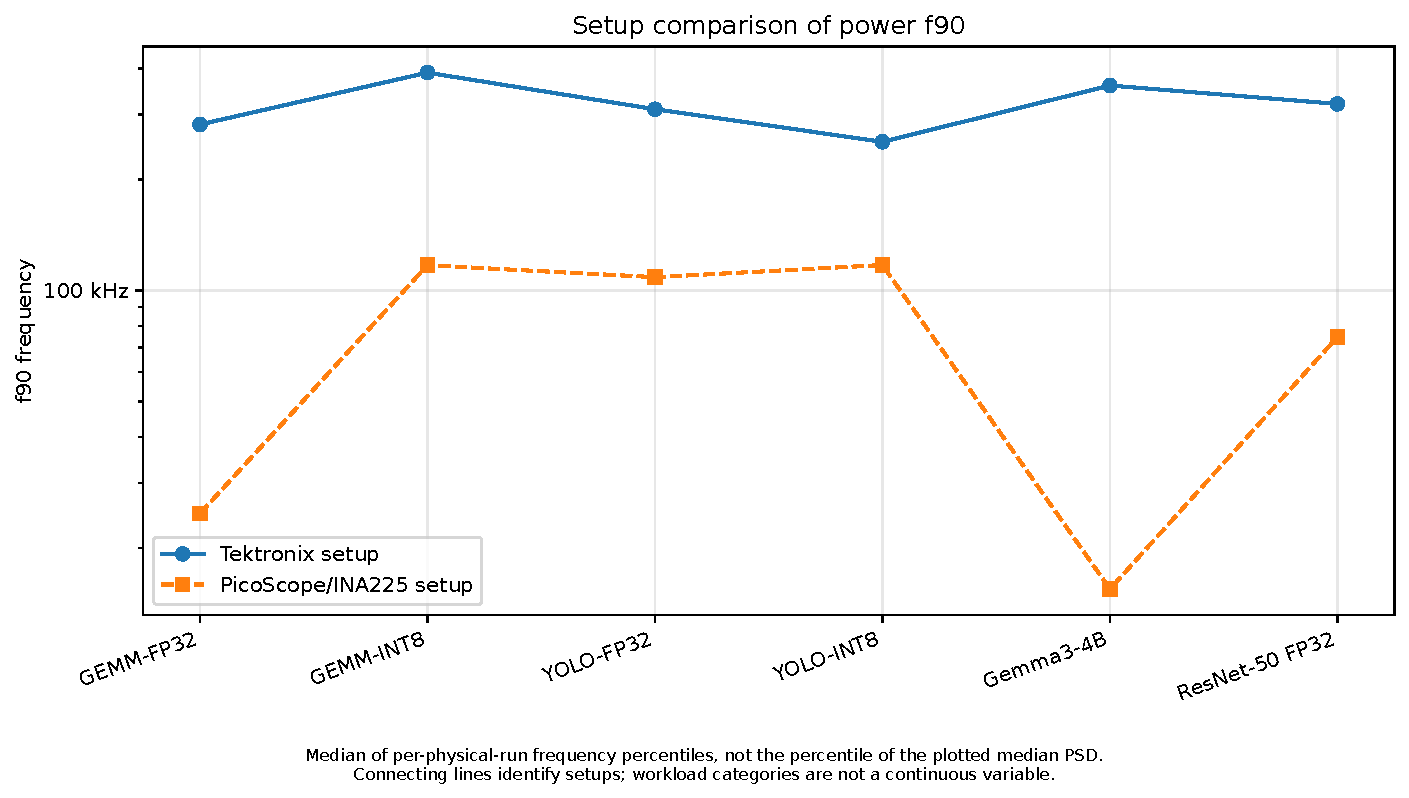
\includegraphics[width=\linewidth]{pico_vs_tek_psd/figures/tek_vs_pico_power_f90.pdf}
\caption{Median of per-physical-run frequency percentiles, not the percentile of the plotted median PSD.
Connecting lines identify setups; workload categories are not a continuous variable.}
\label{fig:journal-pico-vs-tek-psd-figures-tek-vs-pico-power-f90}
\end{figure}

\begin{figure}[tbp]
\centering
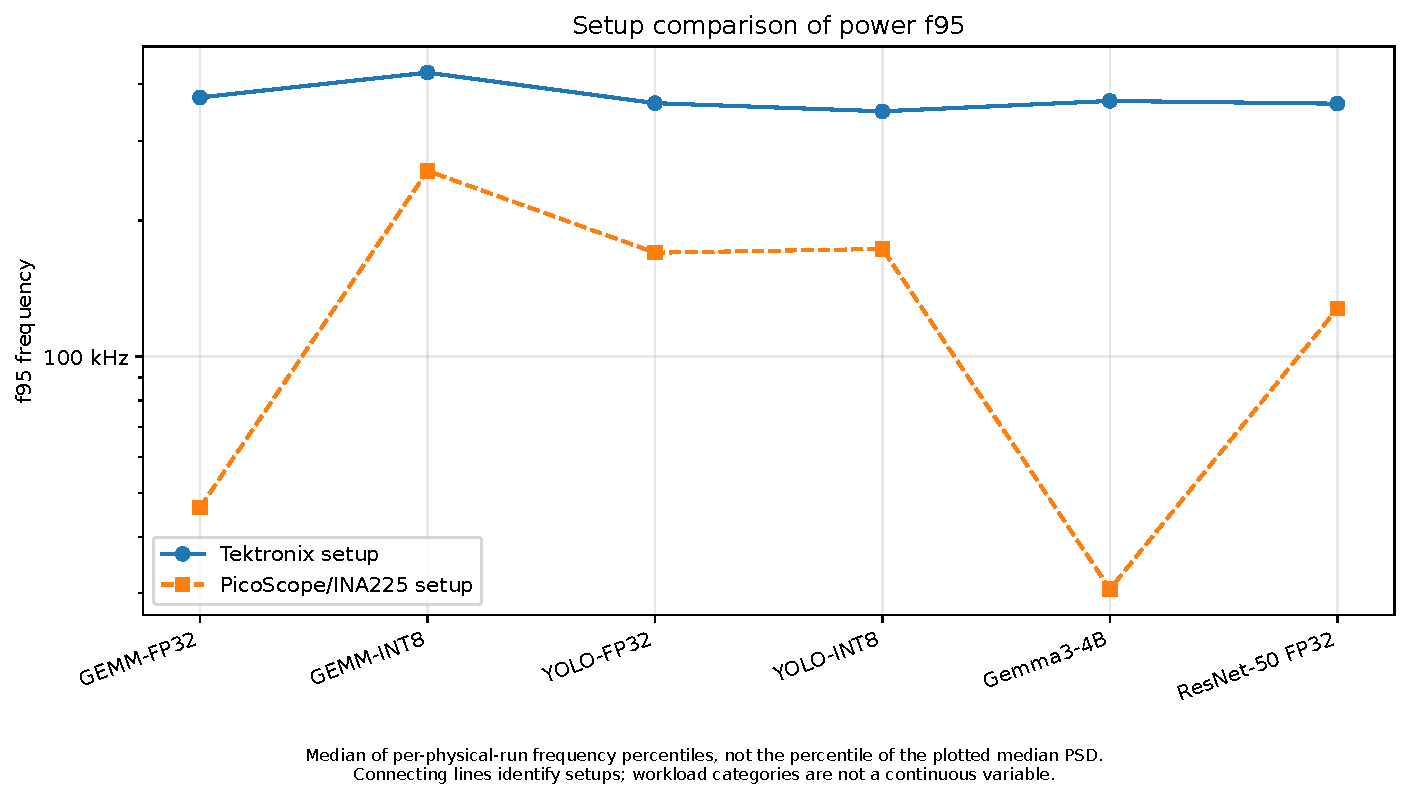
\includegraphics[width=\linewidth]{pico_vs_tek_psd/figures/tek_vs_pico_power_f95.pdf}
\caption{Median of per-physical-run frequency percentiles, not the percentile of the plotted median PSD.
Connecting lines identify setups; workload categories are not a continuous variable.}
\label{fig:journal-pico-vs-tek-psd-figures-tek-vs-pico-power-f95}
\end{figure}

\begin{figure}[tbp]
\centering
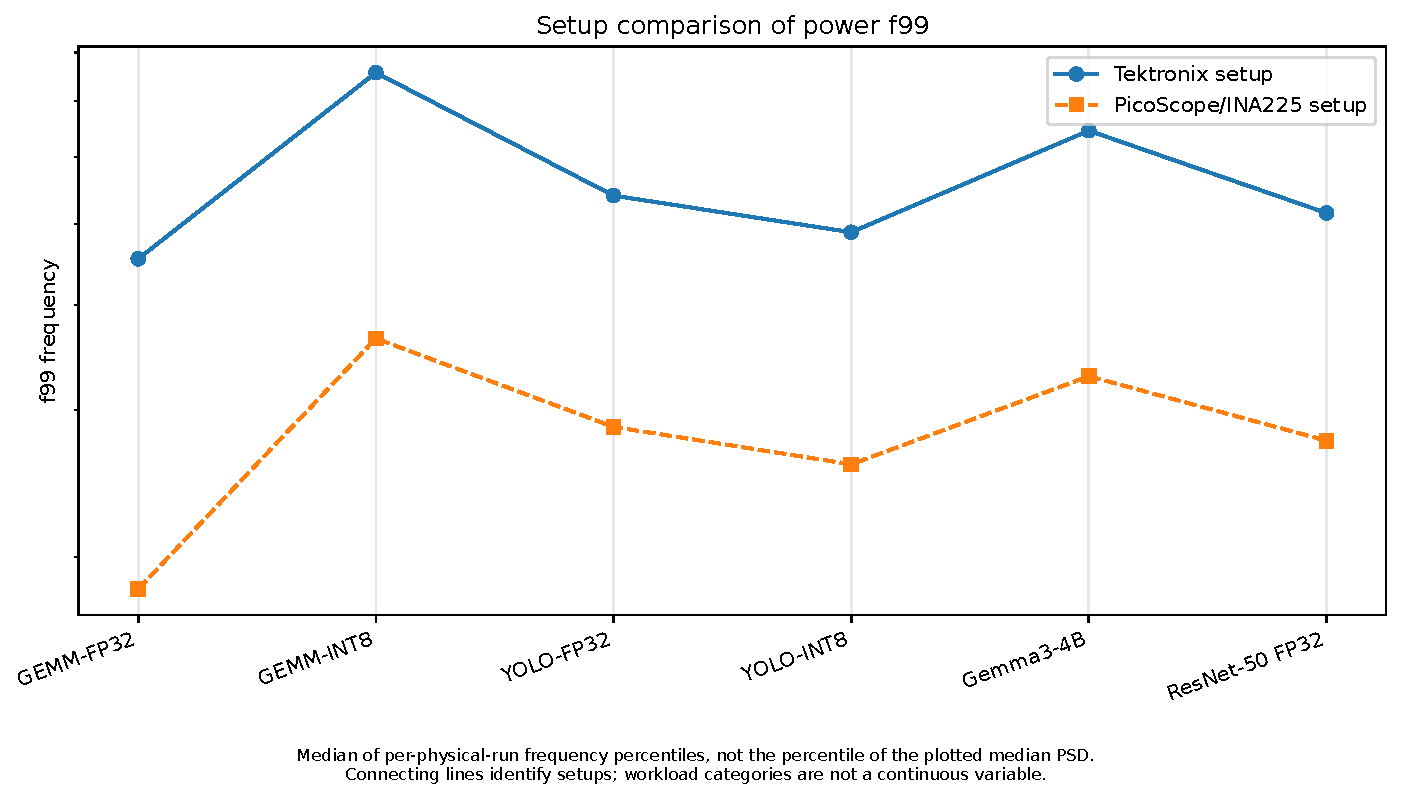
\includegraphics[width=\linewidth]{pico_vs_tek_psd/figures/tek_vs_pico_power_f99.pdf}
\caption{Median of per-physical-run frequency percentiles, not the percentile of the plotted median PSD.
Connecting lines identify setups; workload categories are not a continuous variable.}
\label{fig:journal-pico-vs-tek-psd-figures-tek-vs-pico-power-f99}
\end{figure}

\begin{figure}[tbp]
\centering
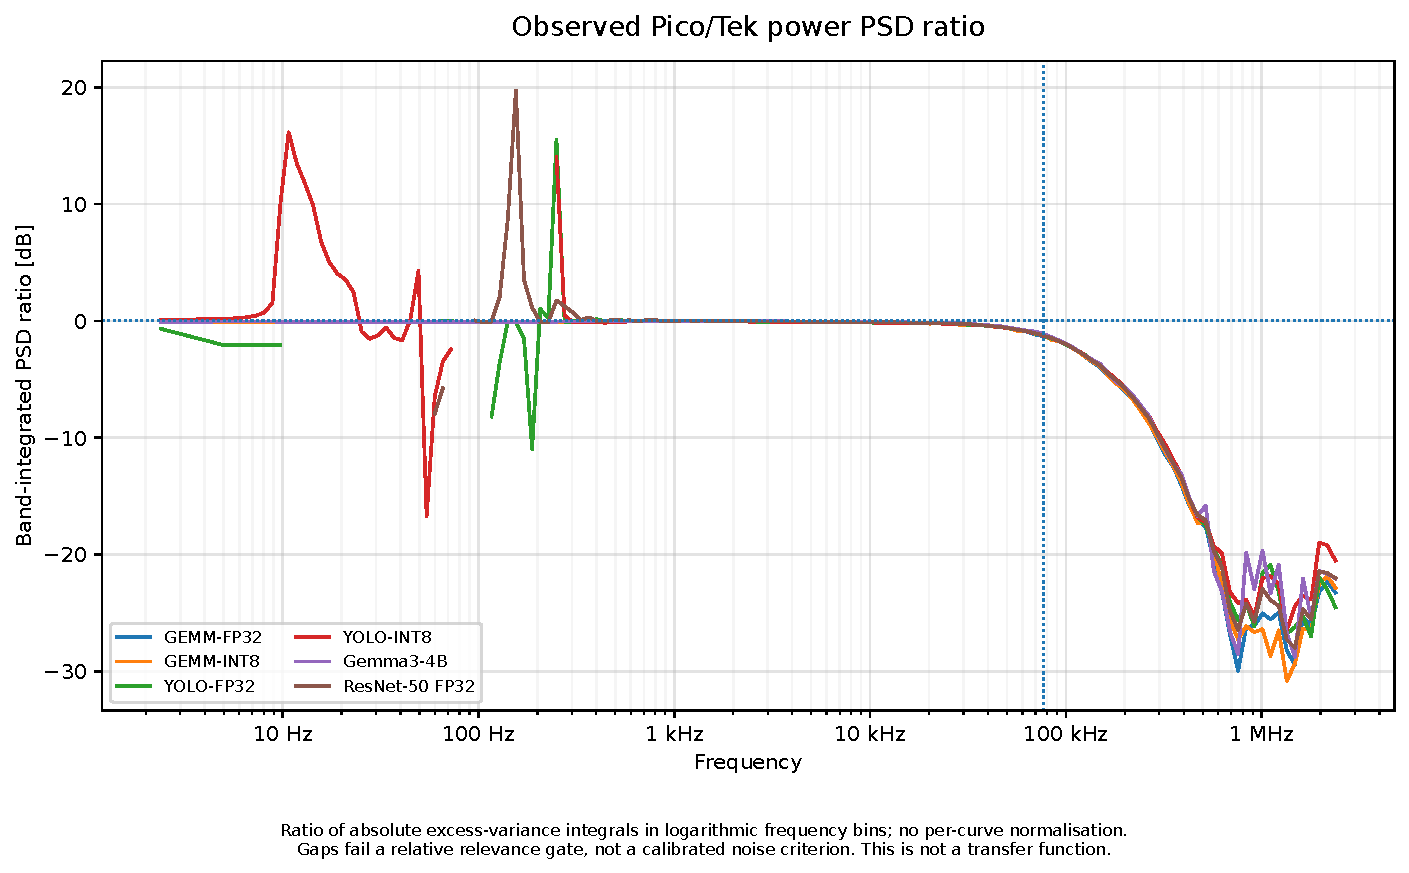
\includegraphics[width=\linewidth]{pico_vs_tek_psd/figures/tek_vs_pico_power_observed_psd_ratio.pdf}
\caption{Ratio of absolute excess-variance integrals in logarithmic frequency bins; no per-curve normalisation.
Gaps fail a relative relevance gate, not a calibrated noise criterion. This is not a transfer function.}
\label{fig:journal-pico-vs-tek-psd-figures-tek-vs-pico-power-observed-psd-ratio}
\end{figure}
